\documentclass[10pt,a4paper]{article}

\usepackage[T1]{fontenc}
\usepackage[utf8]{inputenc}
\usepackage{lmodern}
\usepackage[margin=20mm]{geometry}
\usepackage{microtype}
\usepackage{amsmath}
\usepackage{booktabs}
\usepackage{longtable}
\usepackage{pdflscape}
\usepackage{array}
\usepackage{graphicx}
\usepackage{float}
\usepackage{caption}
\usepackage{xcolor}
\usepackage{hyperref}

\hypersetup{
  colorlinks=true,
  linkcolor=blue!45!black,
  citecolor=green!35!black,
  urlcolor=blue!55!black,
  pdftitle={Measurement-Based Energy and Throughput Characterization of Embedded Radio Modules}
}
\setlength{\emergencystretch}{2em}
\setlength{\LTpre}{0.5em}
\setlength{\LTpost}{0.5em}
\renewcommand{\arraystretch}{1.08}
\newcommand{\code}[1]{\texttt{#1}}
\newcommand{\dataset}{\code{power\_profiler/comparisons}}
\newcommand{\micro}{\mu}
\newcommand{\percent}{\%}
\newcommand{\SI}[2]{\ensuremath{#1\,\mathrm{#2}}}
\newcommand{\num}[1]{#1}
% Generated by generate_study.py; do not edit by hand.
\newcommand{\BestPacketEnergyModule}{nRF24L01}
\newcommand{\BestPacketEnergy}{0.0187}
\newcommand{\LowestRxModule}{Ai-Thinker RA-01SH}
\newcommand{\LowestRxPower}{14.76}
\newcommand{\LowestTxModule}{nRF24L01}
\newcommand{\LowestTxPower}{1.695}
\newcommand{\HighestGoodputModule}{nRF24L01}
\newcommand{\HighestGoodput}{11.07}
\newcommand{\BestESeventyNineProfile}{GFSK200}
\newcommand{\BestESeventyNineEnergy}{0.108}
\newcommand{\ESeventyNineSlowEnergy}{4.150}
\newcommand{\ESeventyNineFastEnergy}{0.108}
\newcommand{\ESeventyNineImprovement}{38.5}
\newcommand{\TotalPacketRuns}{5880}
\newcommand{\TotalPacketEvaluated}{5610}
\newcommand{\TotalPacketPoints}{1176}
\newcommand{\TotalPacketReceived}{5351}
\newcommand{\TotalContinuousWindows}{270}
\newcommand{\TotalContinuousSent}{154229}
\newcommand{\TotalContinuousReceived}{124703}


\title{Measurement-Based Energy and Throughput Characterization\\
of 23 Embedded Radio Modules and Hardware Variants}
\author{Victor Stoica\\Radio Power Profiler Project}
\date{July 2026}

\begin{document}
\maketitle

\begin{abstract}
This work compares 23 embedded radio modules and physical implementations using a common measurement pipeline and a Nordic Power Profiler Kit II (PPK2). The campaign contains \TotalPacketPoints{} packet-level operating points, \TotalPacketRuns{} packet repetitions, and \TotalContinuousWindows{} 60-second traffic windows. It spans sub-GHz and \SI{2.4}{GHz} radios, direct-SPI transceivers, transparent UART modems, integrated radio microcontrollers, LoRa, 2-(G)FSK, OOK, SimpleLink Long Range, and IEEE 802.15.4g-derived profiles. Absolute TX and RX energy is reported for every logical payload size exercised by each campaign: 8, 16, 32, 58, 60, 64, 128, 512, or 1024 bytes. The common 32-byte point remains useful for a cross-module comparison, but it no longer substitutes for the measured payload curves. Matched sub-studies compare CC1101 revisions and bands, E32 bands, SX1278 board implementations, RA-02 capacitor variants, nRF24L01 PA/LNA integration, and seven CC1352P PHY profiles. Measured transmit energy spans \SI{0.0187}{mJ} to \SI{160.35}{mJ} at the common 32-byte point. Larger-payload results reveal both fixed-cost amortization and the absolute cost of fragmentation. Continuous delivery results are reported as end-to-end system behavior and are not treated as standalone RF sensitivity measurements.
\end{abstract}

\section{Introduction}

Selecting a radio for a battery-powered embedded system is not a one-dimensional choice. Nominal transmit power, data rate, receiver current, modulation, host interface, packet framing, buffering, and firmware latency all influence the energy needed to move an application payload. Datasheet currents are indispensable for design, but they do not include every module-level regulator, level shifter, external PA/LNA, transparent-UART queue, or firmware decision. Conversely, a bench measurement without a controlled workload can make two radios look comparable when their payload, airtime, or reliability differs.

This study treats the measured module as the system boundary and asks four questions:

\begin{enumerate}
  \item How widely do packet TX/RX energy and sustained-traffic power vary across the tested modules?
  \item How do logical payload size and configured rate trade against packet energy and delivered throughput?
  \item How much variation remains when the radio IC and LoRa parameters are held constant but the physical implementation changes?
  \item What changes when a single programmable radio, the E79/CC1352P, is moved among GFSK, OOK, SimpleLink Long Range (SLR), and IEEE 802.15.4g profiles?
\end{enumerate}

The contribution is an artifact-backed comparison rather than a catalog ranking. Every plotted point is generated from the consolidated CSV files in \dataset; the normalized data, plotting script, and LaTeX tables are included beside this manuscript.

\section{Devices and Tested Configuration Space}

The set includes CC1101 boards at 433 and \SI{868}{MHz}; direct-SPI and transparent-UART SX127x/SX126x/SX1280 implementations; nRF24L01 modules with and without PA/LNA; an HC-12; the E79 programmable modem; and an ASR6601-based RA-08. LoRa-capable chips frequently support additional modulations that were not exercised in their corresponding campaign. Therefore, Table~\ref{tab:catalog} lists the tested PHY, not every mode advertised by the silicon vendor. For example, the SX1276 family can also implement FSK, GFSK, MSK, GMSK, and OOK, while the SX1262 family supports LoRa, (G)FSK, and LR-FHSS \cite{semtech_sx1276,semtech_sx1262}. The SX1280 additionally supports FLRC and (G)FSK \cite{semtech_sx1280}.

{\footnotesize\setlength{\tabcolsep}{2pt}
\captionsetup{justification=raggedright,singlelinecheck=false}
\begin{longtable}{@{}>{\raggedright\arraybackslash}p{0.19\linewidth}>{\raggedright\arraybackslash}p{0.11\linewidth}>{\raggedright\arraybackslash}p{0.075\linewidth}>{\raggedright\arraybackslash}p{0.075\linewidth}>{\raggedright\arraybackslash}p{0.18\linewidth}>{\raggedright\arraybackslash}p{0.15\linewidth}>{\raggedright\arraybackslash}p{0.14\linewidth}@{}}
\caption{Measured module and hardware-variant catalog. Rates and powers are the settings exercised in this campaign, not the full capabilities of each chipset.}\label{tab:catalog}\\
\toprule
Module/variant & Radio IC & Band & I/F & Tested PHY/modulation & Tested rates & Tested power \\ \midrule
\endfirsthead
\toprule Module/variant & Radio IC & Band & I/F & Tested PHY/modulation & Tested rates & Tested power \\ \midrule
\endhead
CC1101 V1 433 MHz & CC1101 & 433 MHz & SPI & 2-FSK & 1.2/38.4/250 kbps & -30/0/10 dBm \\
CC1101 V2 868 MHz & CC1101 & 868 MHz & SPI & 2-FSK & 1.2/38.4/250 kbps & -30/0/10 dBm \\
E28 direct SPI & SX1280 & 2.4 GHz & SPI & LoRa, CR 4/6 & SF5/8/12, BW 812.5 kHz & -18/0/13 dBm \\
Ebyte E280-2G4T12S & SX1280 & 2.4 GHz & UART & Vendor transparent PHY & 1/100/2000 kbps presets & 4/7/12 dBm \\
Ebyte E22-400M30S & SX1268 + PA & 433 MHz & SPI & LoRa, CR 4/5 & SF7/9/12, BW 125 kHz & -9/10/18 dBm front stage \\
Ebyte E32-433T20D & SX1278 & 433 MHz & UART & LoRa transparent, FEC & 0.3/4.8/19.2 kbps & 10/14/20 dBm \\
Ebyte E32-433T33D & SX1278 + PA & 433 MHz & UART & LoRa transparent, FEC & 0.3/4.8/19.2 kbps & 24/27/30 dBm \\
Ebyte E32-868T20D & SX1276 & 868 MHz & UART & LoRa transparent, FEC & 0.3/4.8/19.2 kbps & 10/14/20 dBm \\
Ebyte E32-868T30D & SX1276 + PA & 868 MHz & UART & LoRa transparent, FEC & 0.3/4.8/19.2 kbps & 21/27/30 dBm \\
Ebyte E79-400DM2005S & CC1352P & 433 MHz & UART AT & 2-GFSK, OOK, SLR, 802.15.4g & 2.5--200 kbps (7 PHYs) & -20/0/13 dBm \\
HC-12 & Si4463 & 433 MHz & UART & Transparent (G)FSK & 0.5/15/250 kbps presets & -1/8/20 dBm \\
nRF24L01 & nRF24L01+ & 2.4 GHz & SPI & GFSK, ESB framing & 250/1000/2000 kbps & -18/-6/0 dBm \\
nRF24L01+PA/LNA & nRF24L01+ + PA/LNA & 2.4 GHz & SPI & GFSK, ESB framing & 250/1000/2000 kbps & -18/-6/0 dBm drive \\
Ai-Thinker RA-01H & SX1276 & 868 MHz & SPI & LoRa, CR 4/5 & SF7/9/12, BW 125 kHz & 2/10/20 dBm \\
Ai-Thinker RA-01SH & SX1262 & 868 MHz & SPI & LoRa, CR 4/5 & SF7/9/12, BW 125 kHz & -9/10/22 dBm \\
Ai-Thinker RA-02 & SX1278 & 433 MHz & SPI & LoRa, CR 4/5 & SF7/9/12, BW 125 kHz & -4/10/20 dBm \\
Ai-Thinker RA-02 + 2 capacitors & SX1278 & 433 MHz & SPI & LoRa, CR 4/5 & SF7/9/12, BW 125 kHz & -4/10/20 dBm \\
Ai-Thinker RA-08 & ASR6601 & 433 MHz & UART AT & LoRa, CR 4/5 & SF7/9/12, BW 125 kHz & 2/12/22 dBm \\
SX1278 + level shifter & SX1278 & 433 MHz & SPI & LoRa, CR 4/5 & SF7/9/12, BW 125 kHz & -4/10/20 dBm \\
SX1278 naked board & SX1278 & 433 MHz & SPI & LoRa, CR 4/5 & SF7/9/12, BW 125 kHz & -4/10/20 dBm \\
SX1278 PCB + 2 capacitors & SX1278 & 433 MHz & SPI & LoRa, CR 4/5 & SF7/9/12, BW 125 kHz & -4/10/20 dBm \\
SX1278 shielded board & SX1278 & 433 MHz & SPI & LoRa, CR 4/5 & SF7/9/12, BW 125 kHz & -4/10/20 dBm \\
XL1276-D01 & SX1276 & 433 MHz & SPI & LoRa, CR 4/5 & SF7/9/12, BW 125 kHz & -4/10/20 dBm \\
\bottomrule
\end{longtable}

}

The E79 campaign is intentionally broader than the others. Its CC1352P supports programmable proprietary formats and multiple modulation families \cite{ti_cc1352p}; the measured firmware exposes seven fixed profiles from \SI{2.5}{kbps} through \SI{200}{kbps}. The E32 devices, in contrast, expose vendor air-rate presets through a transparent UART interface. Their nominal setting is useful for configuration and pacing, but it is not equivalent to application goodput.

\section{Measurement Method}

\subsection{Instrumentation and boundary}

Current was measured with a Nordic PPK2 in ampere-meter mode at a recorded DUT supply of \SI{3.3}{V} and a sampling rate of \SI{100}{kSa.s^{-1}}. The PPK2 supports \SI{100}{kSa.s^{-1}} acquisition and automatically switches current ranges; its documented average-current accuracy is better than $\pm 20\%$ \cite{nordic_ppk2}. The latter is an instrument-level bound, not the uncertainty of the sample mean, and should be retained when using small differences for design decisions.

The measured boundary is the powered radio module or radio board under test. Consequently, a result may include the radio IC, module regulator, TCXO, level shifter, onboard MCU, or external PA/LNA, depending on the implementation. USB bridges and the host PC are outside that power boundary. This is deliberate: the goal is deployable module energy, not transistor-level RF-core current.

\subsection{Packet campaign}

Each packet operating point was repeated five times. Payload matrices were module-appropriate, but all devices include a 32-byte payload. Across the complete dataset, the measured logical payload sizes are 8, 16, 32, 58, 60, 64, 128, 512, and 1024 bytes. The 58-byte E32 and 60-byte HC-12 points reflect campaign-validated frame boundaries; they must not be silently treated as 64-byte observations. The campaign records total event energy, event duration, mean and peak current, sample loss, configuration, status, and packet-delivery telemetry. Larger logical payloads are fragmented when a module has a smaller physical FIFO or validated frame size. Total event energy is used here because it captures startup, framing, transparent-modem latency, and the active receive window. Baseline-subtracted metrics remain available in the source artifacts for analyses focused specifically on incremental RF activity.

For a current trace $I(t)$ at supply voltage $V$, total event energy is
\begin{equation}
  E_{\mathrm{event}} = V \int_{t_0}^{t_1} I(t)\,\mathrm{d}t.
\end{equation}
For secondary normalization, the useful-bit metric for payload length $L$ bytes is
\begin{equation}
  e_b = \frac{E_{\mathrm{event}}}{8L}.
\end{equation}
It is retained in the generated CSV for derived analysis, but it is not the principal table metric. A single $e_b$ value can obscure the actual energy of a message and any fragmentation boundary. Therefore, the manuscript reports measured $E_{\mathrm{event}}$ in millijoules at each tested payload size. Preamble, sync, headers, coding, CRC, command latency, and fragmentation are intentionally not counted as useful bits in the secondary metric.

\subsection{Continuous traffic campaign}

Continuous tests use \SI{60}{s} windows with repeated frames and a campaign-defined host gap. Average current and power are computed over the active window,
\begin{equation}
  \bar{I}=\frac{1}{T}\int_0^T I(t)\,\mathrm{d}t,
  \qquad \bar{P}=V\bar{I}.
\end{equation}
The comparative power-versus-RF-setting figures also report the increment above the \SI{100}{ms} pre-trigger standby baseline,
\begin{equation}
  \bar{P}_{\mathrm{excess}}=V\max\!\left(0,\bar{I}-\bar{I}_{\mathrm{standby}}\right).
\end{equation}
The clamp is part of the acquisition pipeline. Consequently, a zero excess-power point means that the active-window mean did not exceed that session's baseline; it does not mean that the radio consumed zero power. The total-power panel remains the battery-budget quantity.
Received useful goodput is
\begin{equation}
  G_{RX}=\frac{8L_cN_{RX}}{T},
\end{equation}
where $L_c$ is the useful content per repeated frame and $N_{RX}$ is the number of frames reported by the receiver. The delivery ratio is $100N_{RX}/N_{TX}$.

These windows are sustained host-driven traffic, not necessarily a radio held continuously in the TX state. Average TX power can therefore be low for short packets separated by the host gap. Likewise, lost frames can result from receiver re-arm latency, UART buffering, serial parsing, or power integrity in addition to RF propagation.

\subsection{Normalization and audit rules}

For every measured payload size, the packet matrix selects the fastest tested packet mode and highest tested configured power for that module. TX and RX rows are required to use the same mode and power. The common cross-module point is the 32-byte column under the same rule. This compares useful design operating points but not equal range, sensitivity, EIRP, occupied bandwidth, or regulatory duty cycle. A dash in a payload table means \emph{not measured}, never zero energy or an interpolated estimate. LoRa gross rate is estimated as
\begin{equation}
  R_b = \frac{BW}{2^{SF}}\,SF\,\frac{4}{CR_d},
\end{equation}
with $CR_d=5$ for CR~4/5 and $CR_d=6$ for the E28 CR~4/6 campaign. Transparent-modem and FSK points use their configured rate labels.

For continuous power, the fastest mode actually present among TX windows is selected and the RX row is matched to the same mode and power. This is often the campaign's representative middle mode (for example SF9), not the fastest packet mode. Aggregate packet and continuous delivery ratios retain the full configuration matrix.

Modern consolidated files contain explicit attempted and received counters. Older files use the number of runs as the denominator. CC1101 V2 has receiver-side delivery telemetry but no TX-measurement peer telemetry; its packet delivery value is therefore computed from the 90 receiver-side repetitions and is marked \emph{RX-only legacy telemetry}. Missing TX telemetry is not counted as RF loss. Of \TotalPacketRuns{} measured packet repetitions, \TotalPacketEvaluated{} have usable delivery telemetry under these rules.

\section{Results}

\subsection{Cross-module benchmark}

Tables~\ref{tab:packet-tx-matrix} and~\ref{tab:packet-rx-matrix} report the measured mean energy of one logical packet for every payload size available in each module campaign. Each populated cell is backed by five packet repetitions at the stated mode and power. The tables deliberately retain different payload limits instead of extrapolating modules beyond the tested workload.

\clearpage
\begin{landscape}
{\footnotesize\setlength{\tabcolsep}{6pt}
\begin{table}[p]
\centering
\caption{Measured TX energy per logical packet at each module's fastest tested mode and highest tested configured power. Payload columns are bytes; a dash means that payload size was not measured.}
\label{tab:packet-tx-matrix}
\resizebox{\textwidth}{!}{%
\begin{tabular}{@{}llrrrrrrrrrr@{}}
\toprule
ID & Mode & dBm & 8 & 16 & 32 & 58 & 60 & 64 & 128 & 512 & 1024 \\
 & & & [mJ] & [mJ] & [mJ] & [mJ] & [mJ] & [mJ] & [mJ] & [mJ] & [mJ] \\ \midrule
C11-433 & 250 kbps & 10.00 & 0.19 & \textemdash & 0.32 & \textemdash & \textemdash & 0.729 & 1.536 & 6.390 & 12.87 \\
C11-868 & 250 kbps & 10.00 & 0.122 & \textemdash & 0.201 & \textemdash & \textemdash & 0.478 & 1.037 & 4.397 & 8.874 \\
E28 & SF5 & 13.00 & 0.212 & \textemdash & 0.417 & \textemdash & \textemdash & \textemdash & 1.306 & \textemdash & \textemdash \\
E280 & 2000 kbps & 12.00 & 0.0249 & \textemdash & 0.0362 & \textemdash & \textemdash & 0.0507 & \textemdash & \textemdash & \textemdash \\
E22 & SF7 & 18.00 & 9.252 & \textemdash & 17.74 & \textemdash & \textemdash & \textemdash & 51.66 & \textemdash & \textemdash \\
E32-43-20 & 19.2 kbps & 20.00 & 7.911 & \textemdash & 17.69 & 28.47 & \textemdash & \textemdash & 66.32 & 249.8 & 498.8 \\
E32-43-33 & 19.2 kbps & 30.00 & 78.92 & \textemdash & 160.4 & 241.3 & \textemdash & \textemdash & 516.0 & 1902.1 & 3820.3 \\
E32-86-20 & 19.2 kbps & 20.00 & 7.910 & \textemdash & 17.66 & 28.36 & \textemdash & \textemdash & 66.05 & 248.9 & 498.1 \\
E32-86-30 & 19.2 kbps & 30.00 & 41.75 & \textemdash & 91.65 & 146.9 & \textemdash & \textemdash & 343.4 & 1298.4 & 2590.6 \\
E79 & GFSK200 & 13.00 & 0.0757 & \textemdash & 0.108 & \textemdash & \textemdash & 0.152 & 0.246 & 0.857 & 1.660 \\
HC-12 & 250 kbps & 20.00 & 3.562 & \textemdash & 5.413 & \textemdash & 9.186 & \textemdash & \textemdash & \textemdash & \textemdash \\
NRF & 2000 kbps & 0 & 0.0125 & 0.015 & 0.0187 & \textemdash & \textemdash & \textemdash & \textemdash & \textemdash & \textemdash \\
NRF-PA & 2000 kbps & 0 & 0.0496 & 0.0659 & 0.0935 & \textemdash & \textemdash & \textemdash & \textemdash & \textemdash & \textemdash \\
RA-01H & SF7 & 20.00 & 16.57 & \textemdash & 30.24 & \textemdash & \textemdash & \textemdash & 85.00 & \textemdash & \textemdash \\
RA-01SH & SF7 & 22.00 & 9.897 & \textemdash & 18.03 & \textemdash & \textemdash & \textemdash & 50.60 & \textemdash & \textemdash \\
RA-02 & SF7 & 20.00 & 9.143 & \textemdash & 16.67 & \textemdash & \textemdash & \textemdash & 46.67 & \textemdash & \textemdash \\
RA-02-2C & SF7 & 20.00 & 8.845 & \textemdash & 16.17 & \textemdash & \textemdash & \textemdash & 45.40 & \textemdash & \textemdash \\
RA-08 & SF7 & 22.00 & 16.51 & \textemdash & 32.84 & \textemdash & \textemdash & \textemdash & 98.05 & \textemdash & \textemdash \\
S1278-LS & SF7 & 20.00 & 12.08 & \textemdash & 23.27 & \textemdash & \textemdash & \textemdash & 68.09 & \textemdash & \textemdash \\
S1278-N & SF7 & 20.00 & 10.61 & \textemdash & 19.36 & \textemdash & \textemdash & \textemdash & 54.40 & \textemdash & \textemdash \\
S1278-2C & SF7 & 20.00 & 10.51 & \textemdash & 19.20 & \textemdash & \textemdash & \textemdash & 54.06 & \textemdash & \textemdash \\
S1278-S & SF7 & 20.00 & 11.57 & \textemdash & 22.32 & \textemdash & \textemdash & \textemdash & 65.11 & \textemdash & \textemdash \\
XL1276 & SF7 & 20.00 & 10.71 & \textemdash & 21.35 & \textemdash & \textemdash & \textemdash & 63.61 & \textemdash & \textemdash \\
\bottomrule
\end{tabular}%
}
\end{table}

}
\end{landscape}

\clearpage
\begin{landscape}
{\footnotesize\setlength{\tabcolsep}{6pt}
\begin{table}[p]
\centering
\caption{Measured RX energy per logical packet at each module's fastest tested mode and highest tested configured power. Payload columns are bytes; a dash means that payload size was not measured.}
\label{tab:packet-rx-matrix}
\resizebox{\textwidth}{!}{%
\begin{tabular}{@{}llrrrrrrrrrr@{}}
\toprule
ID & Mode & dBm & 8 & 16 & 32 & 58 & 60 & 64 & 128 & 512 & 1024 \\
 & & & [mJ] & [mJ] & [mJ] & [mJ] & [mJ] & [mJ] & [mJ] & [mJ] & [mJ] \\ \midrule
C11-433 & 250 kbps & 10.00 & 5.898 & \textemdash & 6.177 & \textemdash & \textemdash & 6.942 & 8.648 & 18.78 & 32.21 \\
C11-868 & 250 kbps & 10.00 & 5.731 & \textemdash & 5.990 & \textemdash & \textemdash & 6.781 & 8.394 & 18.31 & 31.69 \\
E28 & SF5 & 13.00 & 0.0466 & \textemdash & 0.0998 & \textemdash & \textemdash & \textemdash & 0.295 & \textemdash & \textemdash \\
E280 & 2000 kbps & 12.00 & 0.589 & \textemdash & 0.594 & \textemdash & \textemdash & 0.602 & \textemdash & \textemdash & \textemdash \\
E22 & SF7 & 18.00 & 0.672 & \textemdash & 1.327 & \textemdash & \textemdash & \textemdash & 3.978 & \textemdash & \textemdash \\
E32-43-20 & 19.2 kbps & 20.00 & 1.926 & \textemdash & 3.081 & 4.327 & \textemdash & \textemdash & 10.80 & 38.65 & 77.06 \\
E32-43-33 & 19.2 kbps & 30.00 & 5.644 & \textemdash & 10.37 & 15.57 & \textemdash & \textemdash & 37.48 & 136.5 & 274.4 \\
E32-86-20 & 19.2 kbps & 20.00 & 1.923 & \textemdash & 3.081 & 4.328 & \textemdash & \textemdash & 10.82 & 38.64 & 77.14 \\
E32-86-30 & 19.2 kbps & 30.00 & 2.995 & \textemdash & 4.884 & 6.921 & \textemdash & \textemdash & 19.46 & 70.34 & 141.6 \\
E79 & GFSK200 & 13.00 & 0.0895 & \textemdash & 0.112 & \textemdash & \textemdash & 0.142 & 0.285 & 1.136 & 2.276 \\
HC-12 & 250 kbps & 20.00 & 0.337 & \textemdash & 0.358 & \textemdash & 0.398 & \textemdash & \textemdash & \textemdash & \textemdash \\
NRF & 2000 kbps & 0 & 0.0524 & 0.0539 & 0.0567 & \textemdash & \textemdash & \textemdash & \textemdash & \textemdash & \textemdash \\
NRF-PA & 2000 kbps & 0 & 0.0864 & 0.0884 & 0.0937 & \textemdash & \textemdash & \textemdash & \textemdash & \textemdash & \textemdash \\
RA-01H & SF7 & 20.00 & 1.562 & \textemdash & 2.860 & \textemdash & \textemdash & \textemdash & 8.042 & \textemdash & \textemdash \\
RA-01SH & SF7 & 22.00 & 0.654 & \textemdash & 1.185 & \textemdash & \textemdash & \textemdash & 3.316 & \textemdash & \textemdash \\
RA-02 & SF7 & 20.00 & 1.757 & \textemdash & 3.238 & \textemdash & \textemdash & \textemdash & 9.157 & \textemdash & \textemdash \\
RA-02-2C & SF7 & 20.00 & 1.761 & \textemdash & 3.245 & \textemdash & \textemdash & \textemdash & 9.183 & \textemdash & \textemdash \\
RA-08 & SF7 & 22.00 & 1.554 & \textemdash & 3.087 & \textemdash & \textemdash & \textemdash & 9.219 & \textemdash & \textemdash \\
S1278-LS & SF7 & 20.00 & 1.454 & \textemdash & 2.917 & \textemdash & \textemdash & \textemdash & 8.777 & \textemdash & \textemdash \\
S1278-N & SF7 & 20.00 & 1.366 & \textemdash & 2.729 & \textemdash & \textemdash & \textemdash & 8.169 & \textemdash & \textemdash \\
S1278-2C & SF7 & 20.00 & 1.398 & \textemdash & 2.790 & \textemdash & \textemdash & \textemdash & 8.354 & \textemdash & \textemdash \\
S1278-S & SF7 & 20.00 & 1.478 & \textemdash & 2.972 & \textemdash & \textemdash & \textemdash & 8.936 & \textemdash & \textemdash \\
XL1276 & SF7 & 20.00 & 1.459 & \textemdash & 2.934 & \textemdash & \textemdash & \textemdash & 8.826 & \textemdash & \textemdash \\
\bottomrule
\end{tabular}%
}
\end{table}

}
\end{landscape}
\clearpage

At the common 32-byte point, TX energy spans more than four orders of magnitude: \SI{0.0187}{mJ} for the nRF24L01 at \SI{2}{Mbps} and \SI{0}{dBm}, versus \SI{160.35}{mJ} for the E32-433T33D at its \SI{19.2}{kbps}, \SI{30}{dBm} setting. This is not a same-link-budget comparison. It quantifies the cost of each module's fastest measured, maximum-power operating point for an actual 32-byte application message.

\begin{figure}[htbp]
  \centering
  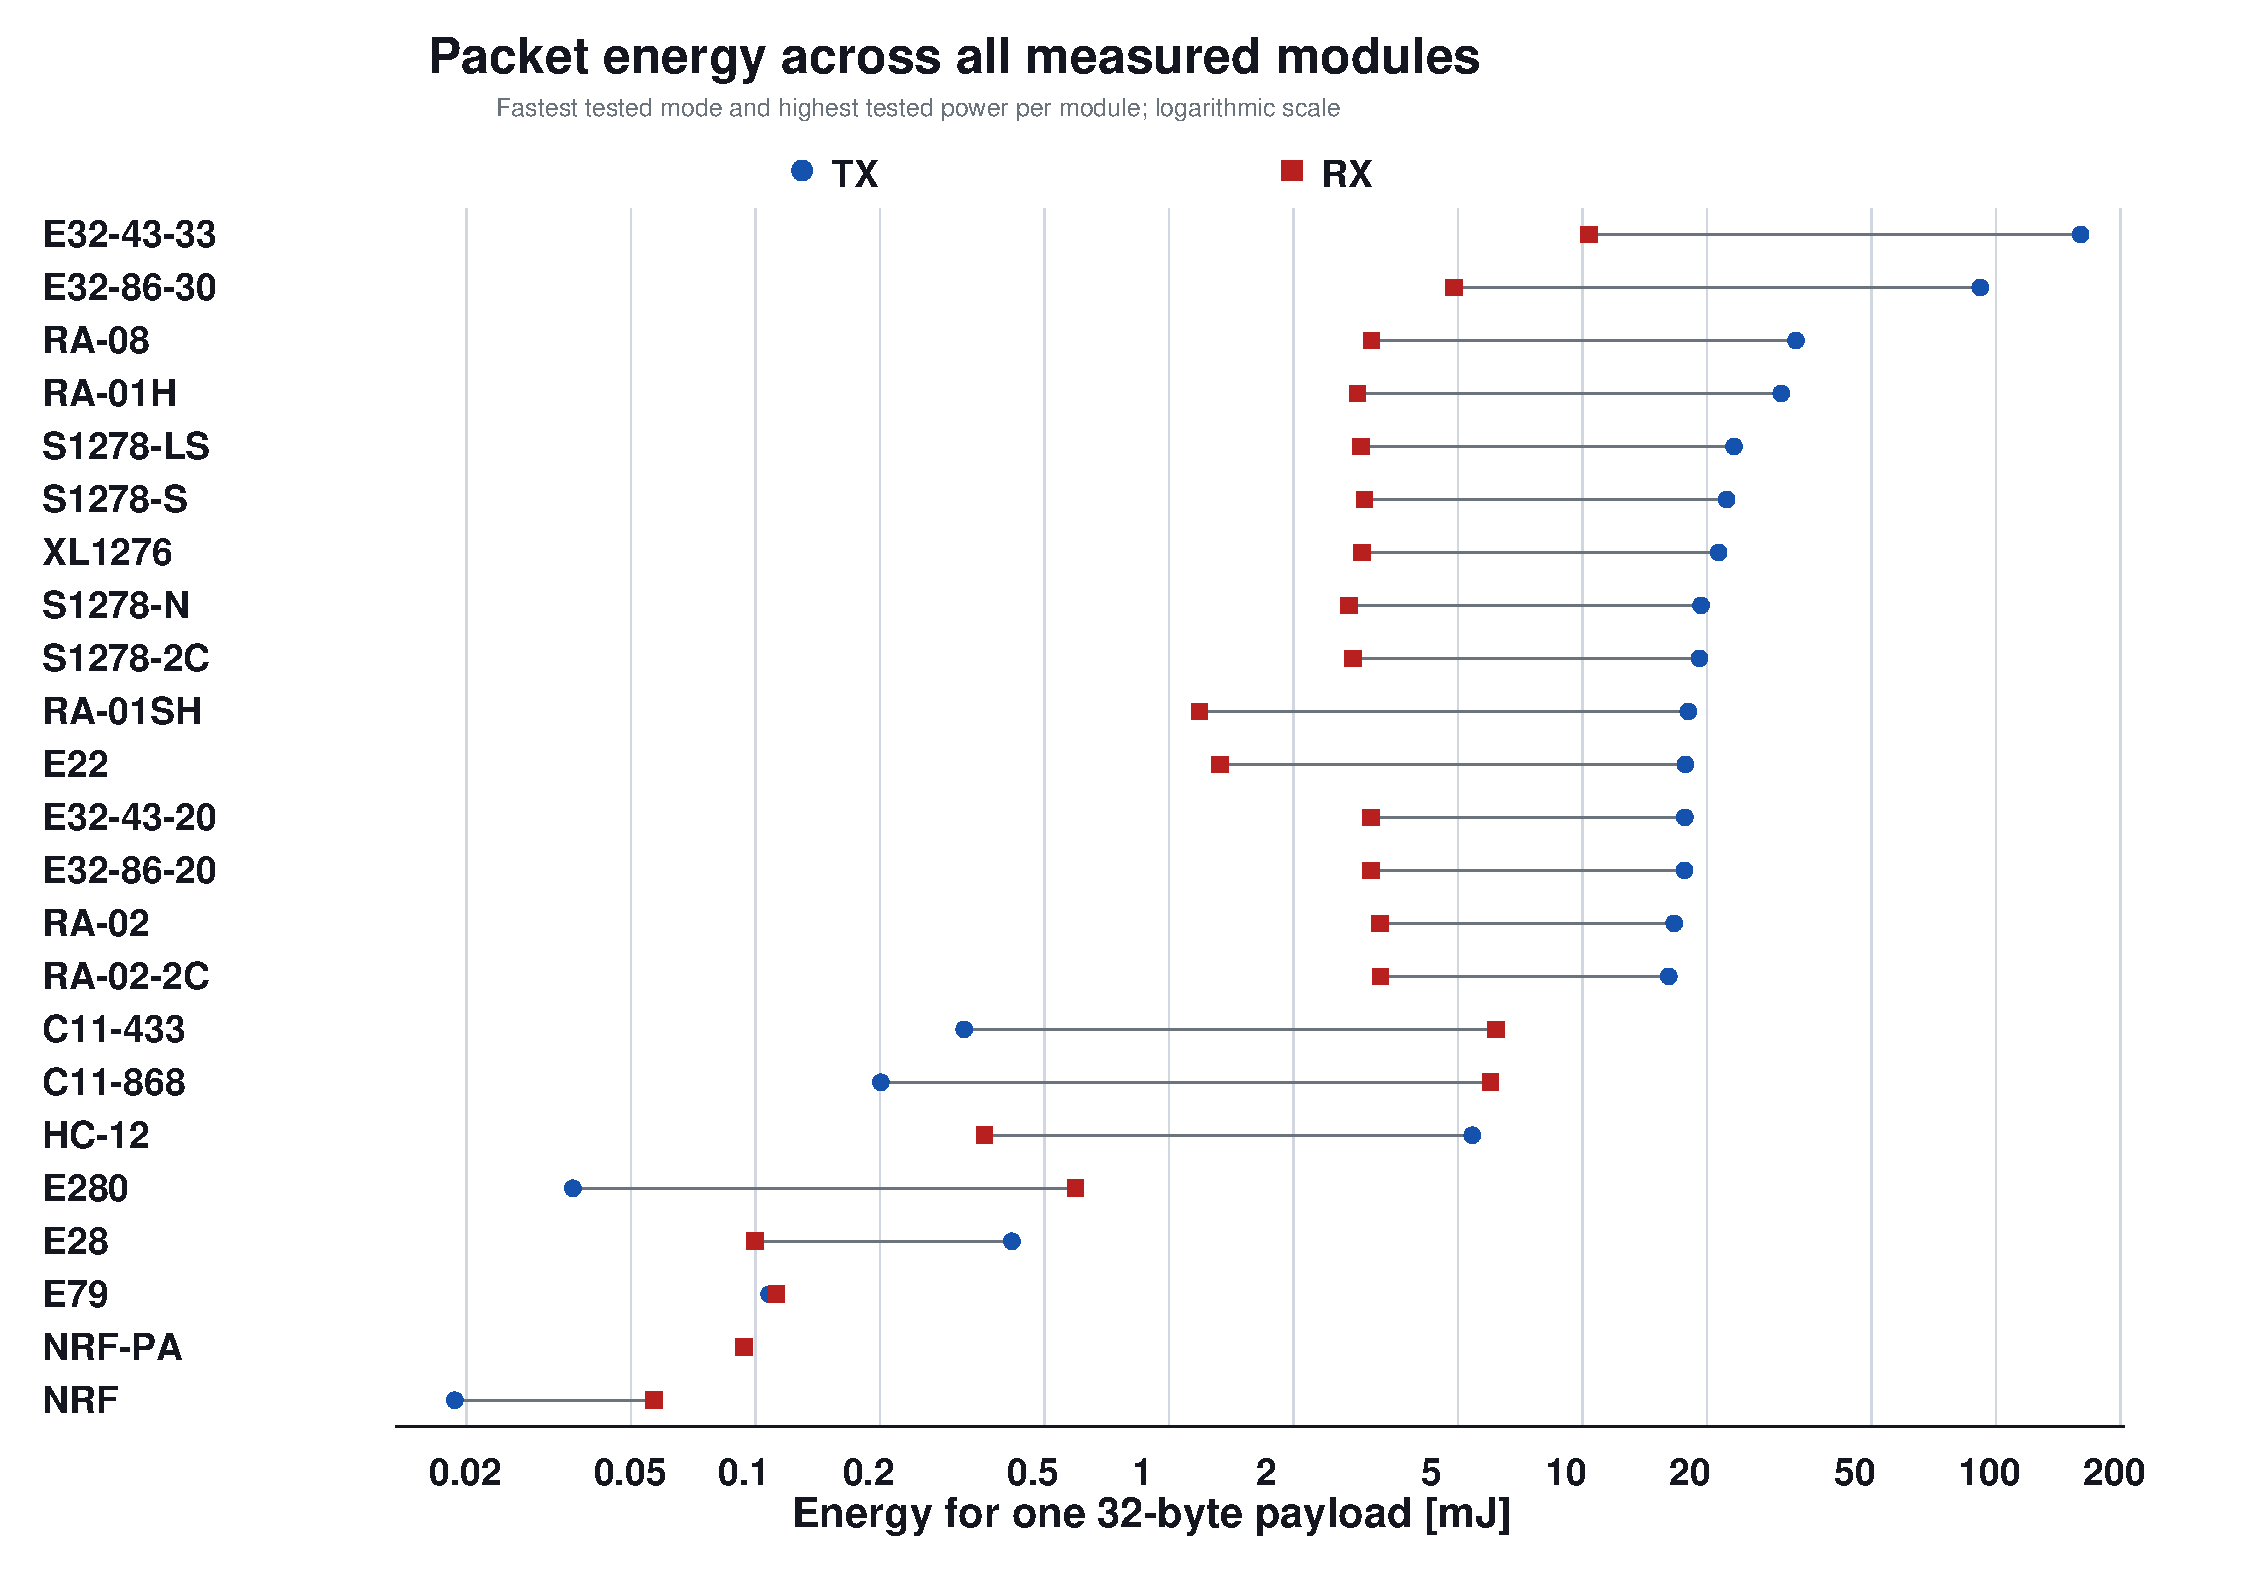
\includegraphics[width=\linewidth]{figures/packet_energy_comparison.pdf}
  \caption{Total TX and RX event energy for a common 32-byte application payload. Logarithmic scaling is necessary because both air rate and output stage vary widely.}
  \label{fig:packet-energy}
\end{figure}

TX and RX are not symmetric. Fast direct radios such as nRF24L01, E28, and E79 have sub-millijoule packet points, while receive integration windows make CC1101 RX energy much larger than its TX event at the fastest rate. The transparent E32 modules show the opposite pattern at high output power: their long, high-current TX path dominates. These differences caution against estimating bidirectional node lifetime from a TX-current headline alone.

\subsection{Payload scaling and fragmentation}

\begin{figure}[p]
  \centering
  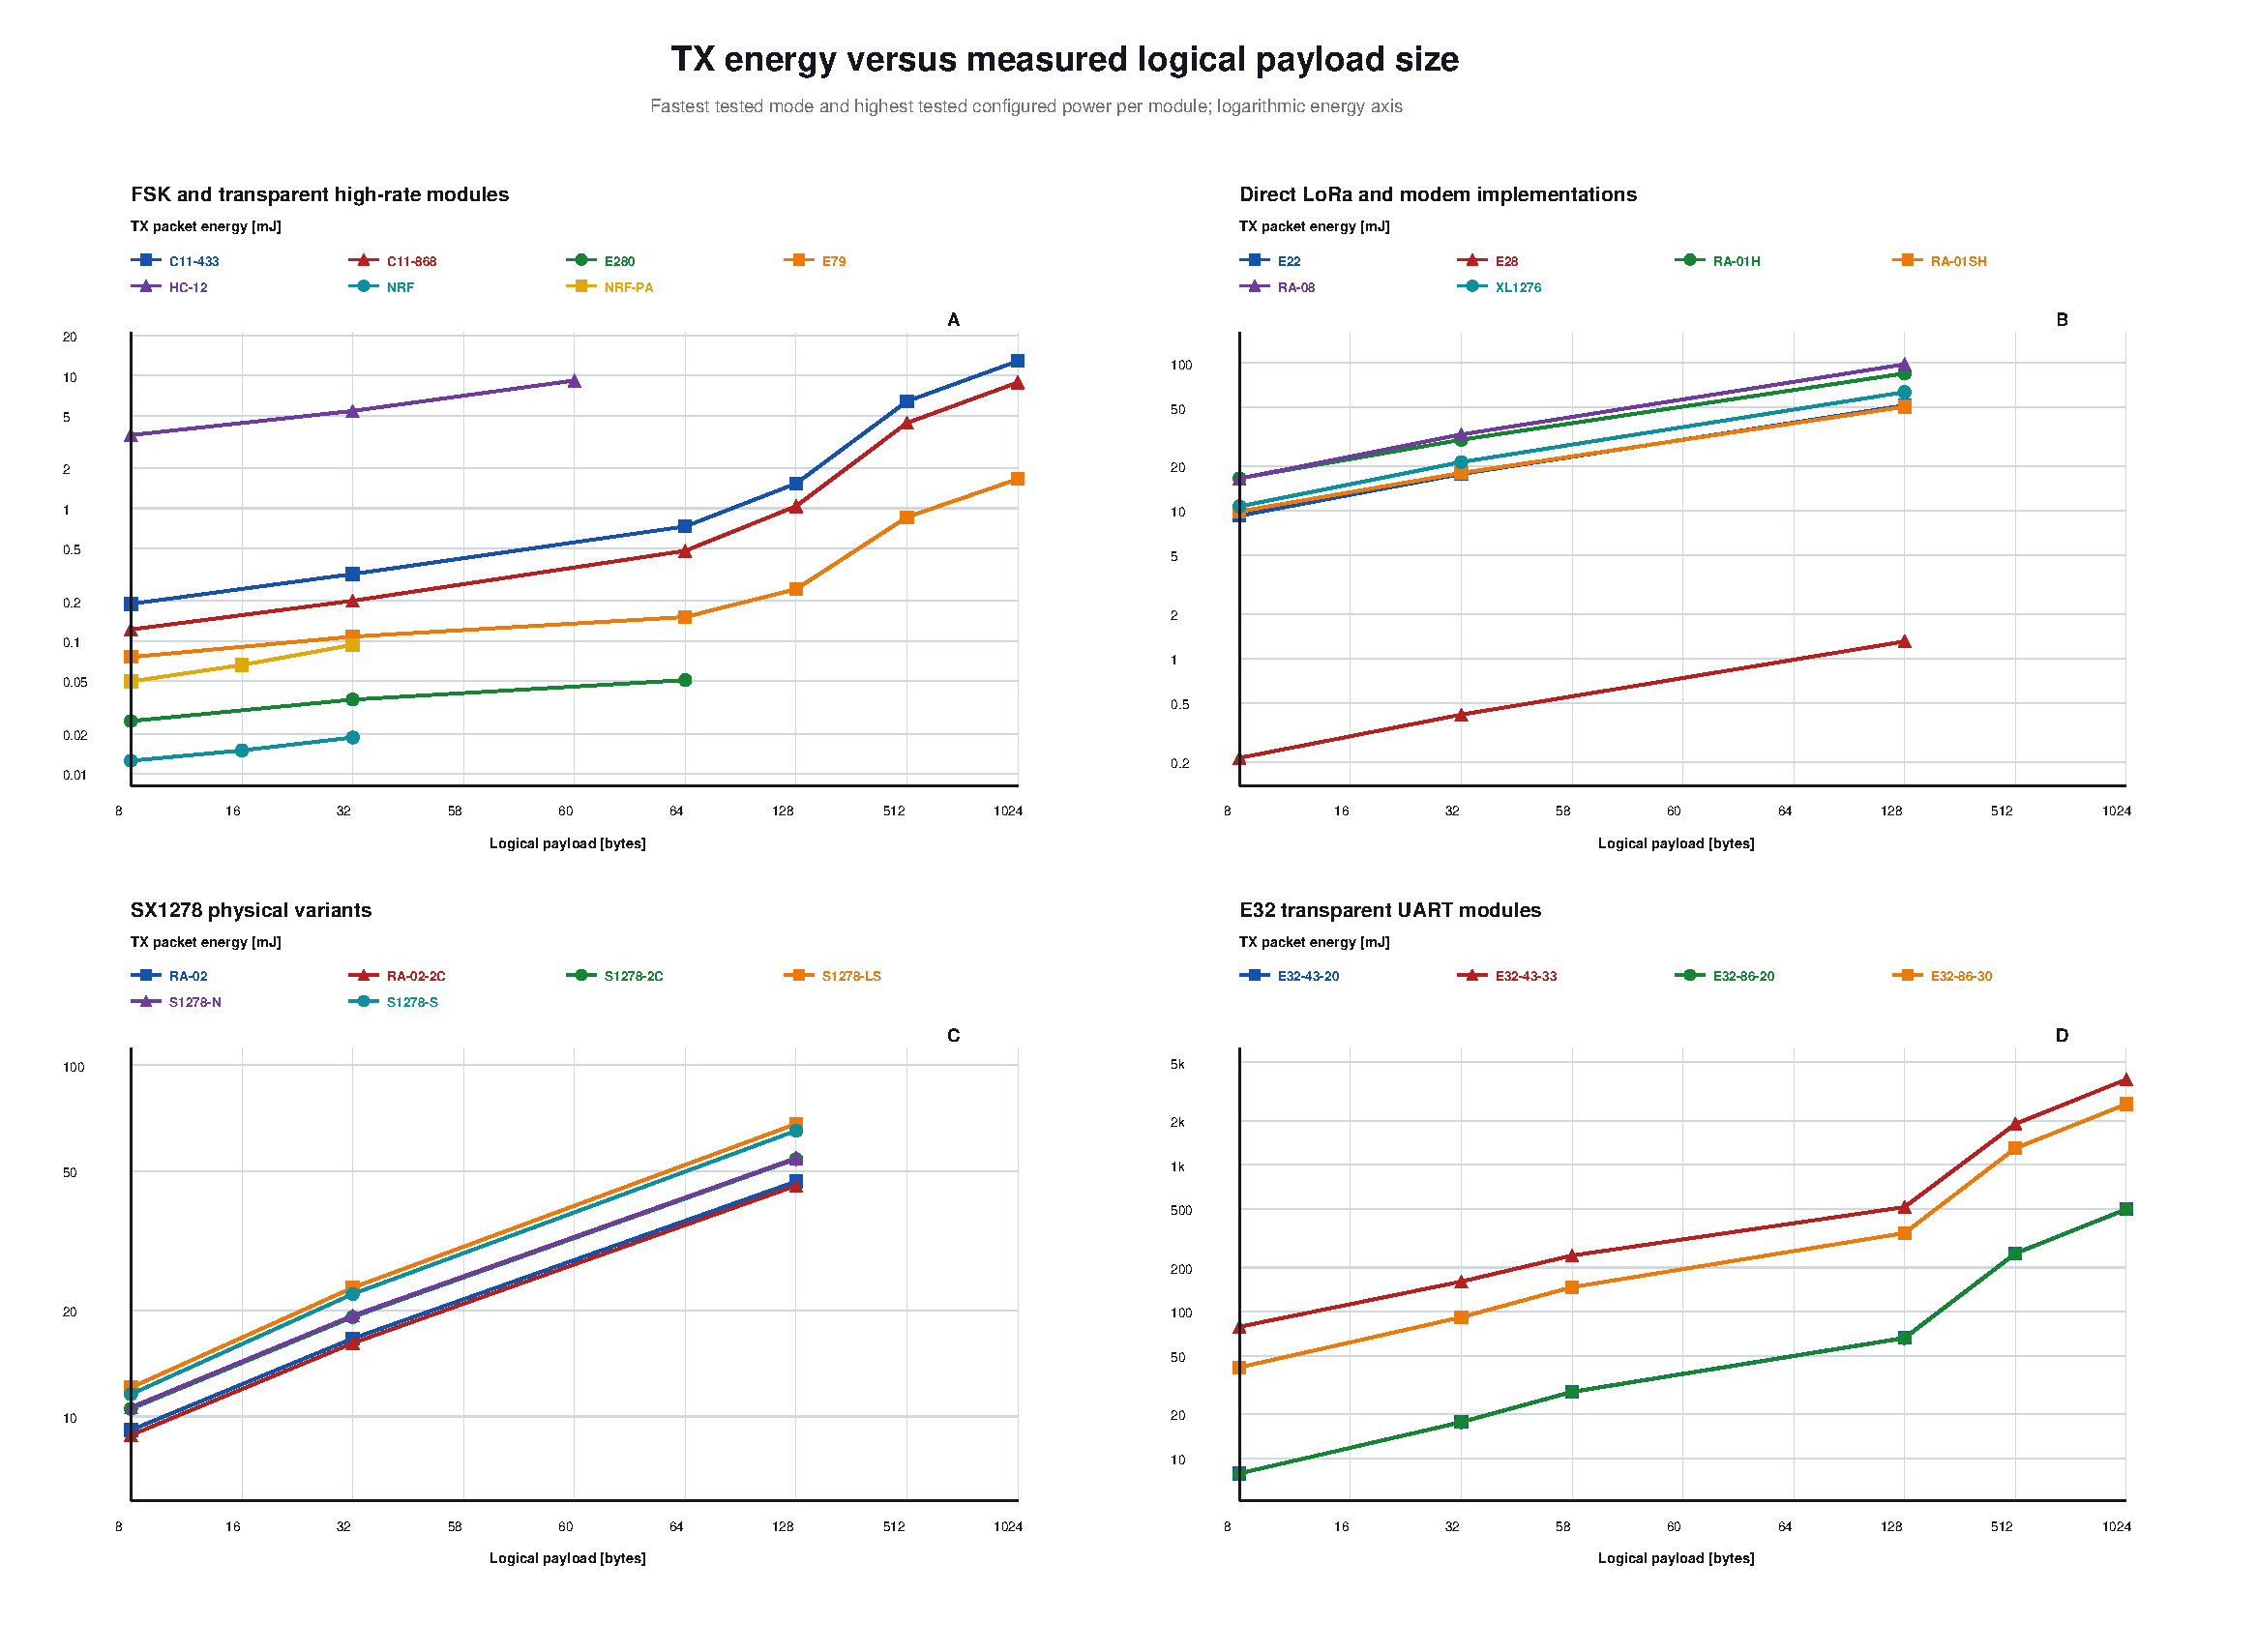
\includegraphics[width=\linewidth]{figures/tx_energy_by_payload.pdf}
  \caption{Measured TX event energy versus logical payload size, panels A--B. Lines connect measured points only; absent sizes are not interpolated in the numerical tables. Energy uses a logarithmic axis independently in each panel.}
  \label{fig:tx-payload}
\end{figure}

\begin{figure}[p]
  \centering
  \ContinuedFloat
  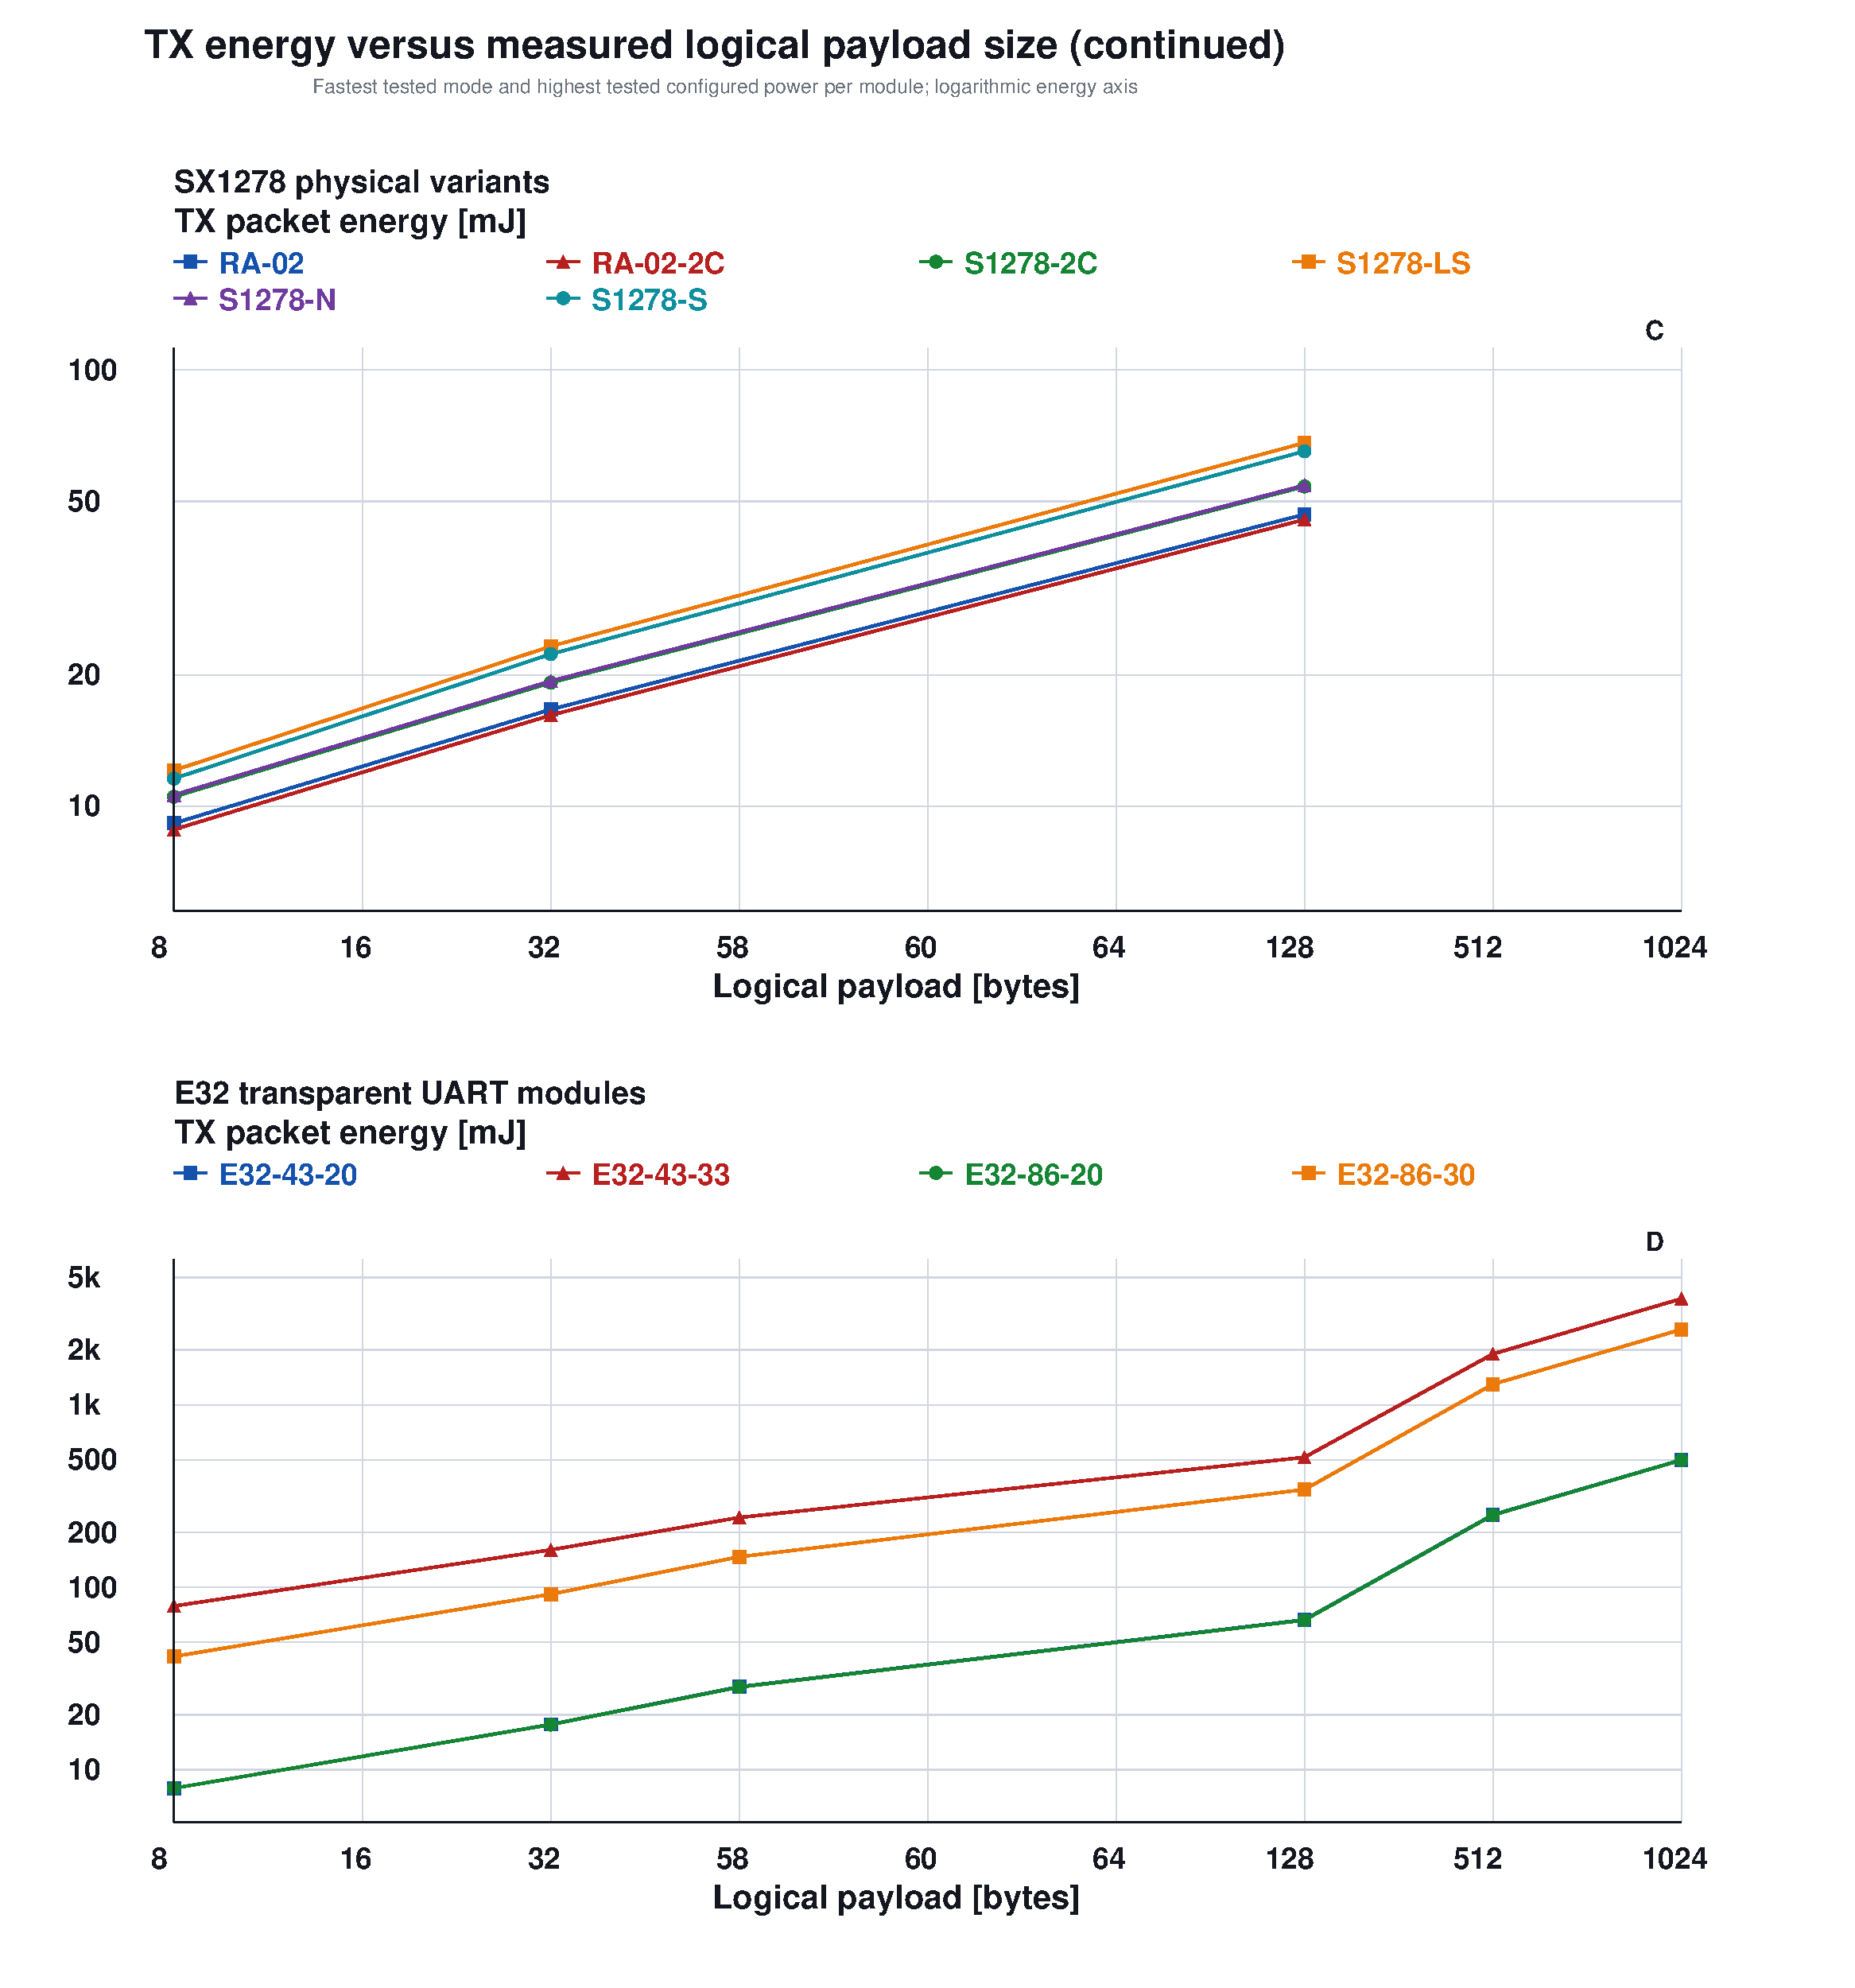
\includegraphics[width=\linewidth]{figures/tx_energy_by_payload_continued.pdf}
  \caption{Measured TX event energy versus logical payload size, panels C--D (continued).}
\end{figure}
\clearpage

\begin{figure}[p]
  \centering
  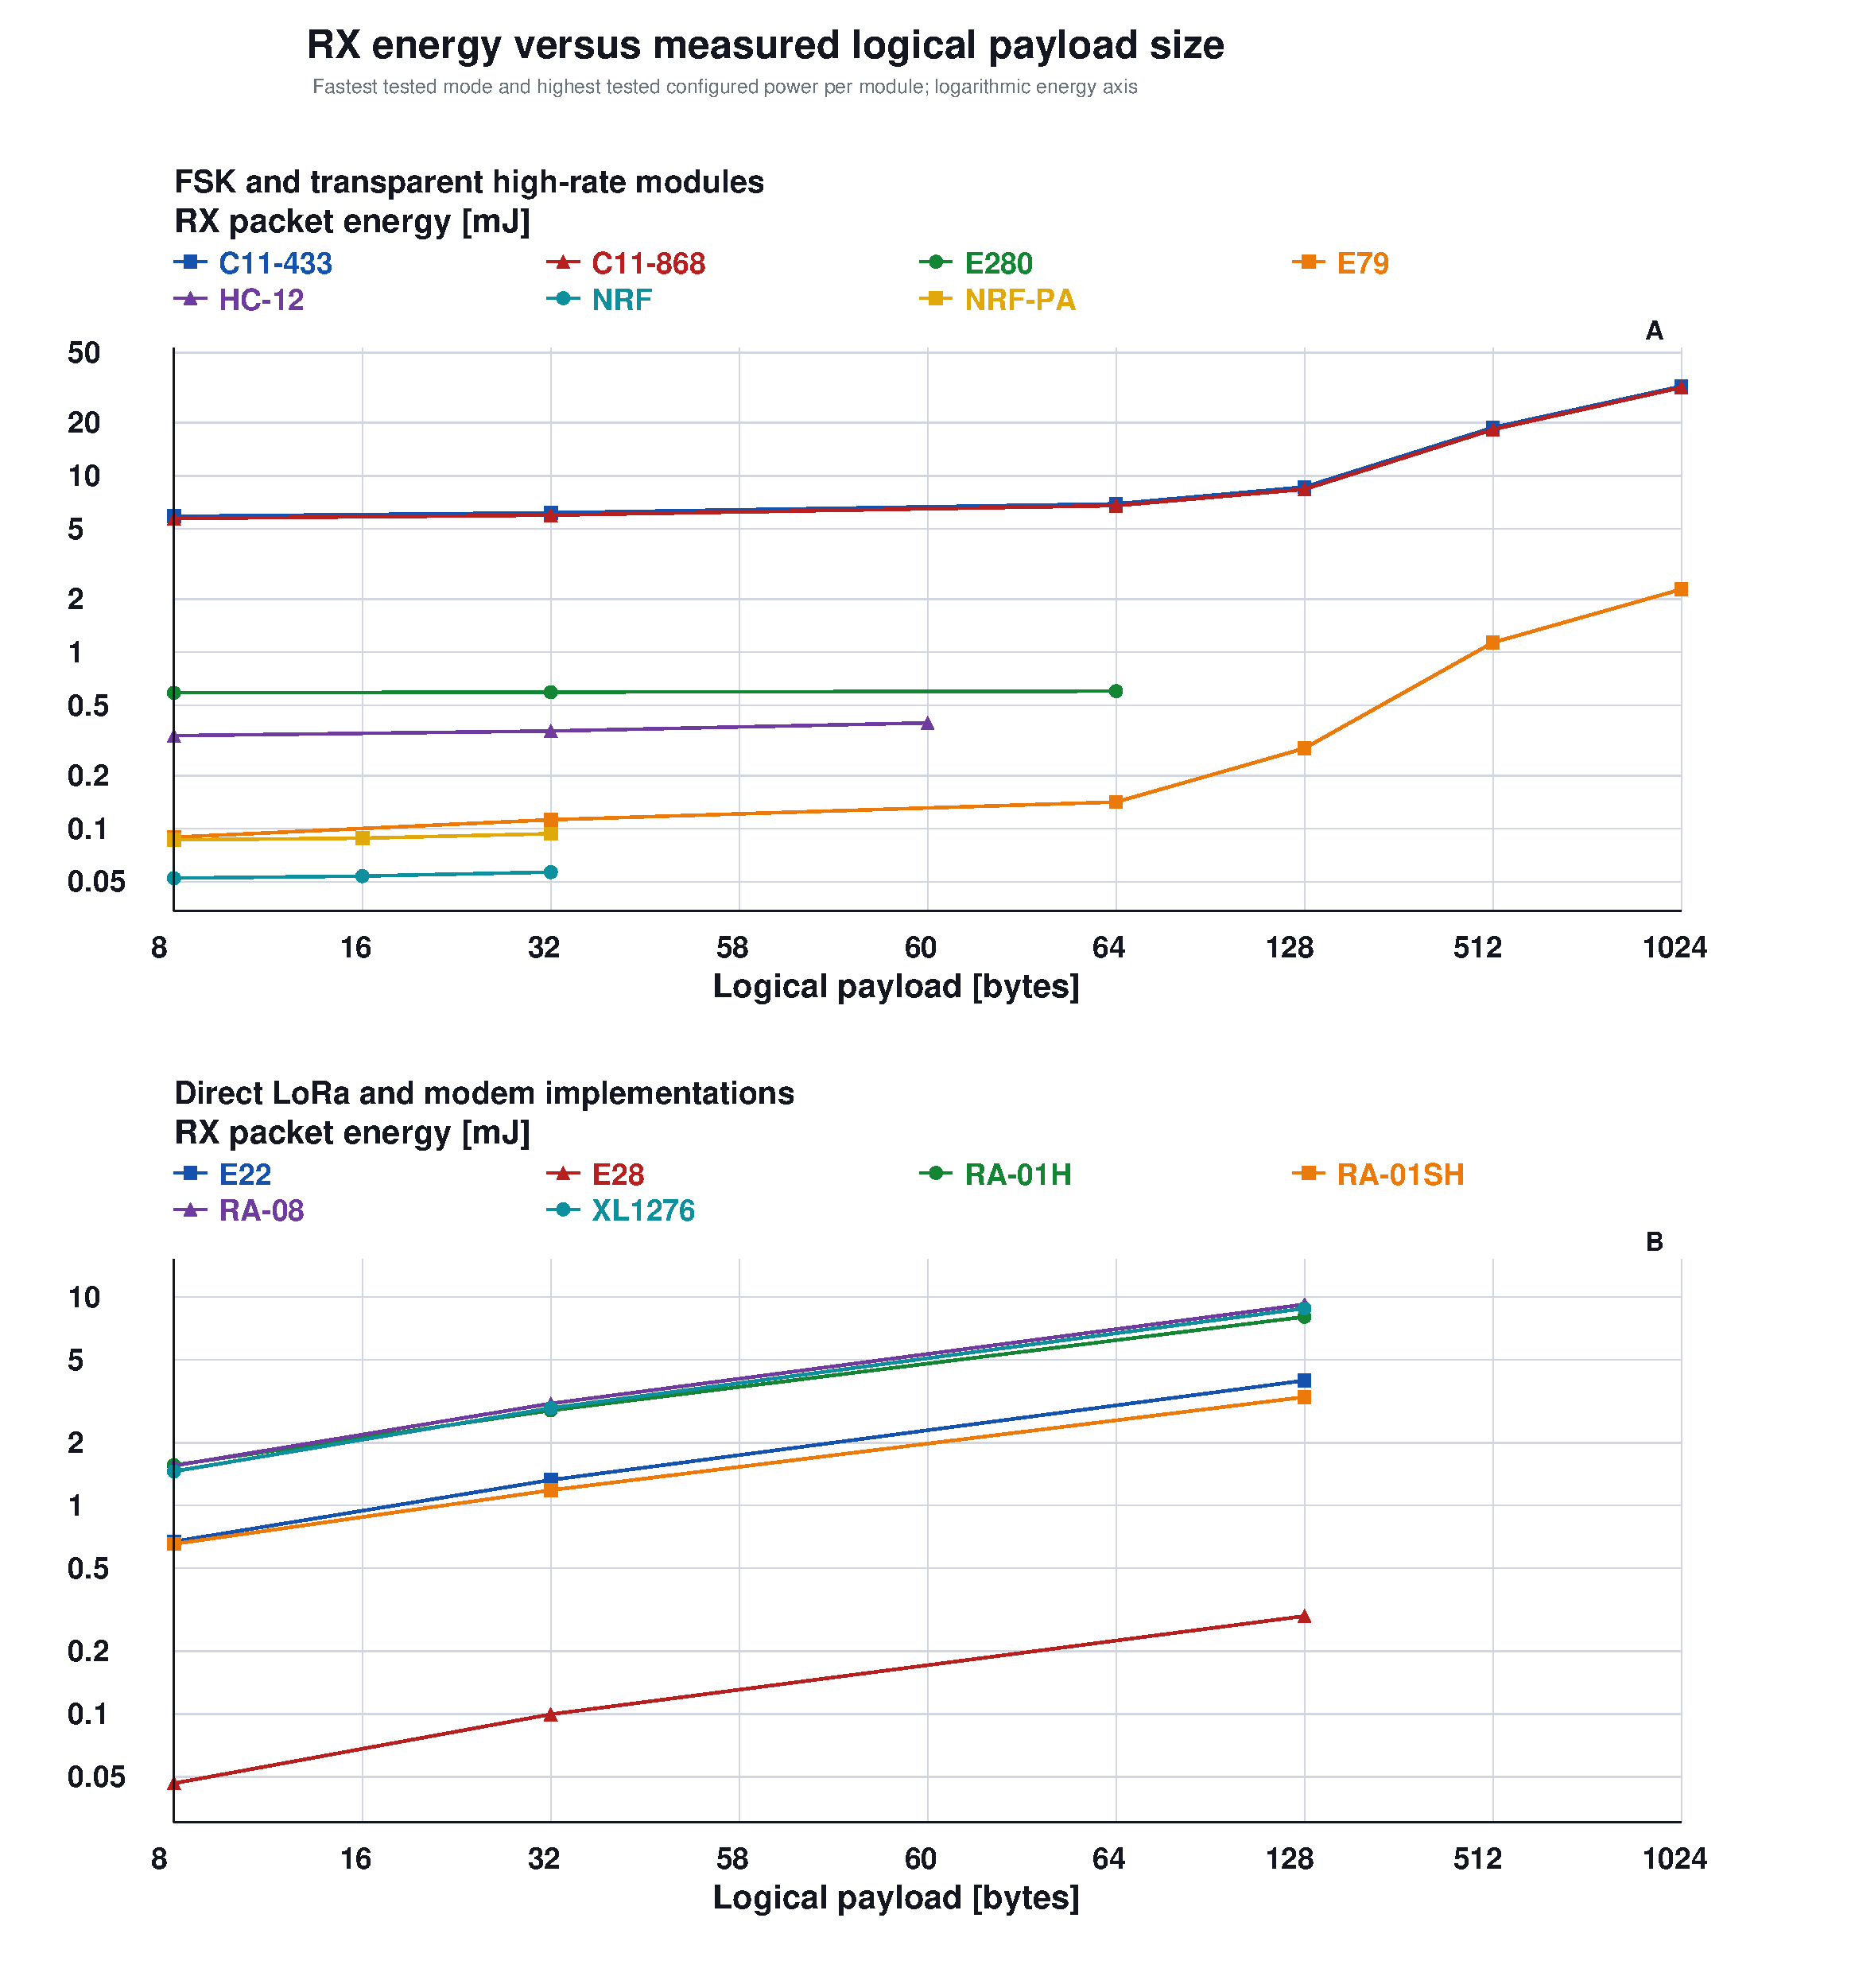
\includegraphics[width=\linewidth]{figures/rx_energy_by_payload.pdf}
  \caption{Measured RX event energy versus logical payload size, panels A--B, under the same per-module mode and configured-power rule as the TX matrix.}
  \label{fig:rx-payload}
\end{figure}

\begin{figure}[p]
  \centering
  \ContinuedFloat
  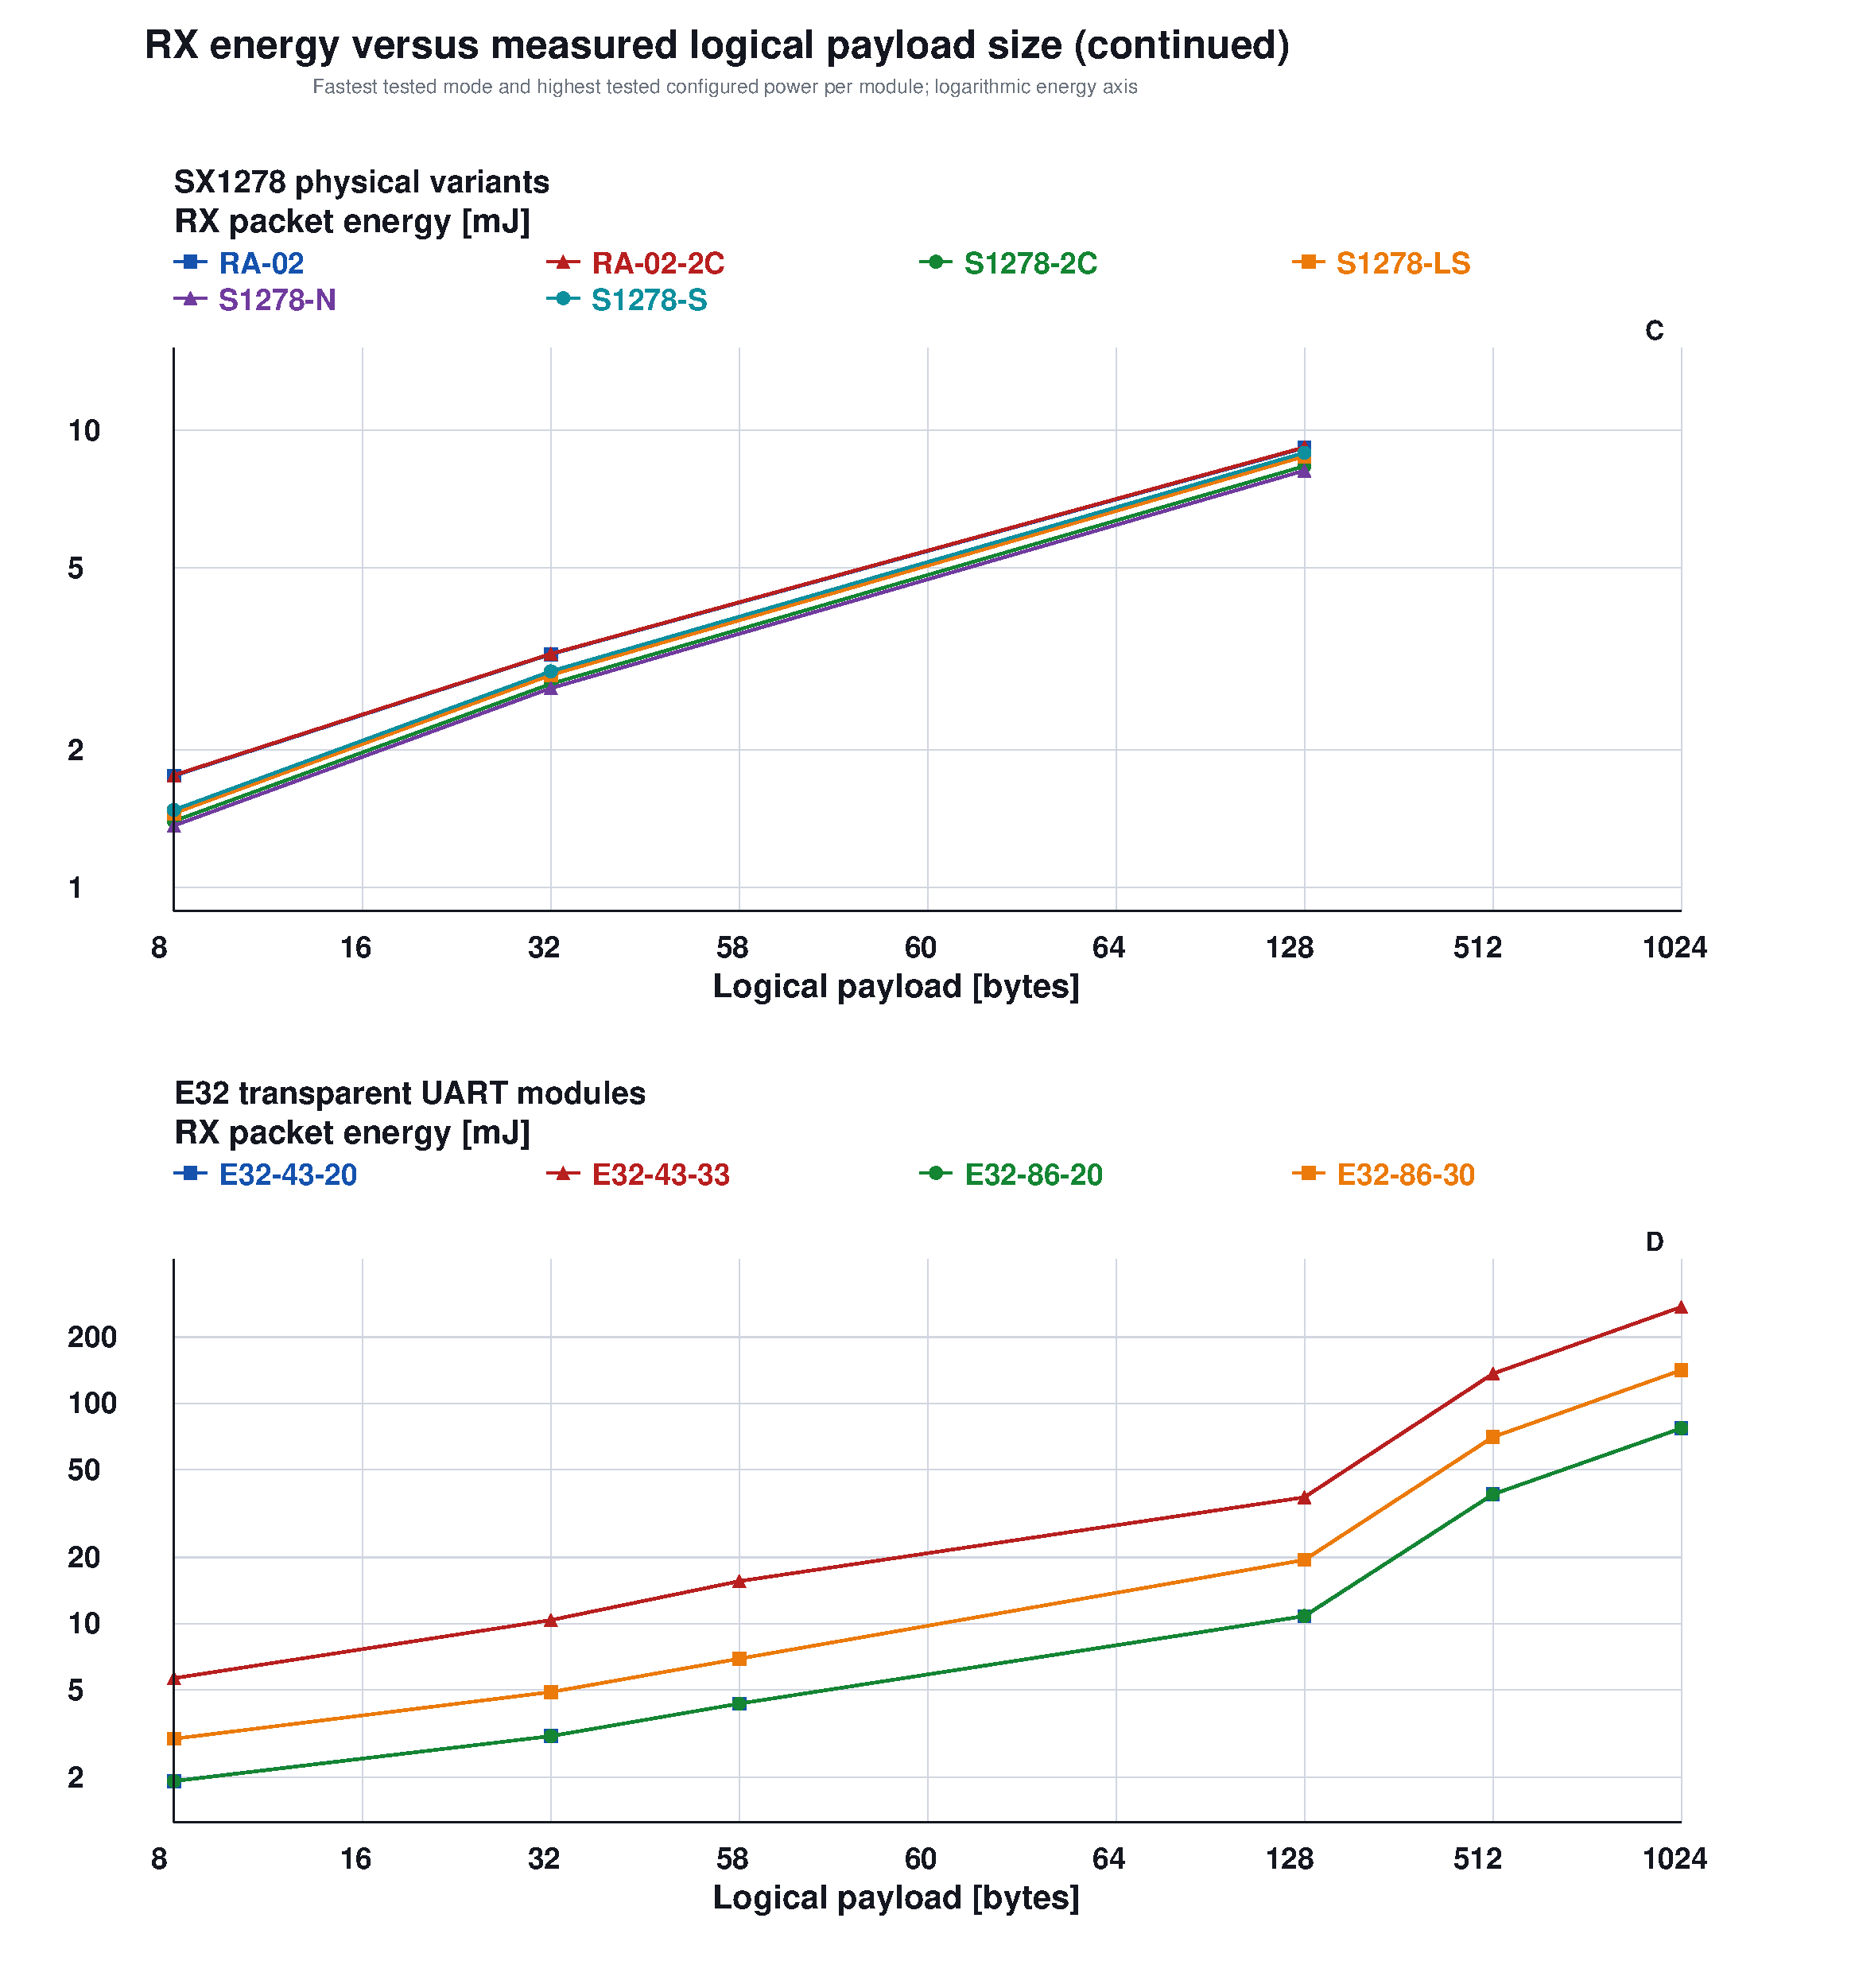
\includegraphics[width=\linewidth]{figures/rx_energy_by_payload_continued.pdf}
  \caption{Measured RX event energy versus logical payload size, panels C--D (continued).}
\end{figure}
\clearpage

Absolute packet energy increases with payload size for every measured TX series. It does not increase in direct proportion to application bytes because each event contains fixed startup, synchronization, command, and receive-window costs. Comparing each module's smallest and largest measured payload, the TX energy per application byte at the largest point falls to 17--57\% of its 8-byte value; the corresponding RX range is 4--40\%. These ranges summarize different payload limits and must not be interpreted as equal-size rankings.

The long-payload campaigns make the practical scale visible. E79/GFSK200 rises from \SI{0.0757}{mJ} at 8 bytes to \SI{1.660}{mJ} at 1024 bytes: a 128-fold payload increase costs 21.9 times more event energy. The E32-433T33D rises from \SI{78.92}{mJ} to \SI{3820.3}{mJ} over the same logical sizes. At the opposite extreme, the nRF24L01 hardware payload ends at 32 bytes; its measured TX event rises only from \SI{0.0125}{mJ} at 8 bytes to \SI{0.0187}{mJ} at 32 bytes. Application messages larger than the tested native payload limit would require a separate multi-packet experiment and are not extrapolated here.

The 58-, 60-, and 64-byte columns are also intentionally separate. They correspond to E32, HC-12, and other campaign-specific boundaries. Likewise, the 128-, 512-, and 1024-byte values are logical-message totals produced by the tested firmware's fragmentation behavior, not single over-the-air frames for every radio. This is precisely why absolute message energy is more useful for battery budgeting than a lone per-bit value.

\subsection{Sustained-traffic power and useful rate}

Table~\ref{tab:benchmark} separates sustained power, delivered goodput, and aggregate delivery from the packet-size matrices. The configured rate and mode columns belong to the selected continuous window. PDR is the aggregate packet delivery ratio; CDR is the aggregate 60-second continuous delivery ratio.

{\scriptsize\setlength{\tabcolsep}{3pt}
\begin{longtable}{@{}llrrrrrrr@{}}
\caption{Sustained-traffic and delivery benchmark. Continuous values use the fastest mode available in each 60-second campaign. PDR and CDR aggregate the complete packet and continuous matrices, respectively.}\label{tab:benchmark}\\
\toprule
ID & Mode & Rate & dBm & $P_{TX}$ & $P_{RX}$ & Goodput & PDR & CDR \\
 & & [kbps] & & [mW] & [mW] & [kbps] & [\%] & [\%] \\ \midrule
\endfirsthead
\toprule ID & Mode & Rate & dBm & $P_{TX}$ & $P_{RX}$ & Goodput & PDR & CDR \\ \midrule
\endhead
C11-433 & 38.4 kbps & 38.40 & 10.00 & 69.58 & 49.77 & 8.572 & 92.5 & 100.0 \\
C11-868 & 38.4 kbps & 38.40 & 10.00 & 42.65 & 46.48 & 8.892 & 100.0 & 90.2 \\
E28 & SF8 & 16.93 & 13.00 & 69.31 & 20.57 & 9.276 & 100.0 & 98.7 \\
E280 & 100 kbps & 100.0 & 12.00 & 66.23 & 62.94 & 7.374 & 100.0 & 40.3 \\
E22 & SF9 & 1.758 & 18.00 & 191.9 & 18.15 & 0.922 & 93.9 & 74.8 \\
E32-43-20 & 4.8 kbps & 4.800 & 20.00 & 275.9 & 43.44 & 1.687 & 99.7 & 81.0 \\
E32-43-33 & 4.8 kbps & 4.800 & 30.00 & 2524.9 & 202.7 & 1.650 & 83.1 & 59.5 \\
E32-86-20 & 4.8 kbps & 4.800 & 20.00 & 276.4 & 43.44 & 1.687 & 99.7 & 80.9 \\
E32-86-30 & 4.8 kbps & 4.800 & 30.00 & 1377.0 & 72.12 & 1.635 & 100.0 & 81.1 \\
E79 & SLR2K5 & 2.500 & 13.00 & 29.34 & 22.75 & 2.057 & 99.9 & 100.0 \\
HC-12 & 15 kbps & 15.00 & 20.00 & 102.9 & 56.39 & 3.047 & 100.0 & 100.0 \\
NRF & 1000 kbps & 1000.0 & 0 & 1.695 & 41.80 & 11.07 & 78.9 & 86.5 \\
NRF-PA & 1000 kbps & 1000.0 & 0 & 8.980 & 73.30 & 7.987 & 64.4 & 62.2 \\
RA-01H & SF9 & 1.758 & 20.00 & 367.4 & 35.87 & 1.149 & 98.3 & 99.3 \\
RA-01SH & SF9 & 1.758 & 22.00 & 217.1 & 14.76 & 1.186 & 100.0 & 100.0 \\
RA-02 & SF9 & 1.758 & 20.00 & 203.7 & 40.96 & 1.186 & 99.4 & 99.6 \\
RA-02-2C & SF9 & 1.758 & 20.00 & 196.9 & 41.07 & 1.178 & 99.4 & 99.4 \\
RA-08 & SF9 & 1.758 & 22.00 & 415.4 & 42.40 & 1.212 & 100.0 & 100.0 \\
S1278-LS & SF9 & 1.758 & 20.00 & 255.3 & 40.63 & 0.922 & 88.9 & 75.4 \\
S1278-N & SF9 & 1.758 & 20.00 & 240.6 & 37.75 & 1.169 & 99.4 & 70.5 \\
S1278-2C & SF9 & 1.758 & 20.00 & 237.7 & 38.58 & 1.169 & 85.0 & 65.9 \\
S1278-S & SF9 & 1.758 & 20.00 & 244.1 & 41.37 & 0.93 & 98.9 & 76.9 \\
XL1276 & SF9 & 1.758 & 20.00 & 282.9 & 40.78 & 1.246 & 100.0 & 98.9 \\
\bottomrule
\end{longtable}

}

\begin{figure}[htbp]
  \centering
  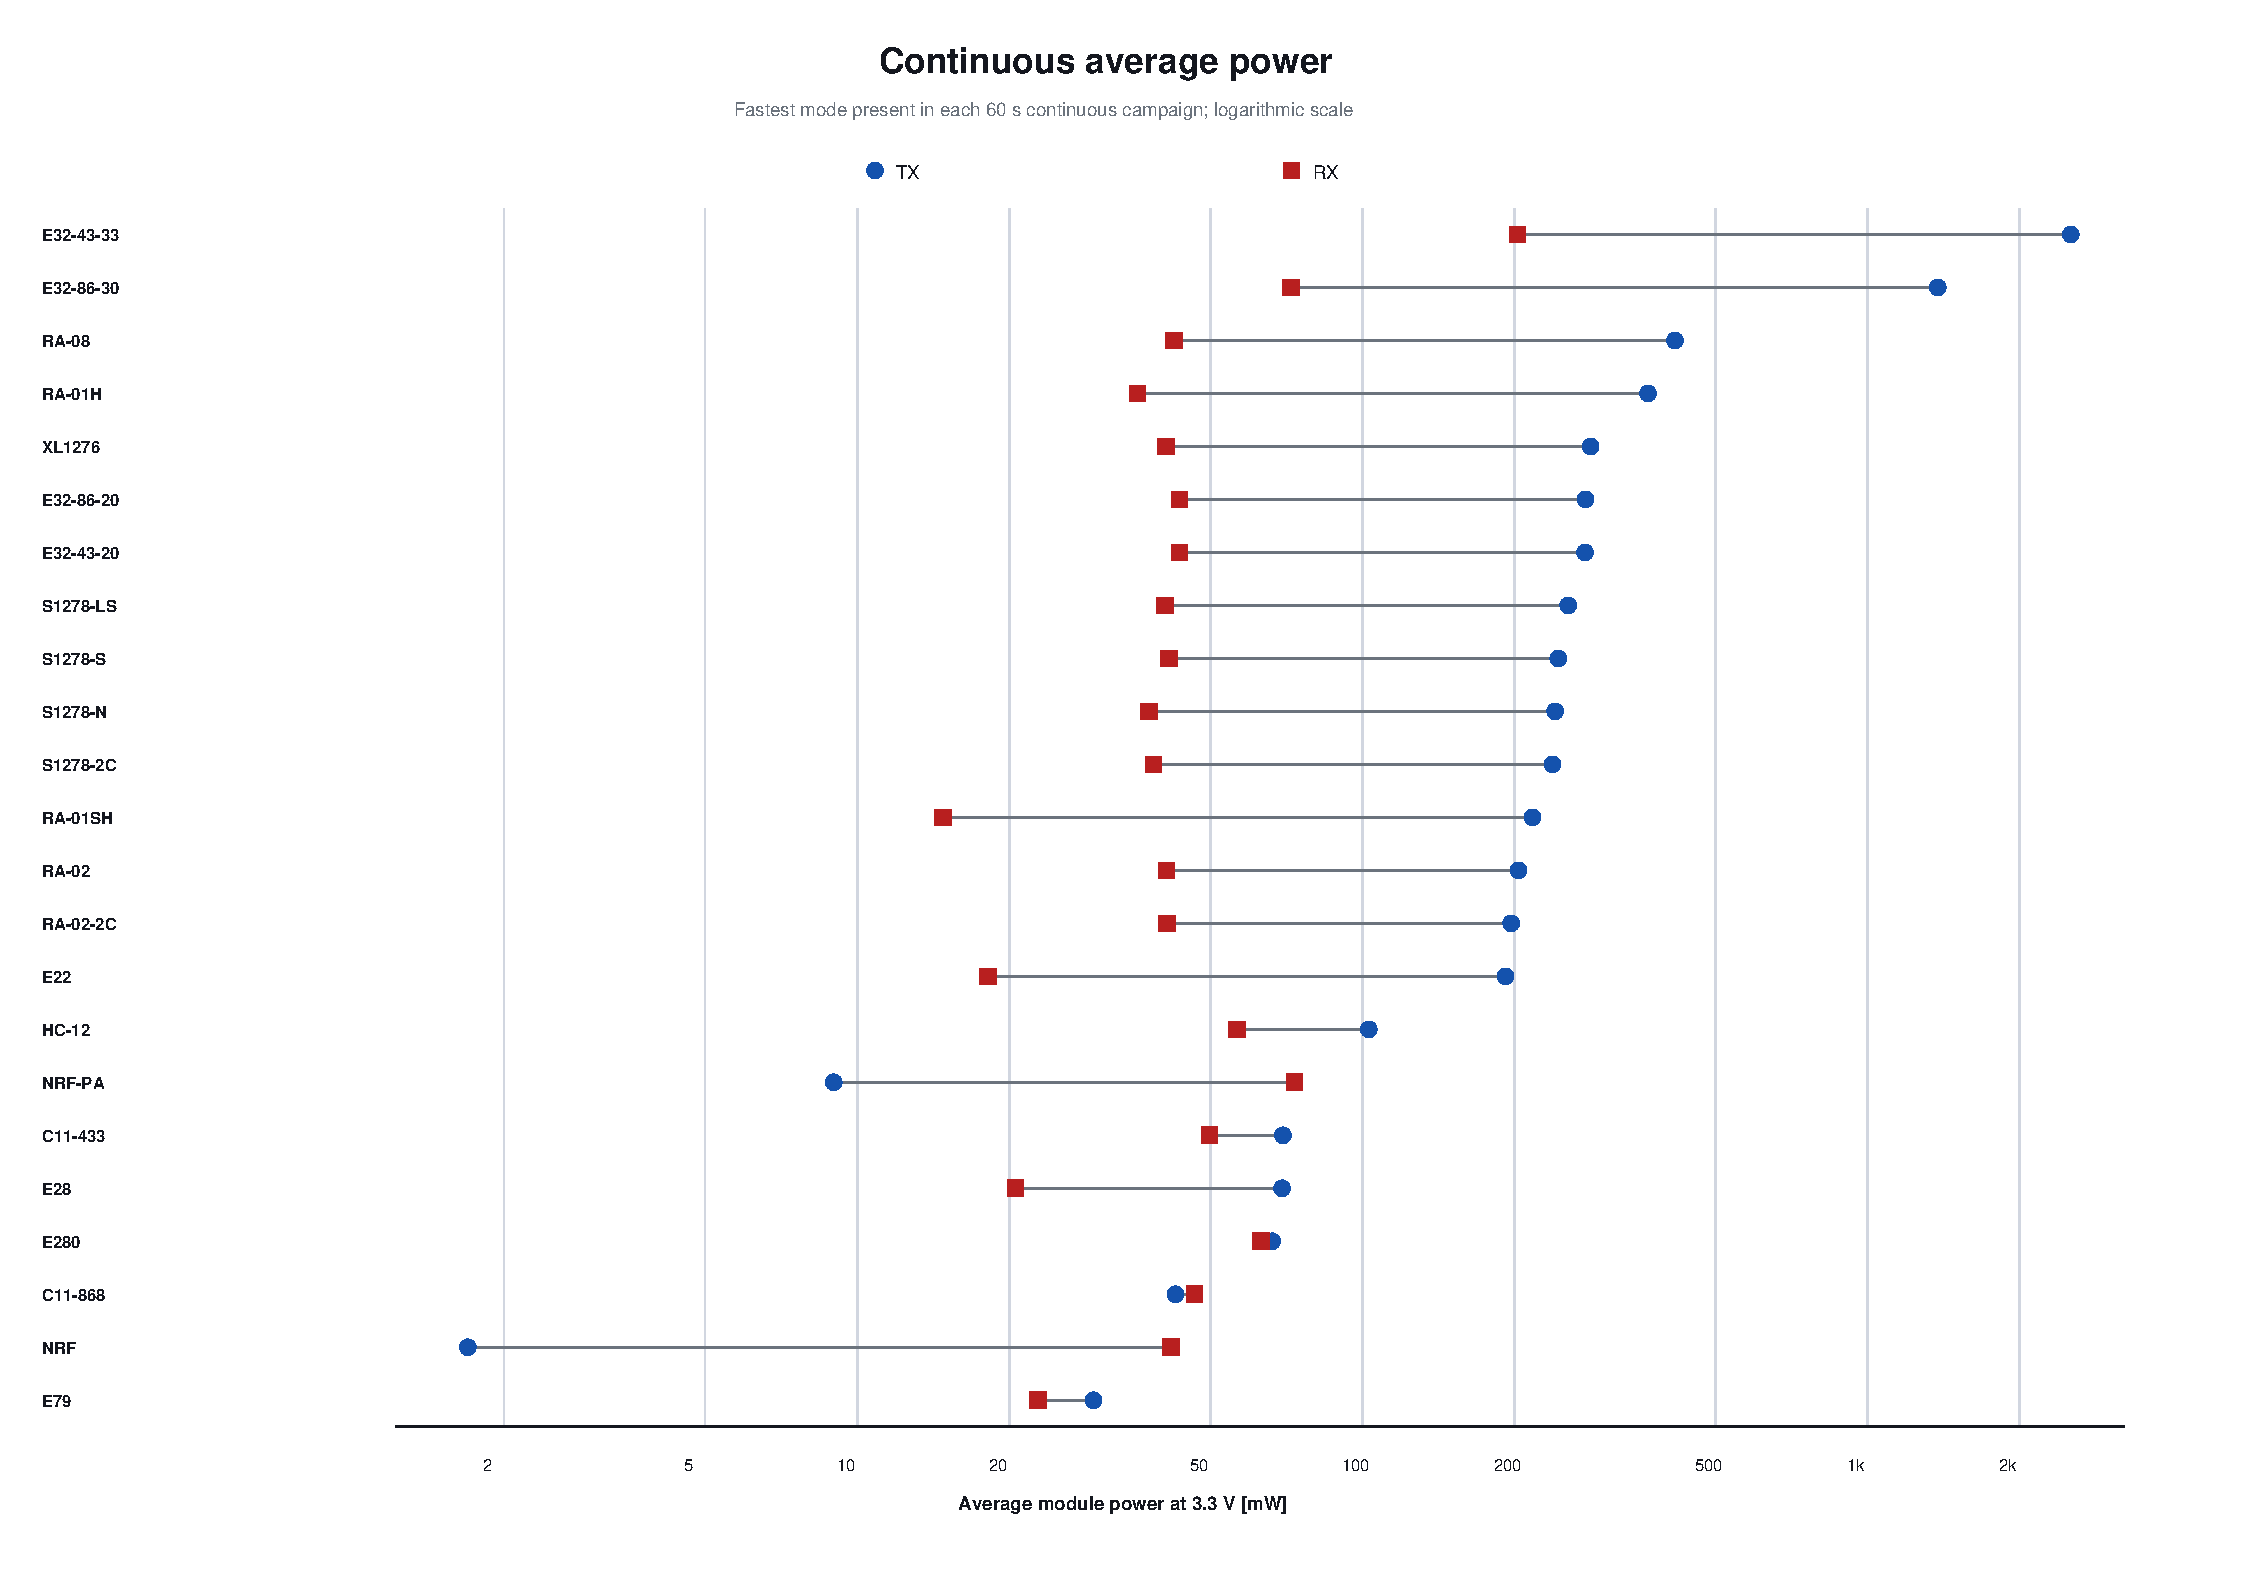
\includegraphics[width=\linewidth]{figures/continuous_power_comparison.pdf}
  \caption{Average module power during the selected 60-second host-driven traffic window. TX and RX use the same mode and configured power within each module.}
  \label{fig:continuous-power}
\end{figure}

The minimum selected TX average is \SI{\LowestTxPower}{mW} for \LowestTxModule, while the E32-433T33D reaches approximately \SI{2.525}{W}. The low nRF24L01 value reflects brief transmissions and idle gaps rather than a permanently enabled carrier. On RX, \LowestRxModule{} is lowest at \SI{\LowestRxPower}{mW}; this agrees directionally with the lower active-RX architecture of the SX1262 generation, whose vendor specification lists a substantially lower receiver current than the SX1276 generation \cite{semtech_sx1262,semtech_sx1276}.

The highest measured useful goodput in the selected matched windows is \SI{\HighestGoodput}{kbps} for \HighestGoodputModule. This is far below the radio's configured \SI{1}{Mbps} rate because the workload includes a fixed host gap and framing. The result is therefore useful for this bridge and firmware stack, but not a statement about the maximum ESB PHY throughput.

\begin{figure}[htbp]
  \centering
  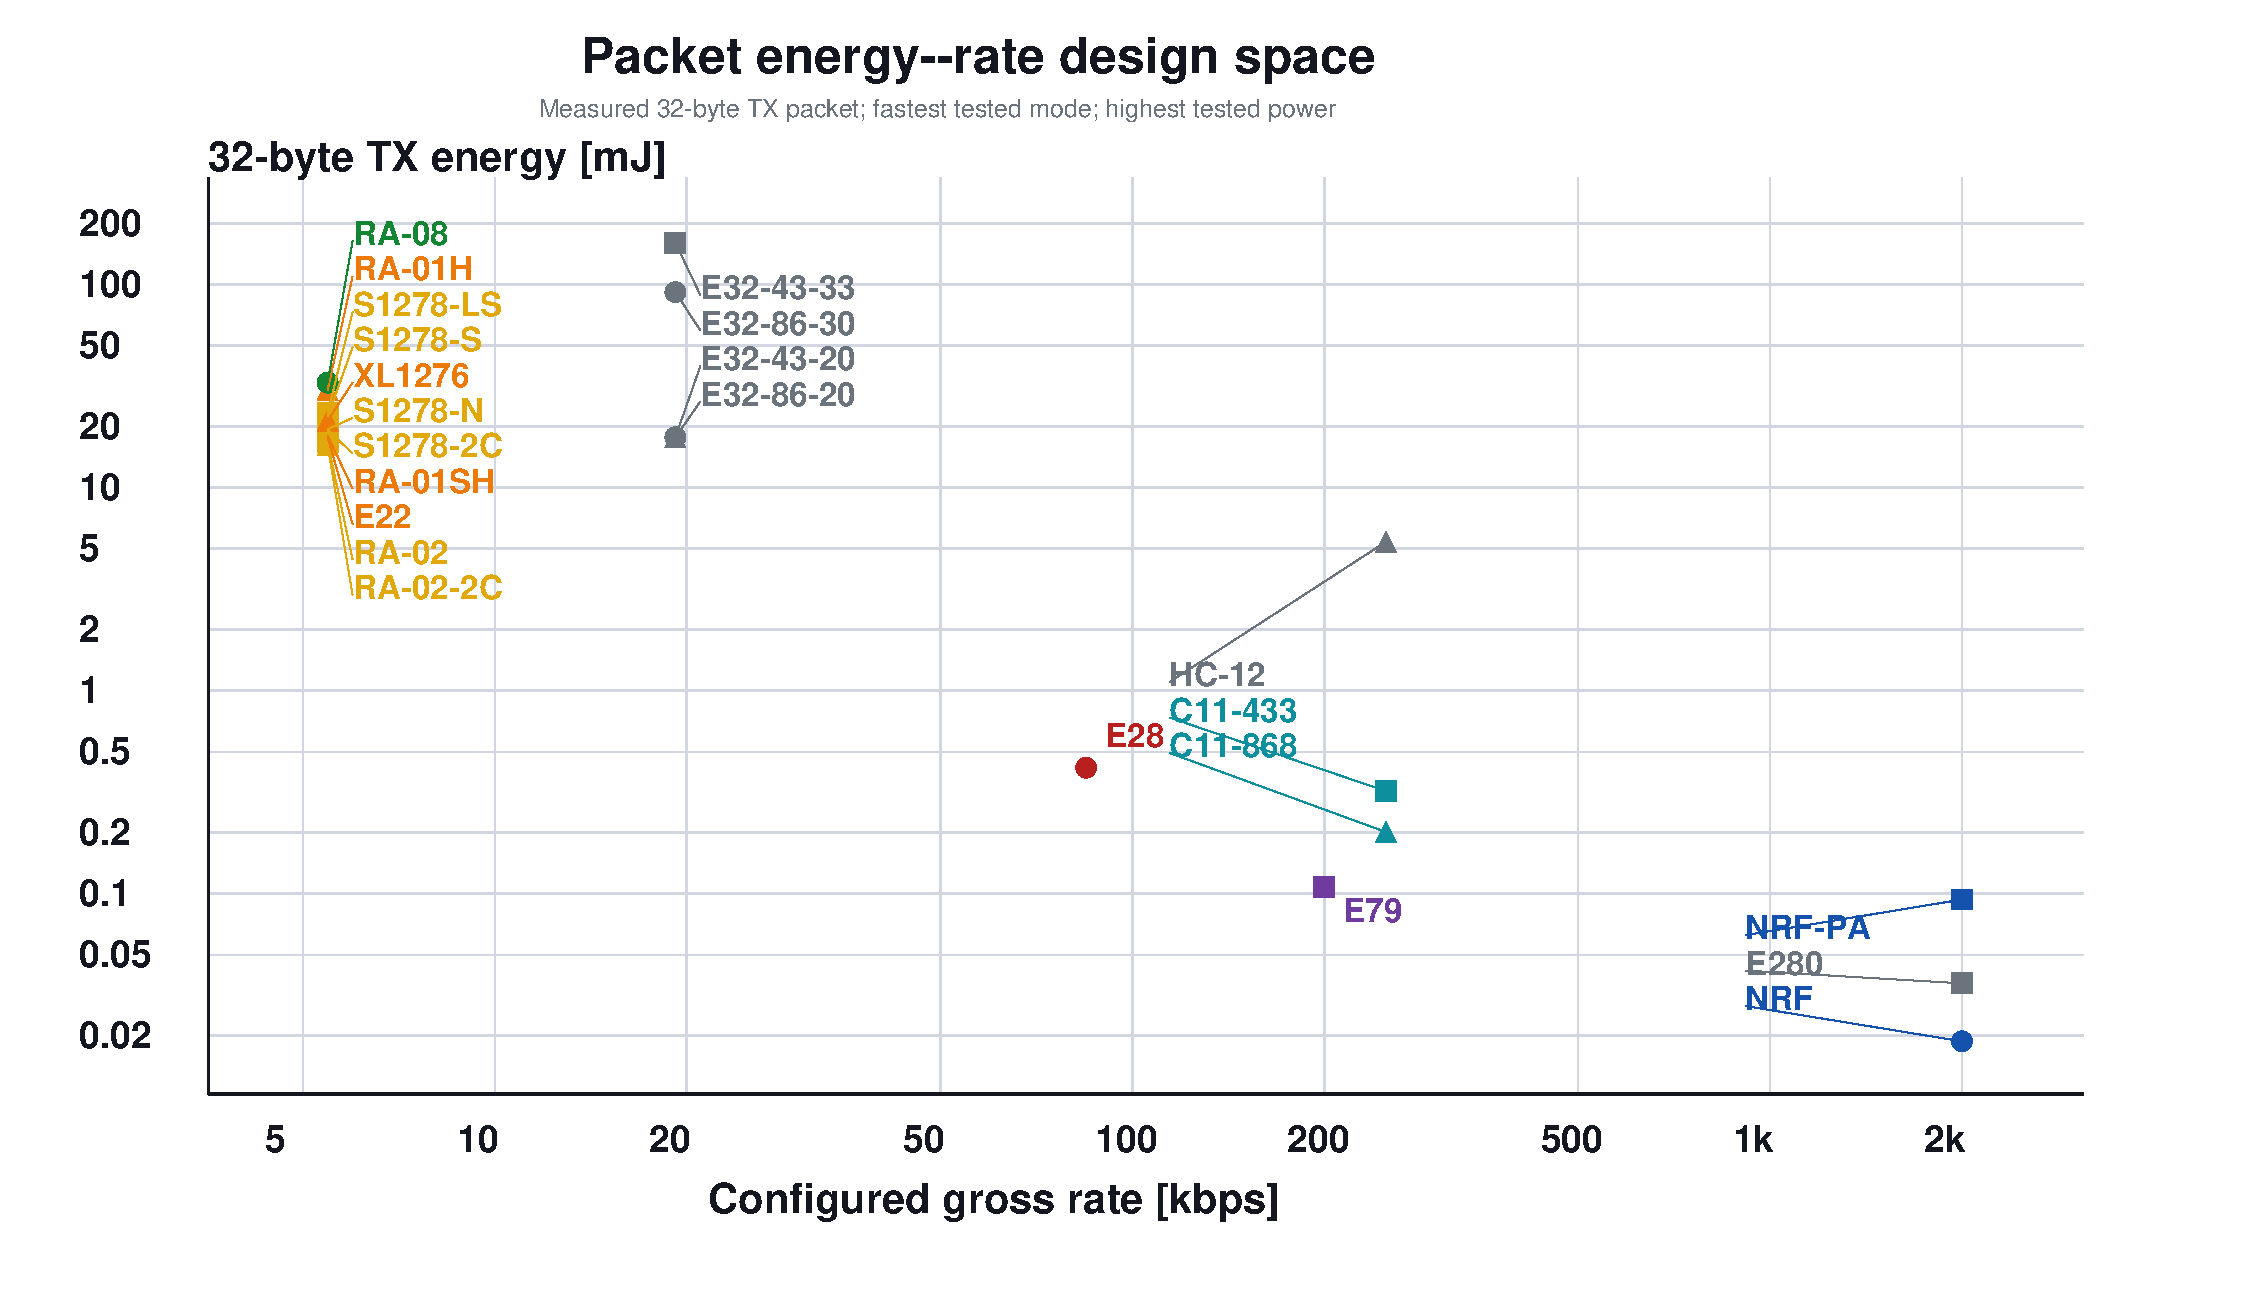
\includegraphics[width=\linewidth]{figures/rate_energy_design_space.pdf}
  \caption{Configured packet-mode rate versus measured TX energy for one 32-byte application packet. Points farther right and lower are preferable for this short-range workload, but the plot does not encode sensitivity, range, interference tolerance, or regulatory limits.}
  \label{fig:design-space}
\end{figure}

The design space separates into visible regimes. The \SI{2.4}{GHz} GFSK/transparent devices occupy the high-rate, low-energy region; E79 and CC1101 bridge the middle; LoRa SF7/BW125 modules occupy the lower-rate region; high-power transparent E32 variants pay the largest energy cost. LoRa's purpose is robust long-range reception rather than minimum energy at a short bench distance, so Figure~\ref{fig:design-space} must not be read as a range-normalized ranking.

\subsection{Delivery behavior}

\begin{figure}[htbp]
  \centering
  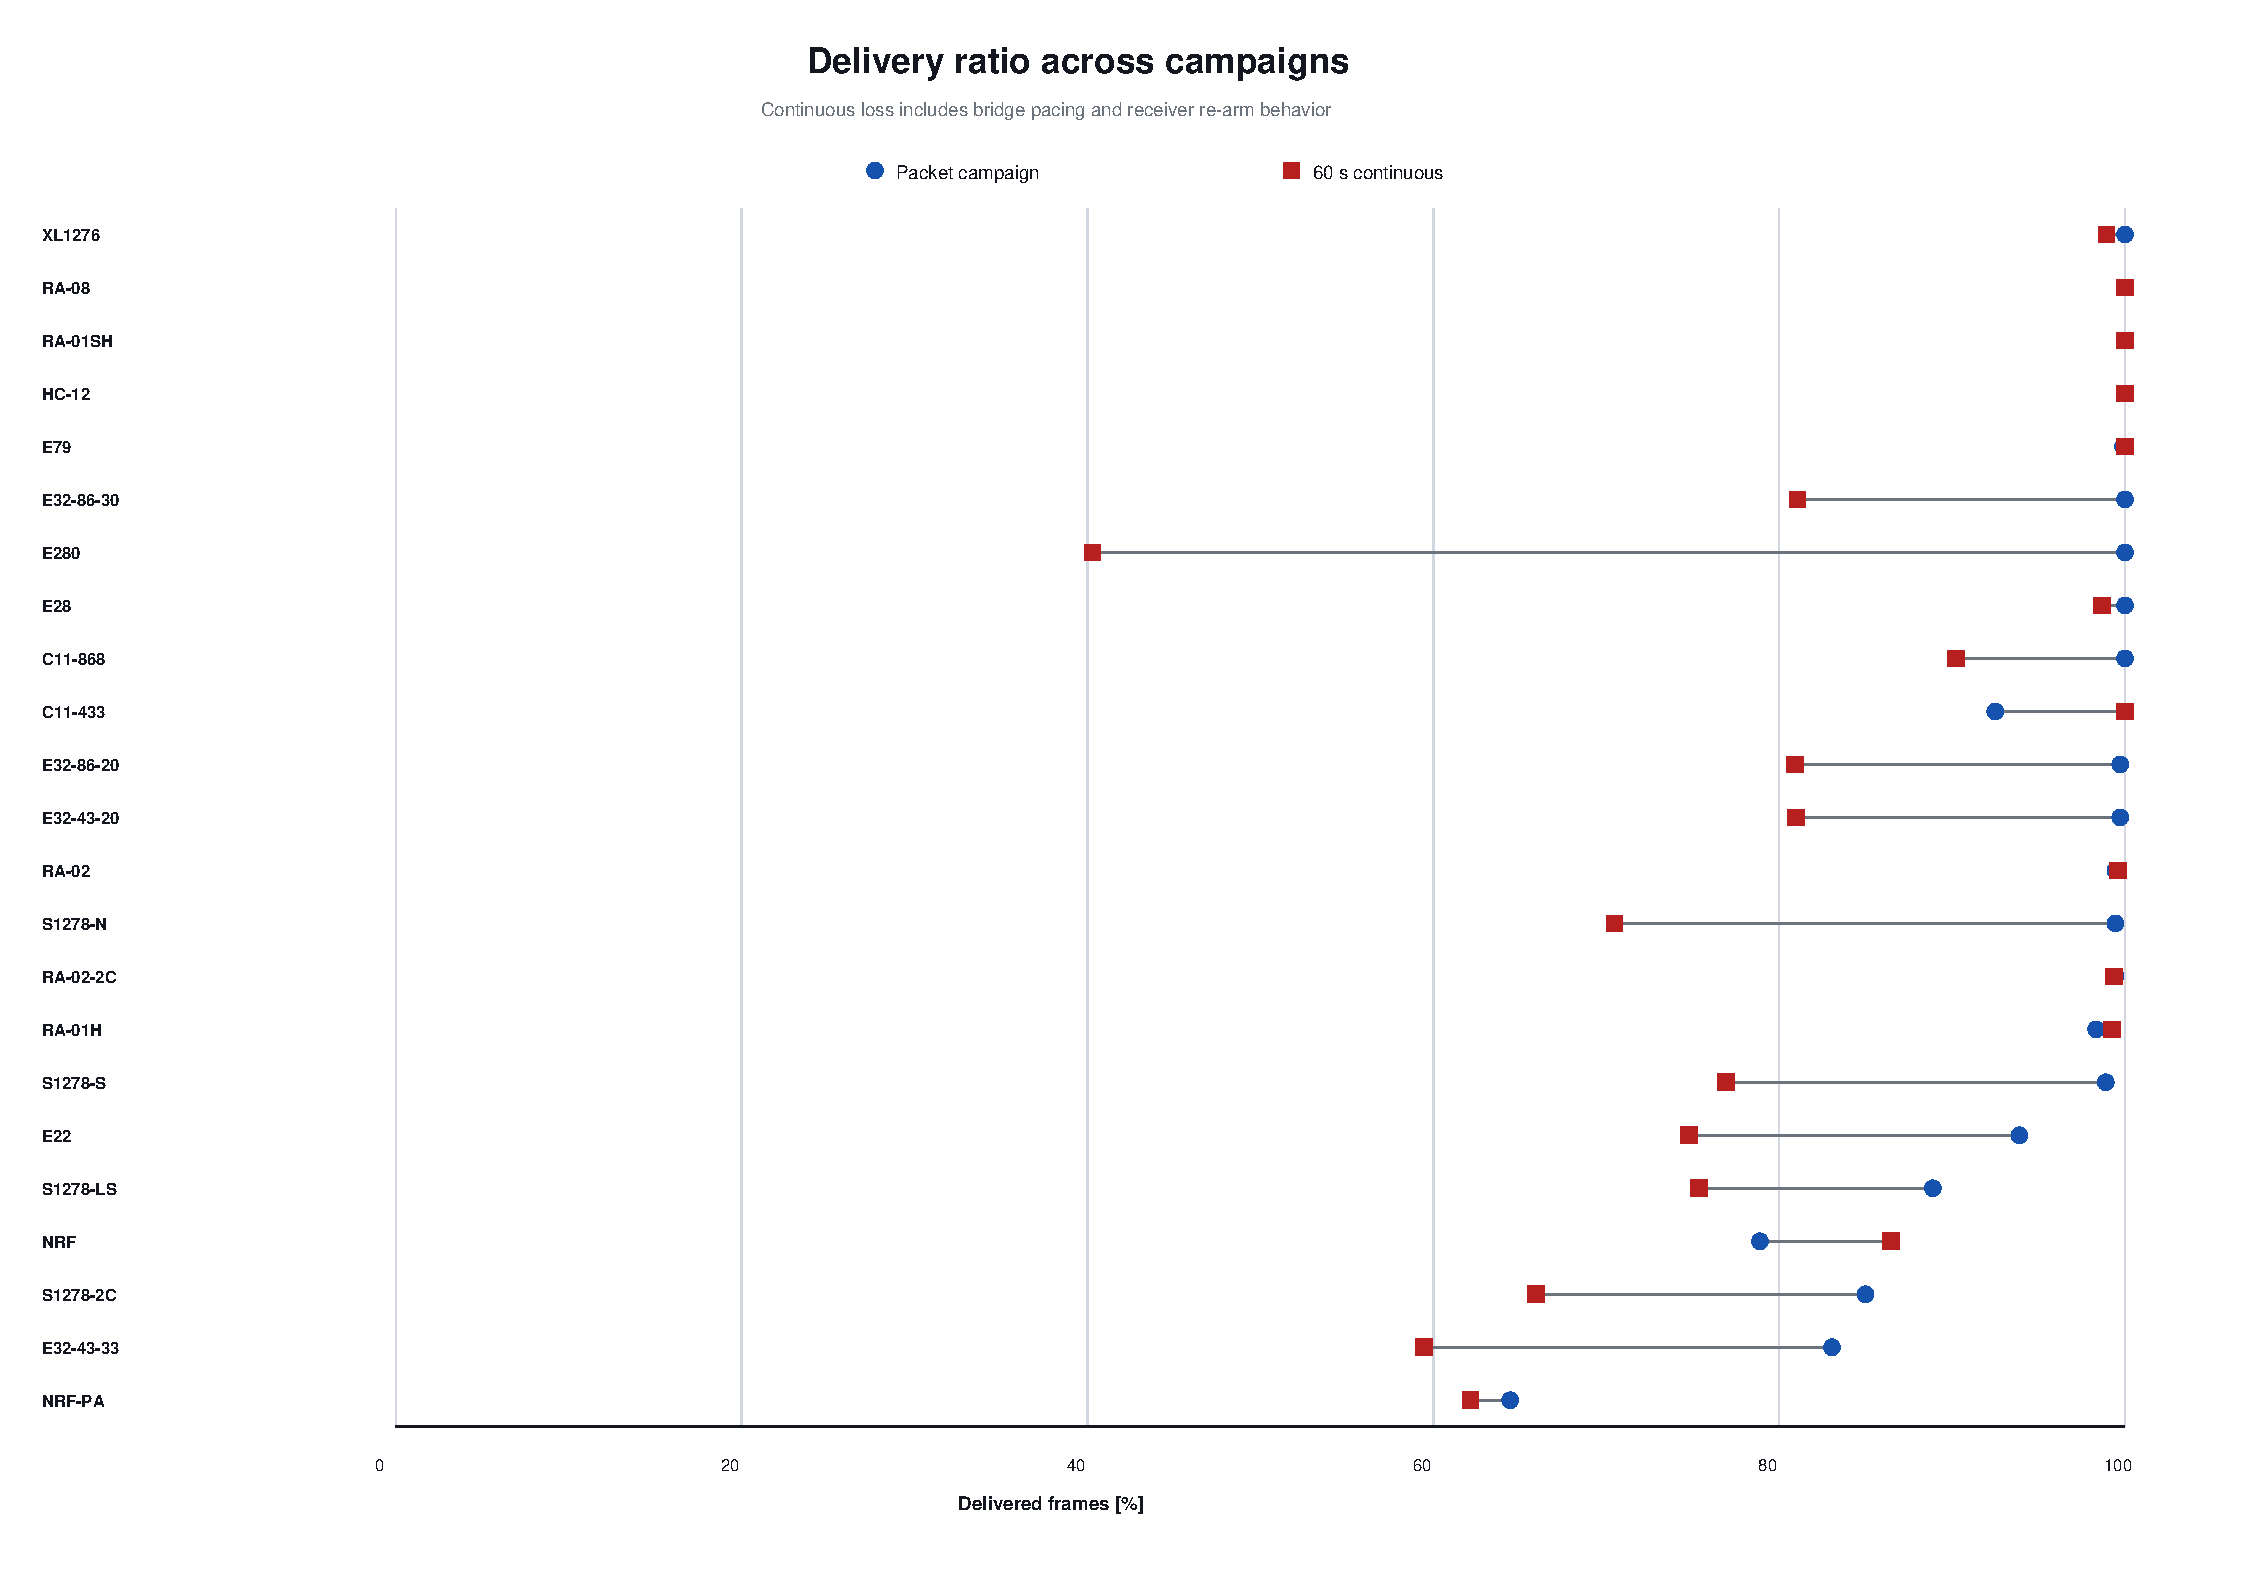
\includegraphics[width=\linewidth]{figures/delivery_comparison.pdf}
  \caption{Aggregate packet and continuous delivery ratios. The continuous ratio is an end-to-end bridge/modem/receiver result and is not a packet-error-rate sensitivity test.}
  \label{fig:delivery}
\end{figure}

Most packet campaigns exceed \SI{98}{\percent}, but several hardware/settings combinations are lower: nRF24L01+PA/LNA (\SI{64.4}{\percent}), nRF24L01 (\SI{78.9}{\percent}), E32-433T33D (\SI{83.1}{\percent}), SX1278 PCB + 2 capacitors (\SI{85.0}{\percent}), and the level-shifter SX1278 board (\SI{88.9}{\percent}). The campaign audits retain these observations because sample loss was not sufficient to explain them.

Continuous delivery is often lower than packet delivery. The E280 reaches only \SI{40.3}{\percent} over its full continuous matrix despite complete packet delivery. Prior controlled checks in the campaign artifacts show that additional receiver/host gap can dramatically reduce loss for slow LoRa configurations. Thus, the continuous metric answers ``how did this complete test stack sustain traffic?'' rather than ``what is the intrinsic RF PER at a specified input level?''

\subsection{E79 multi-PHY comparison}

\begin{figure}[htbp]
  \centering
  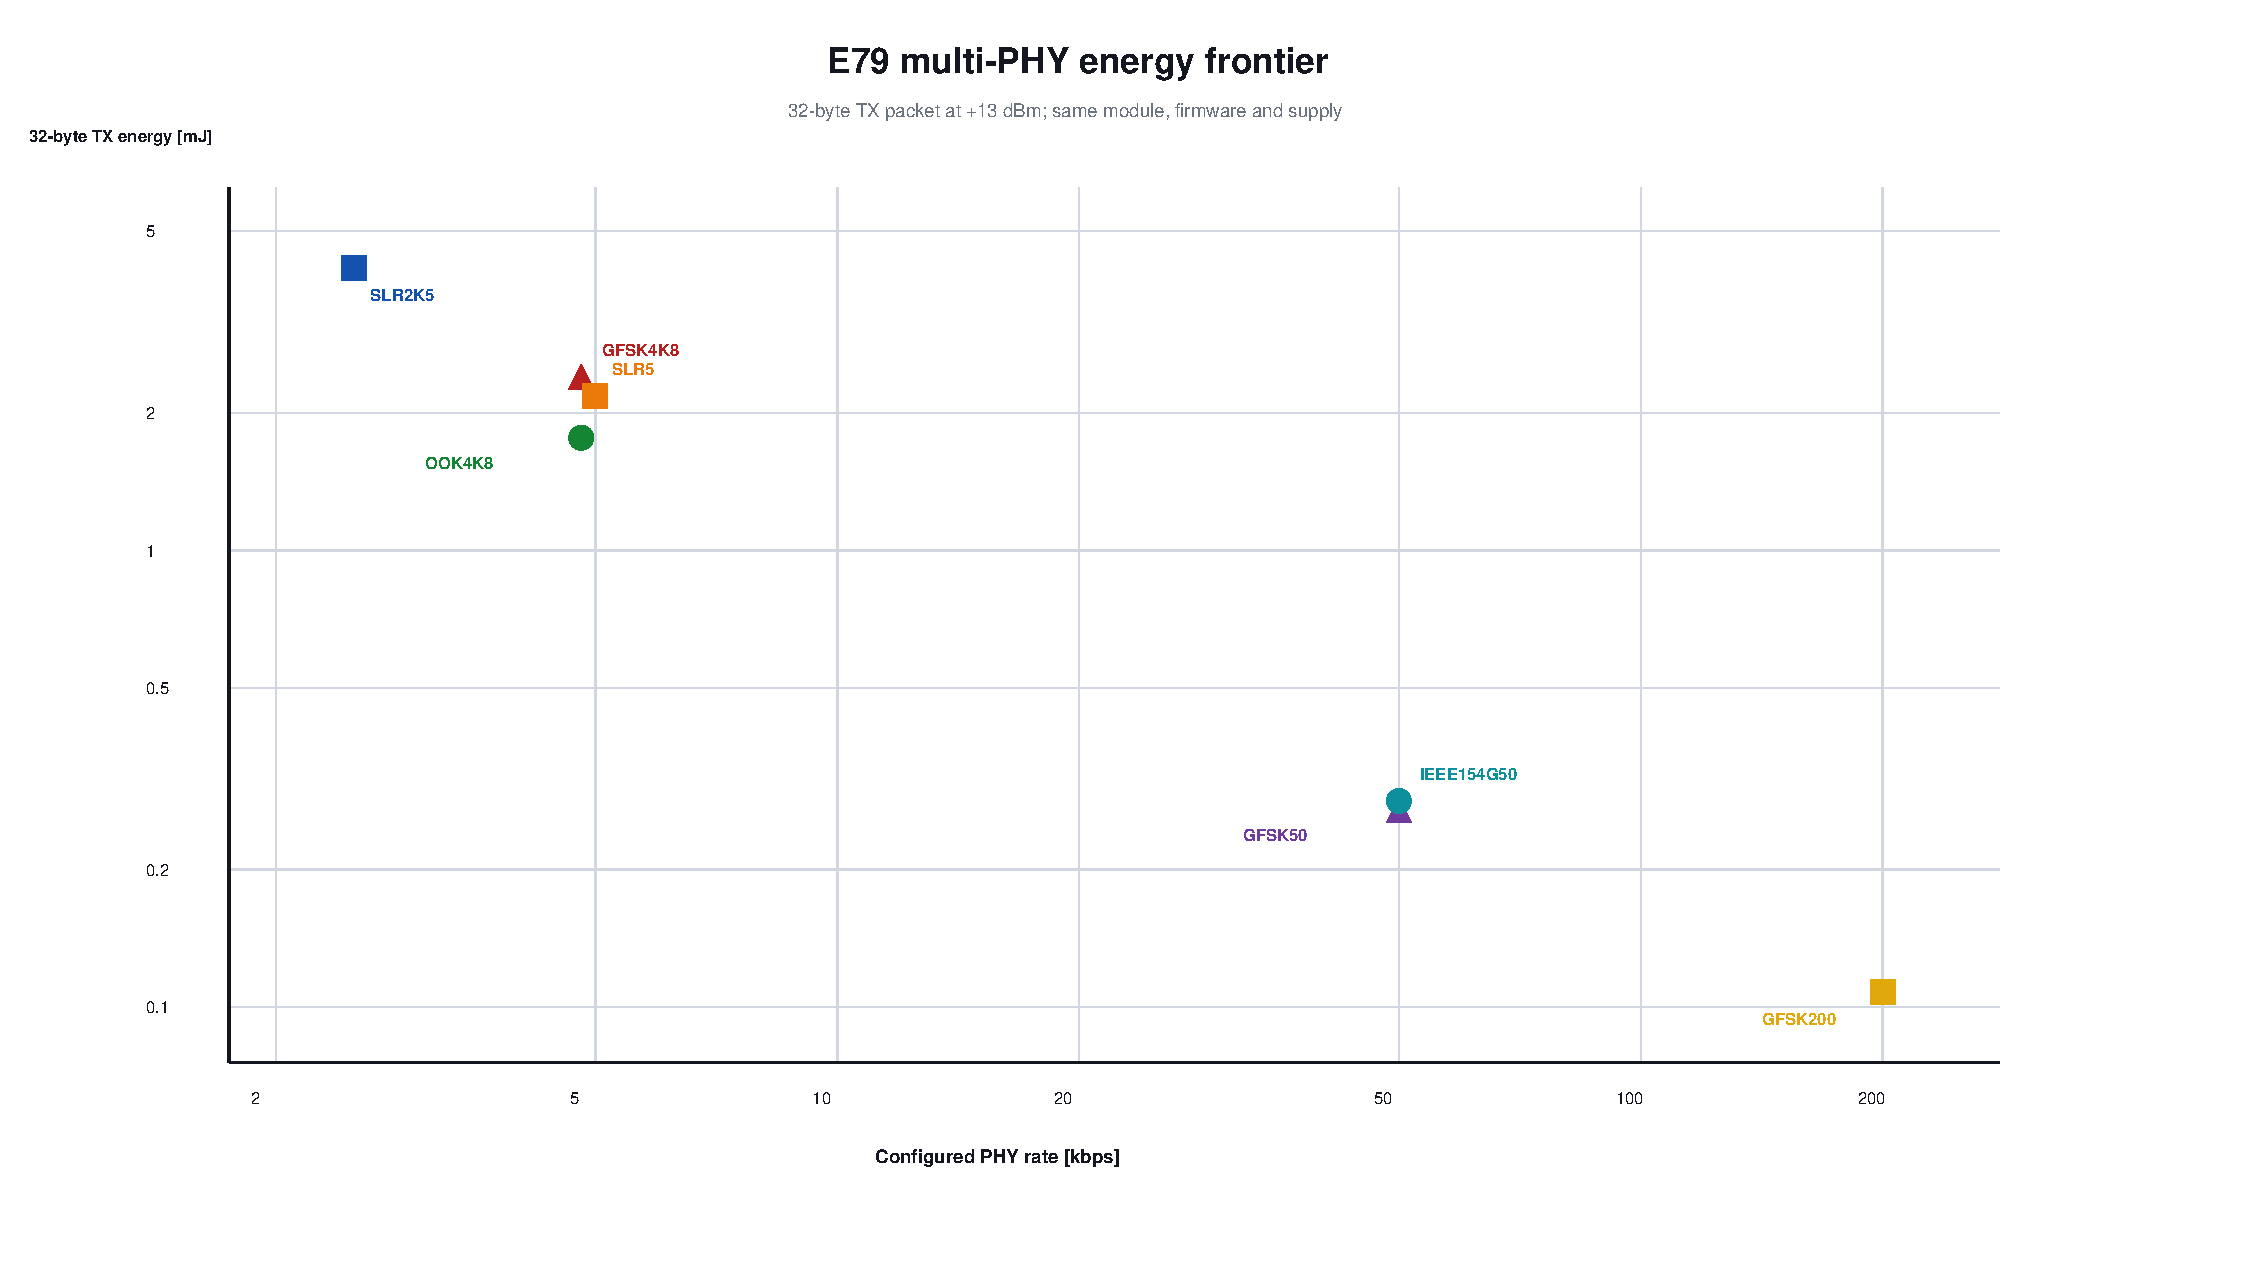
\includegraphics[width=\linewidth]{figures/e79_profile_frontier.pdf}
  \caption{Seven E79/CC1352P PHY profiles on the same module at +13 dBm. This is the cleanest within-device isolation of PHY rate and modulation in the campaign.}
  \label{fig:e79}
\end{figure}

The E79 result provides the strongest evidence that airtime is a first-order energy term. A measured 32-byte GFSK200 transmission requires \SI{\ESeventyNineFastEnergy}{mJ}, while SLR2K5 requires \SI{\ESeventyNineSlowEnergy}{mJ}, a \ESeventyNineImprovement-fold difference on the same hardware, payload, supply, and power setting. At the shared \SI{4.8}{kbps} nominal rate, OOK4K8 uses \SI{1.763}{mJ} and GFSK4K8 uses \SI{2.399}{mJ}. At \SI{50}{kbps}, GFSK50 and IEEE154G50 are close at \SI{0.270}{mJ} and \SI{0.283}{mJ}. Energy alone cannot select among them: SLR trades airtime for coding gain and robustness, while IEEE 802.15.4g and GFSK differ in framing and interoperability.

\subsection{CC1101 revision and band comparison}

\begin{figure}[p]
  \centering
  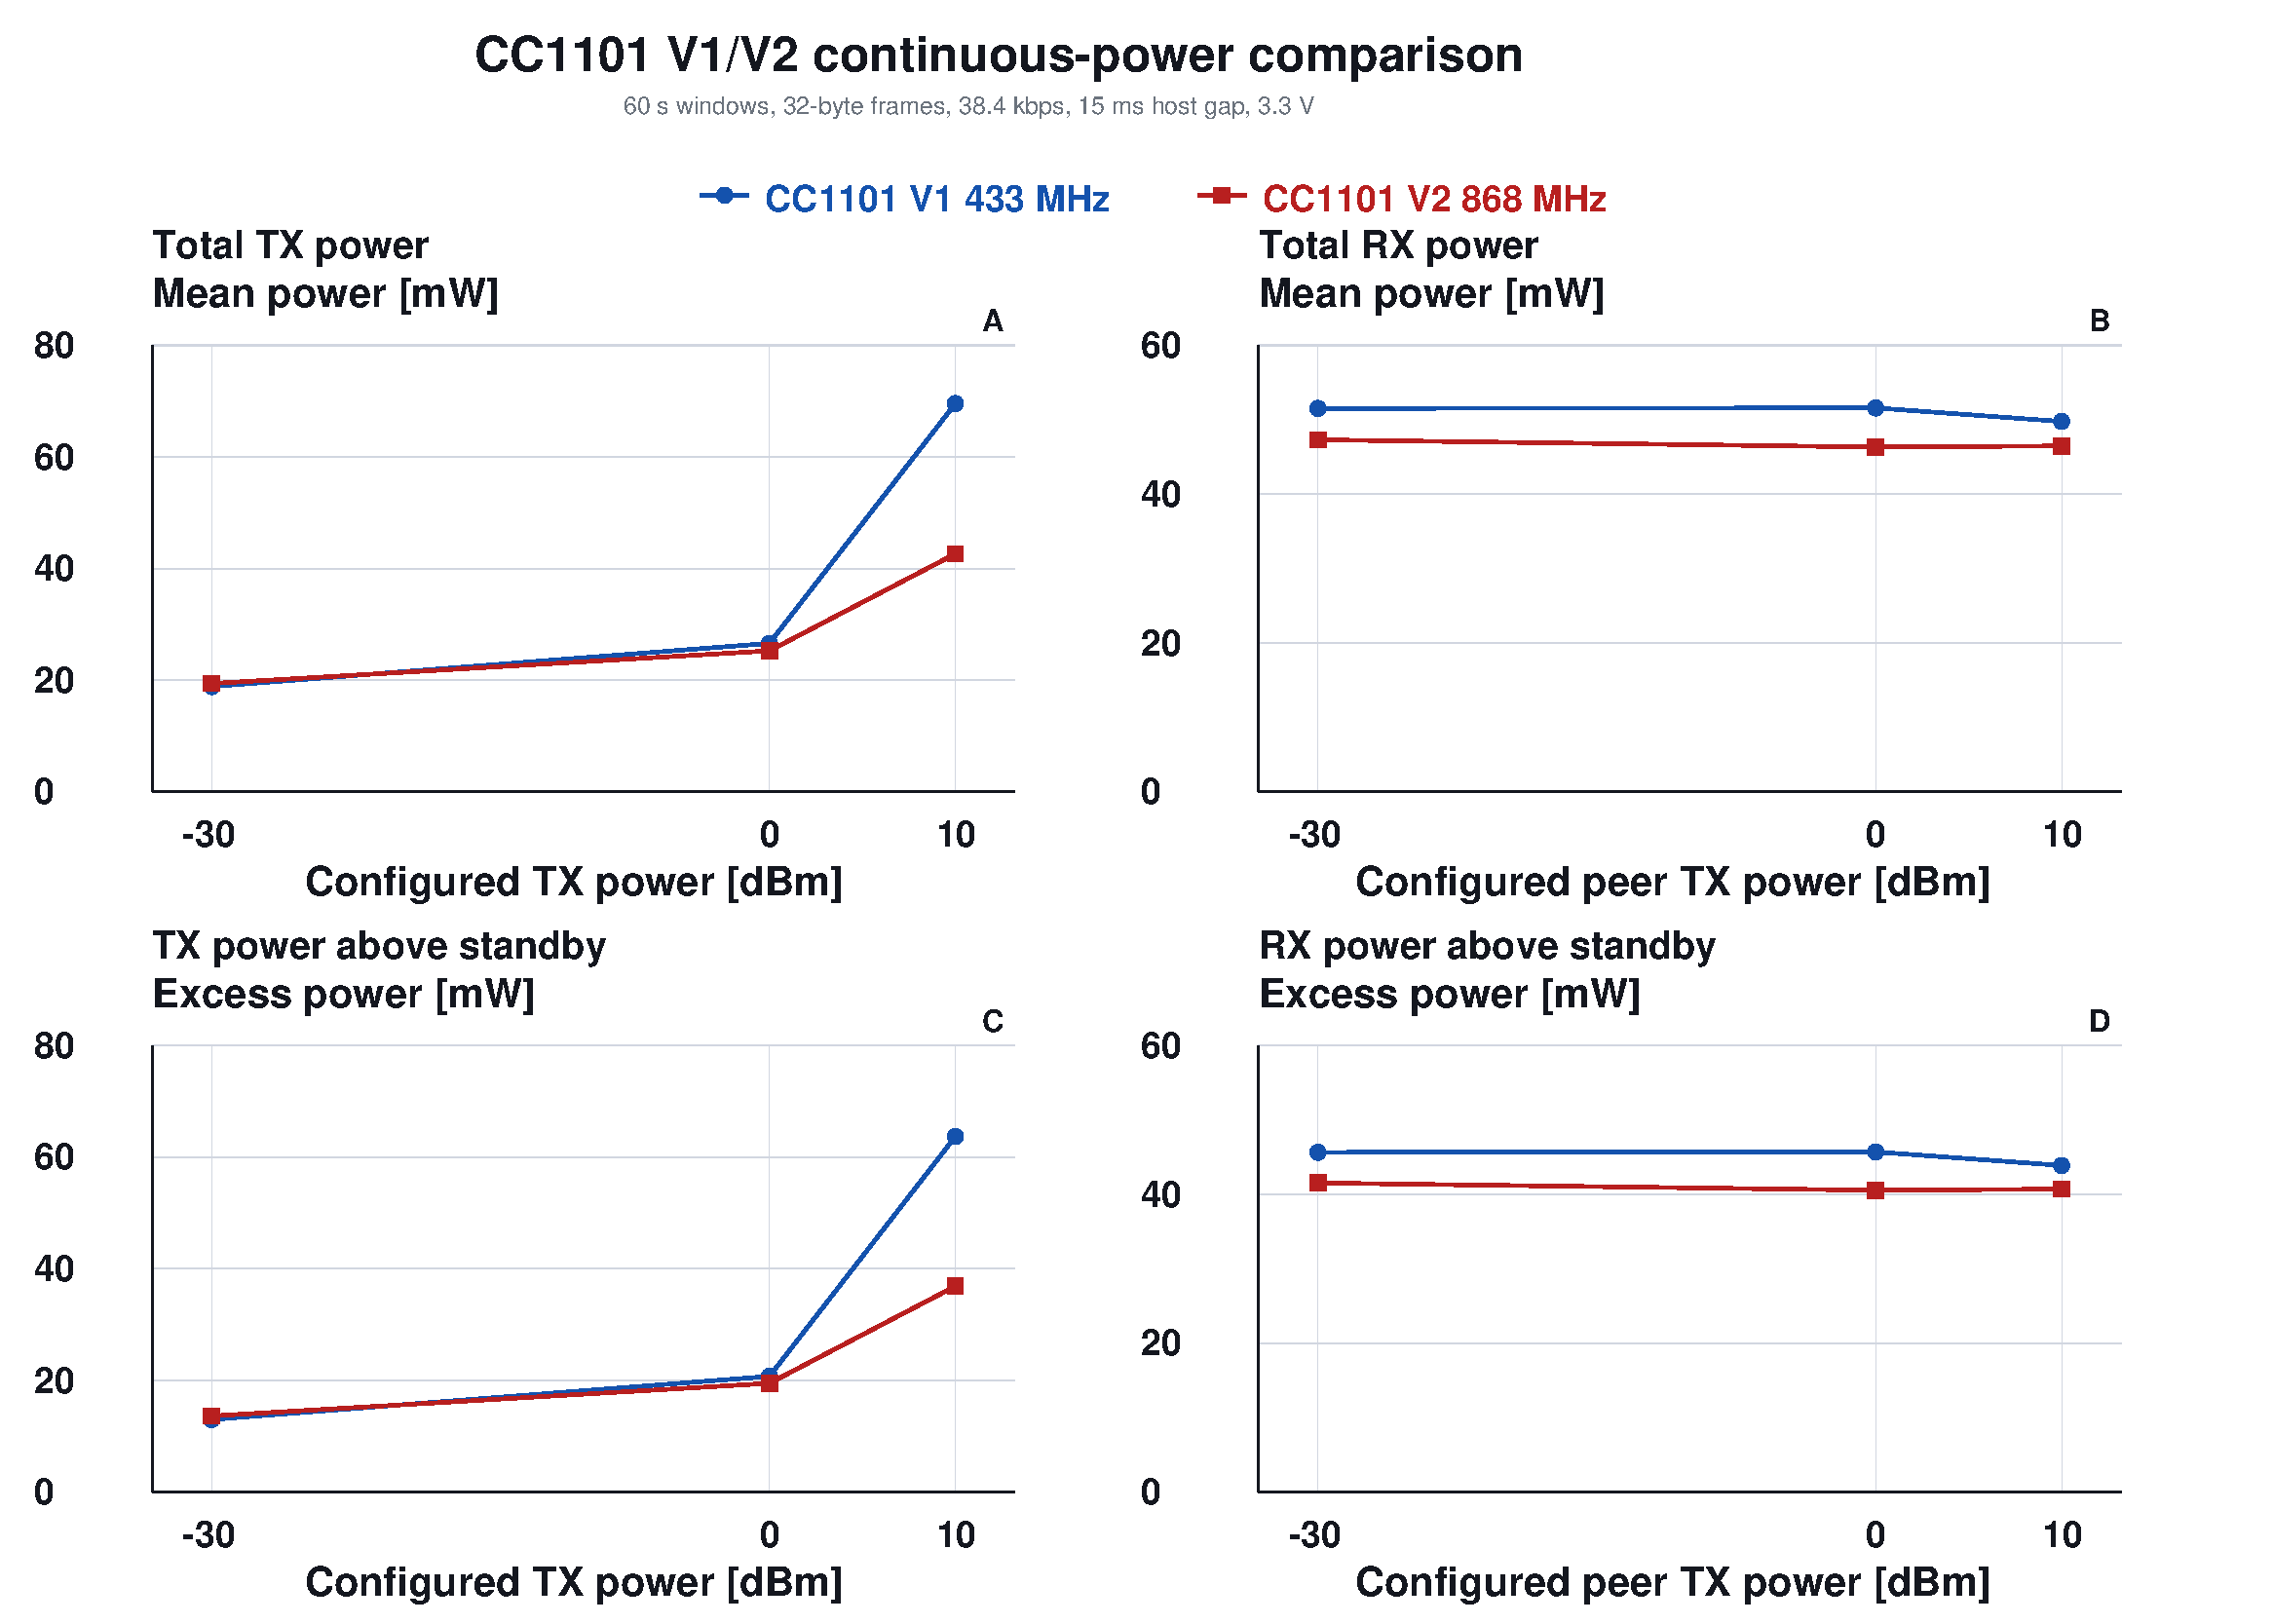
\includegraphics[width=\linewidth]{figures/cc1101_continuous_power_comparison.pdf}
  \caption{Controlled continuous-power comparison of the CC1101 V1 433-MHz and V2 868-MHz boards. Total and standby-subtracted values use the same 60-second, 32-byte, \SI{38.4}{kbps} workload. The configured power on RX is the peer transmitter setting.}
  \label{fig:cc1101-continuous}
\end{figure}

\begin{figure}[p]
  \centering
  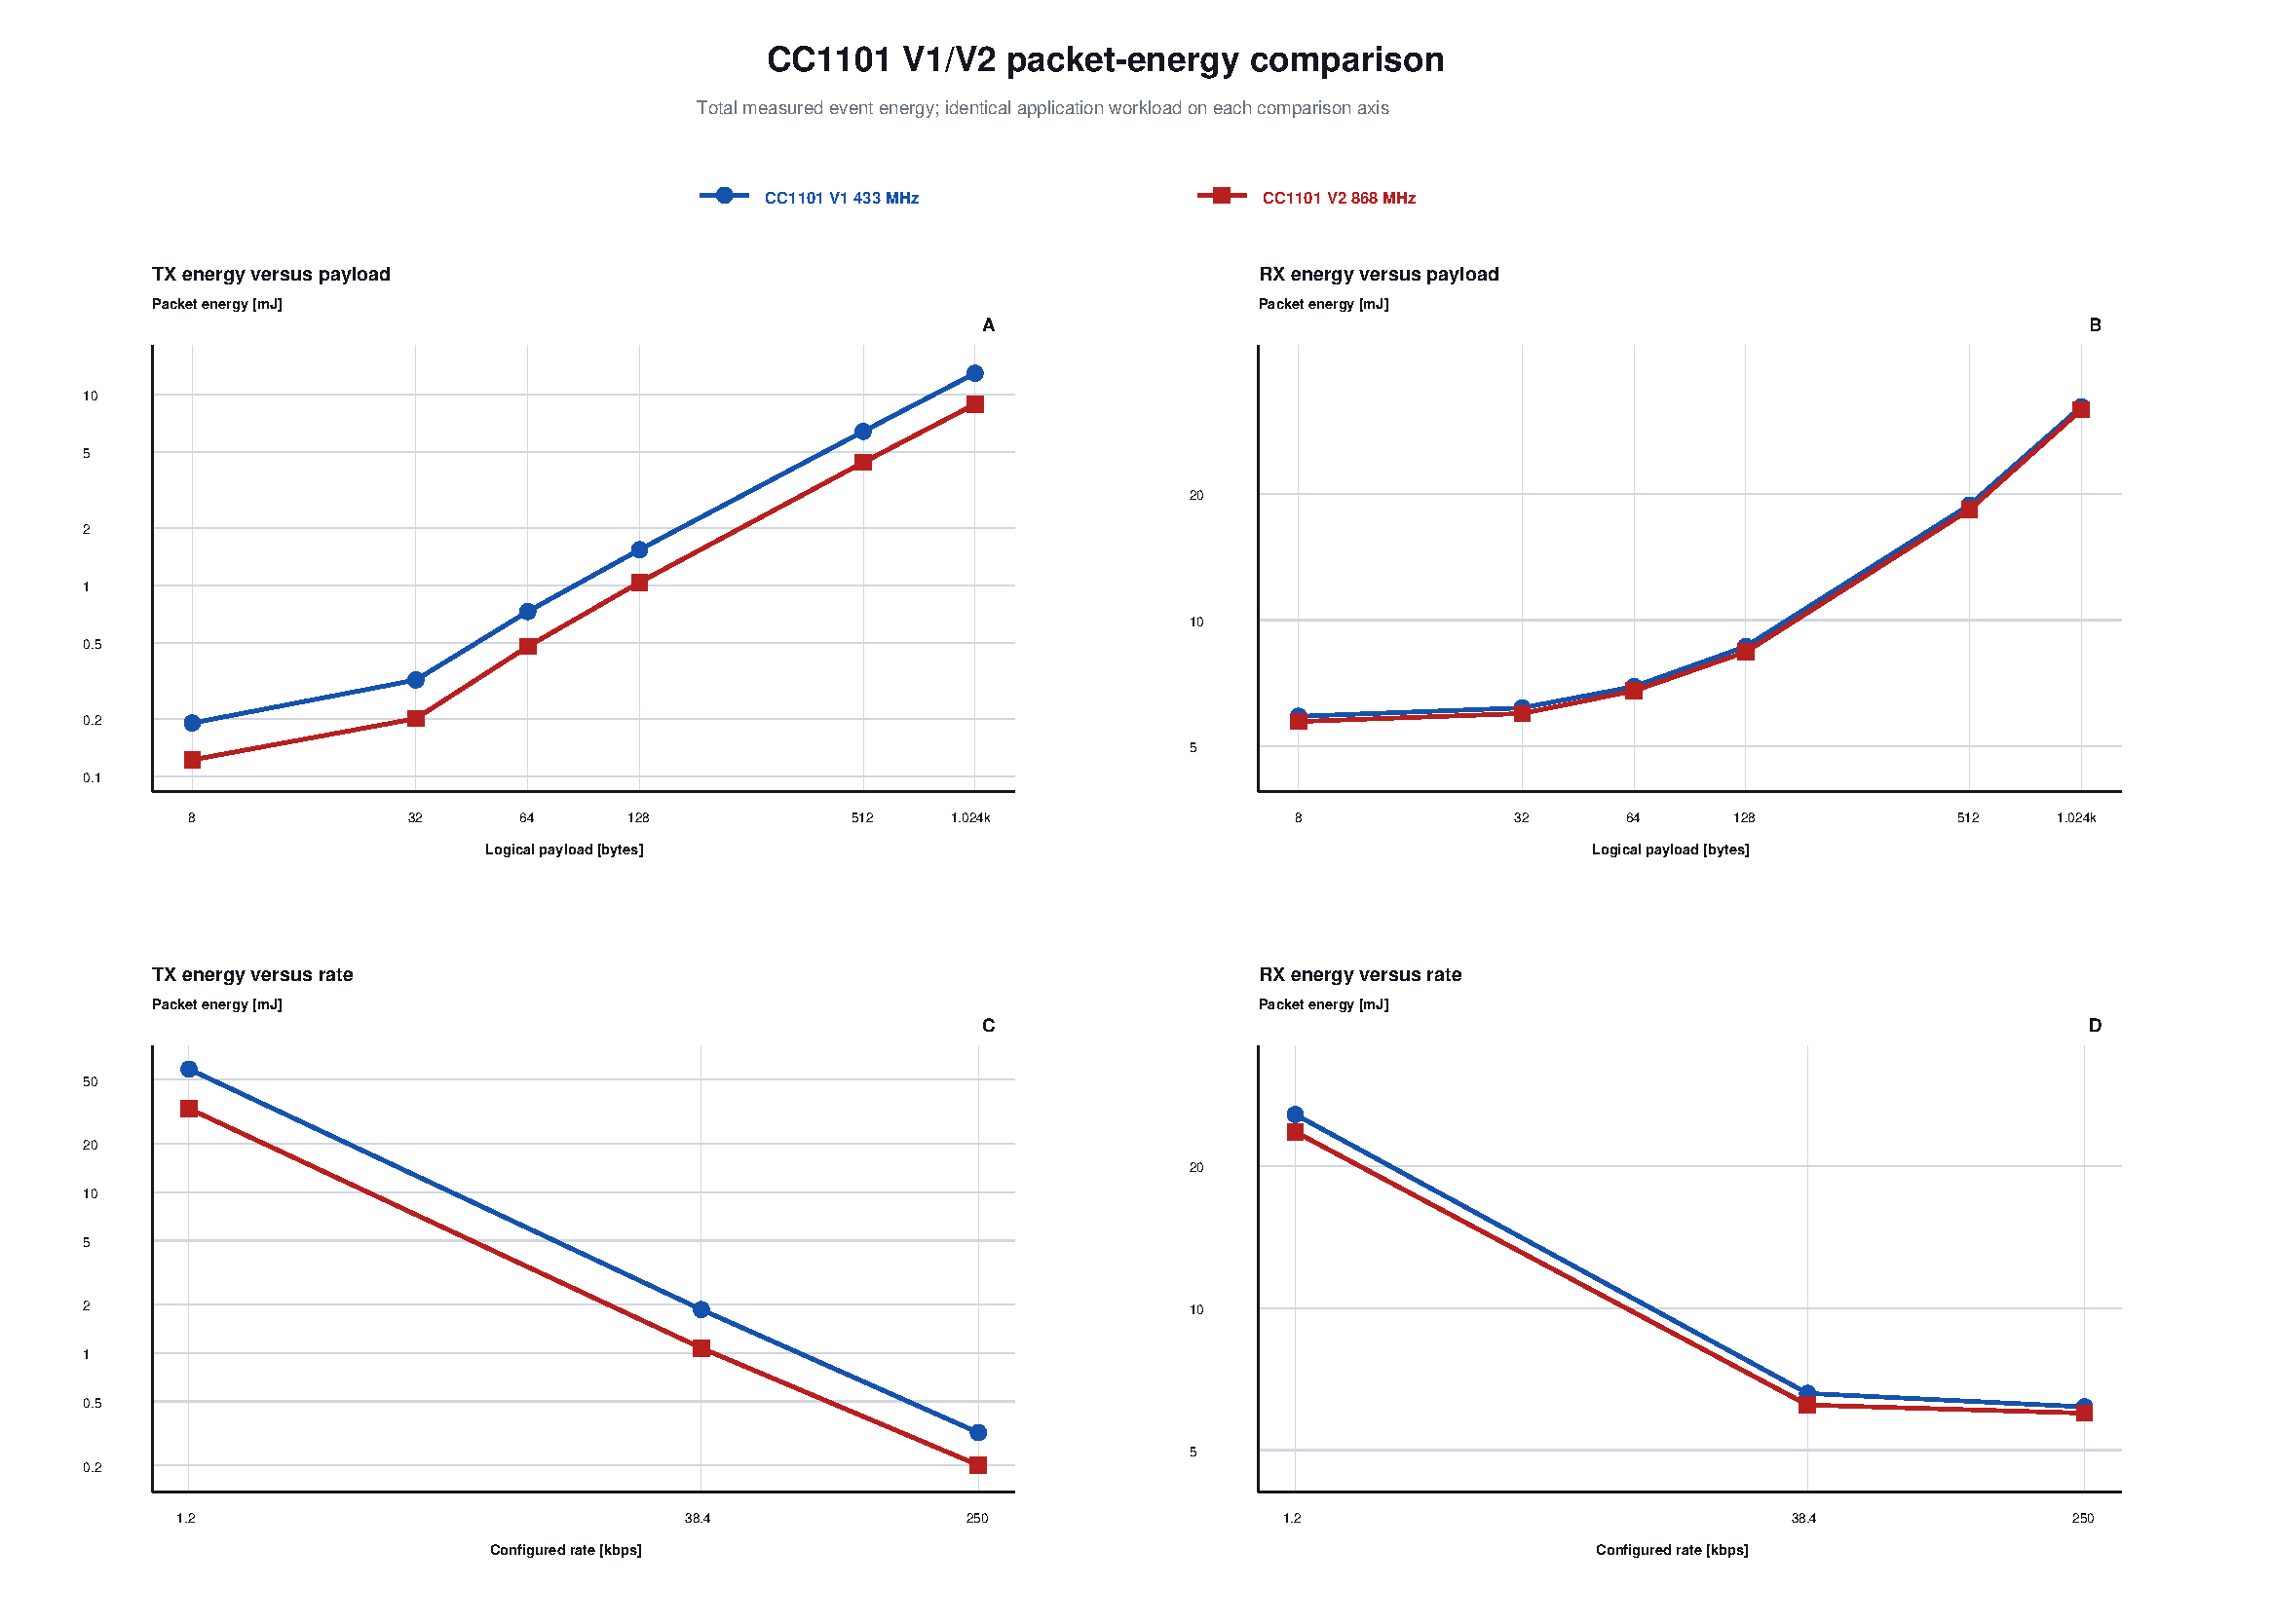
\includegraphics[width=\linewidth]{figures/cc1101_packet_comparison.pdf}
  \caption{CC1101 packet-energy scaling on common axes. Payload panels use \SI{250}{kbps} and +10 dBm; rate panels use a 32-byte payload and +10 dBm. Both axes are logarithmic.}
  \label{fig:cc1101-packet}
\end{figure}

Figures~\ref{fig:cc1101-continuous} and~\ref{fig:cc1101-packet} replace a single-point comparison with the complete common axes of the two campaigns. At 32 bytes, \SI{250}{kbps}, and +10 dBm, V2 uses \SI{0.201}{mJ} TX versus \SI{0.320}{mJ} for V1, a 37.2\% reduction. RX energy differs much less: \SI{5.990}{mJ} versus \SI{6.177}{mJ}. The pattern persists at 1024 bytes, where V2 uses \SI{8.874}{mJ} TX versus \SI{12.873}{mJ} for V1, while RX is \SI{31.695}{mJ} versus \SI{32.214}{mJ}. Rate scaling also shows the TX path as the dominant difference: at \SI{1.2}{kbps}, the 32-byte V2 event is \SI{33.11}{mJ}, compared with \SI{58.31}{mJ} for V1.

The continuous result is consistent with the packet result at high configured power. At +10 dBm, V2 averages \SI{42.65}{mW} TX versus \SI{69.58}{mW} for V1; after subtracting standby, the values are \SI{36.88}{mW} and \SI{63.70}{mW}. RX total power remains closer, between \SI{46.3}{mW} and \SI{47.3}{mW} for V2 versus \SI{49.8}{mW} to \SI{51.6}{mW} for V1. The -30 dBm V2 RX window delivered only 70.7\% of transmitted frames, compared with 99.95\% for V1, so that point is not equivalent useful work despite its lower mean power.

This is a controlled workload comparison, not a pure PCB-revision experiment: V1 operates at 433 MHz and V2 at 868 MHz. Frequency-dependent matching, configuration, board revision, and unit variation are confounded. The figures establish measured module-level behavior but do not assign its cause.

\subsection{Physical implementation effects}

\begin{figure}[htbp]
  \centering
  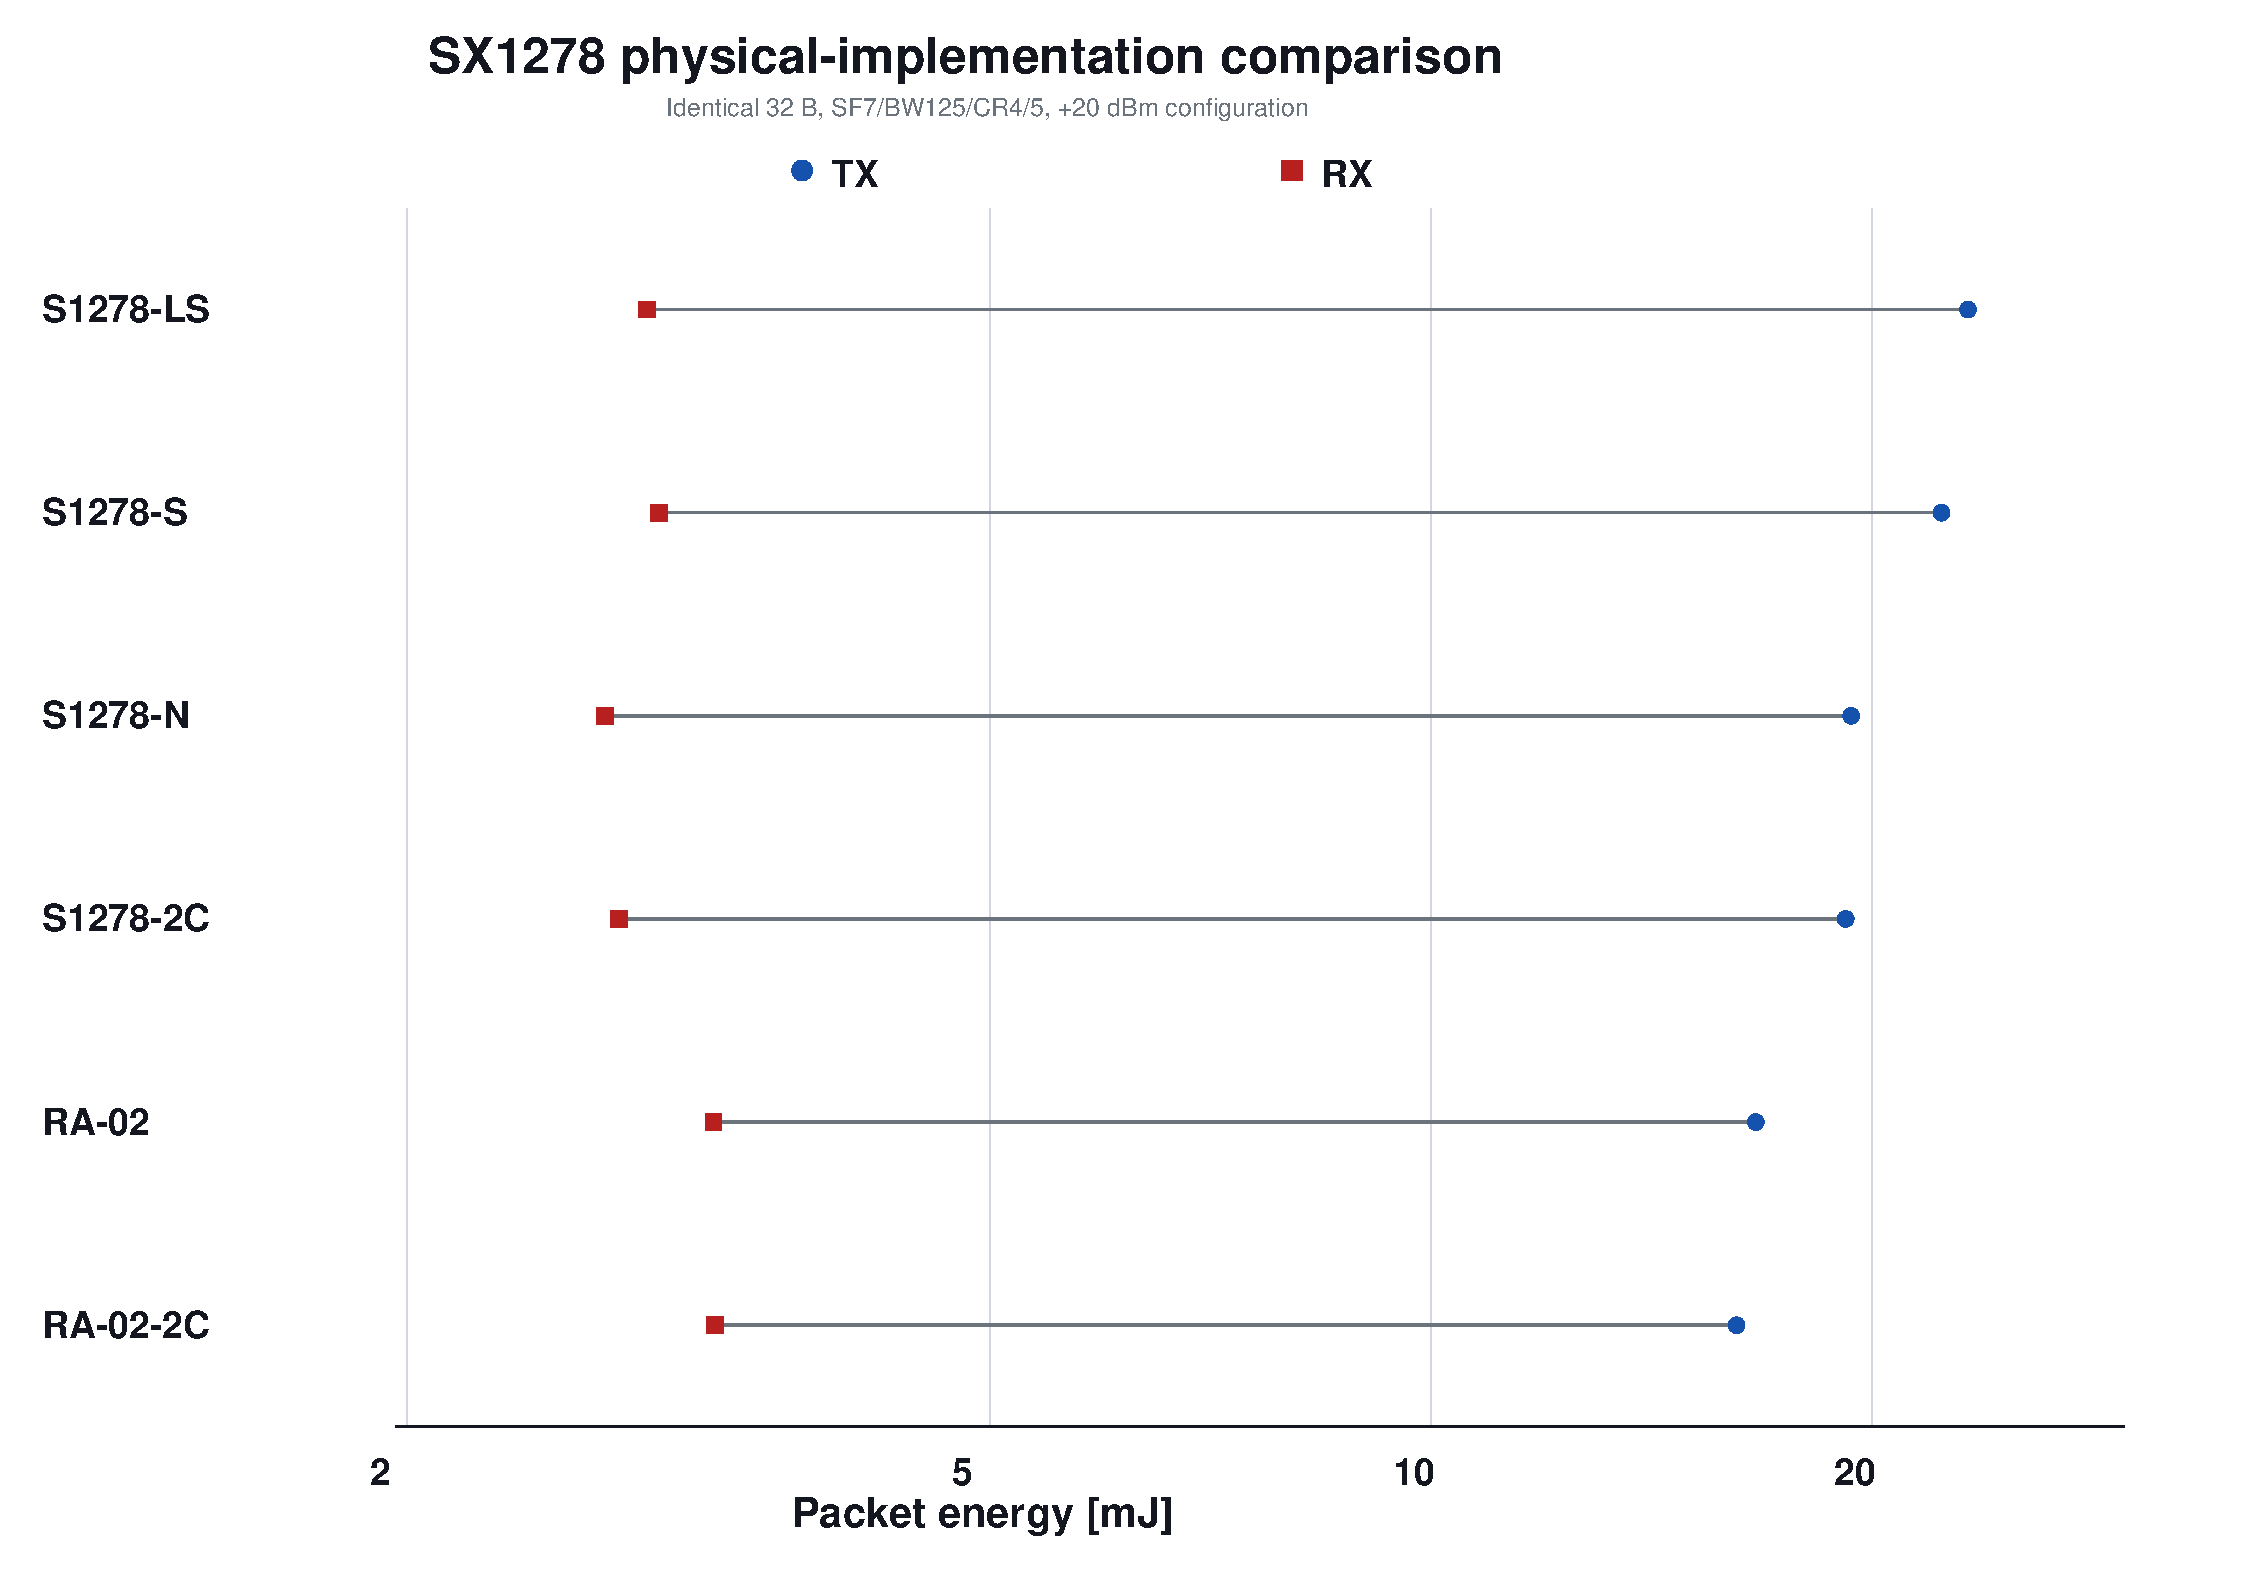
\includegraphics[width=\linewidth]{figures/sx1278_variant_comparison.pdf}
  \caption{Controlled SX1278 comparison at 32 bytes, SF7/BW125/CR4/5, and +20 dBm. The same radio settings do not produce identical board-level energy.}
  \label{fig:sx1278}
\end{figure}

The RA-02 with two added capacitors uses \SI{16.17}{mJ} versus \SI{16.67}{mJ} for the classic RA-02, a \SI{3.0}{\percent} reduction at this point. The custom naked board and its two-capacitor version differ by less than \SI{1}{\percent} in TX energy. Shielding and the level-shifter implementation are higher at \SI{22.32}{mJ} and \SI{23.27}{mJ}, respectively, compared with \SI{19.36}{mJ} for the naked board. These are module-boundary observations; the experiment does not isolate regulator quiescent current, RF matching loss, logic translation, and oscillator behavior sufficiently to assign a single cause.

\begin{figure}[p]
  \centering
  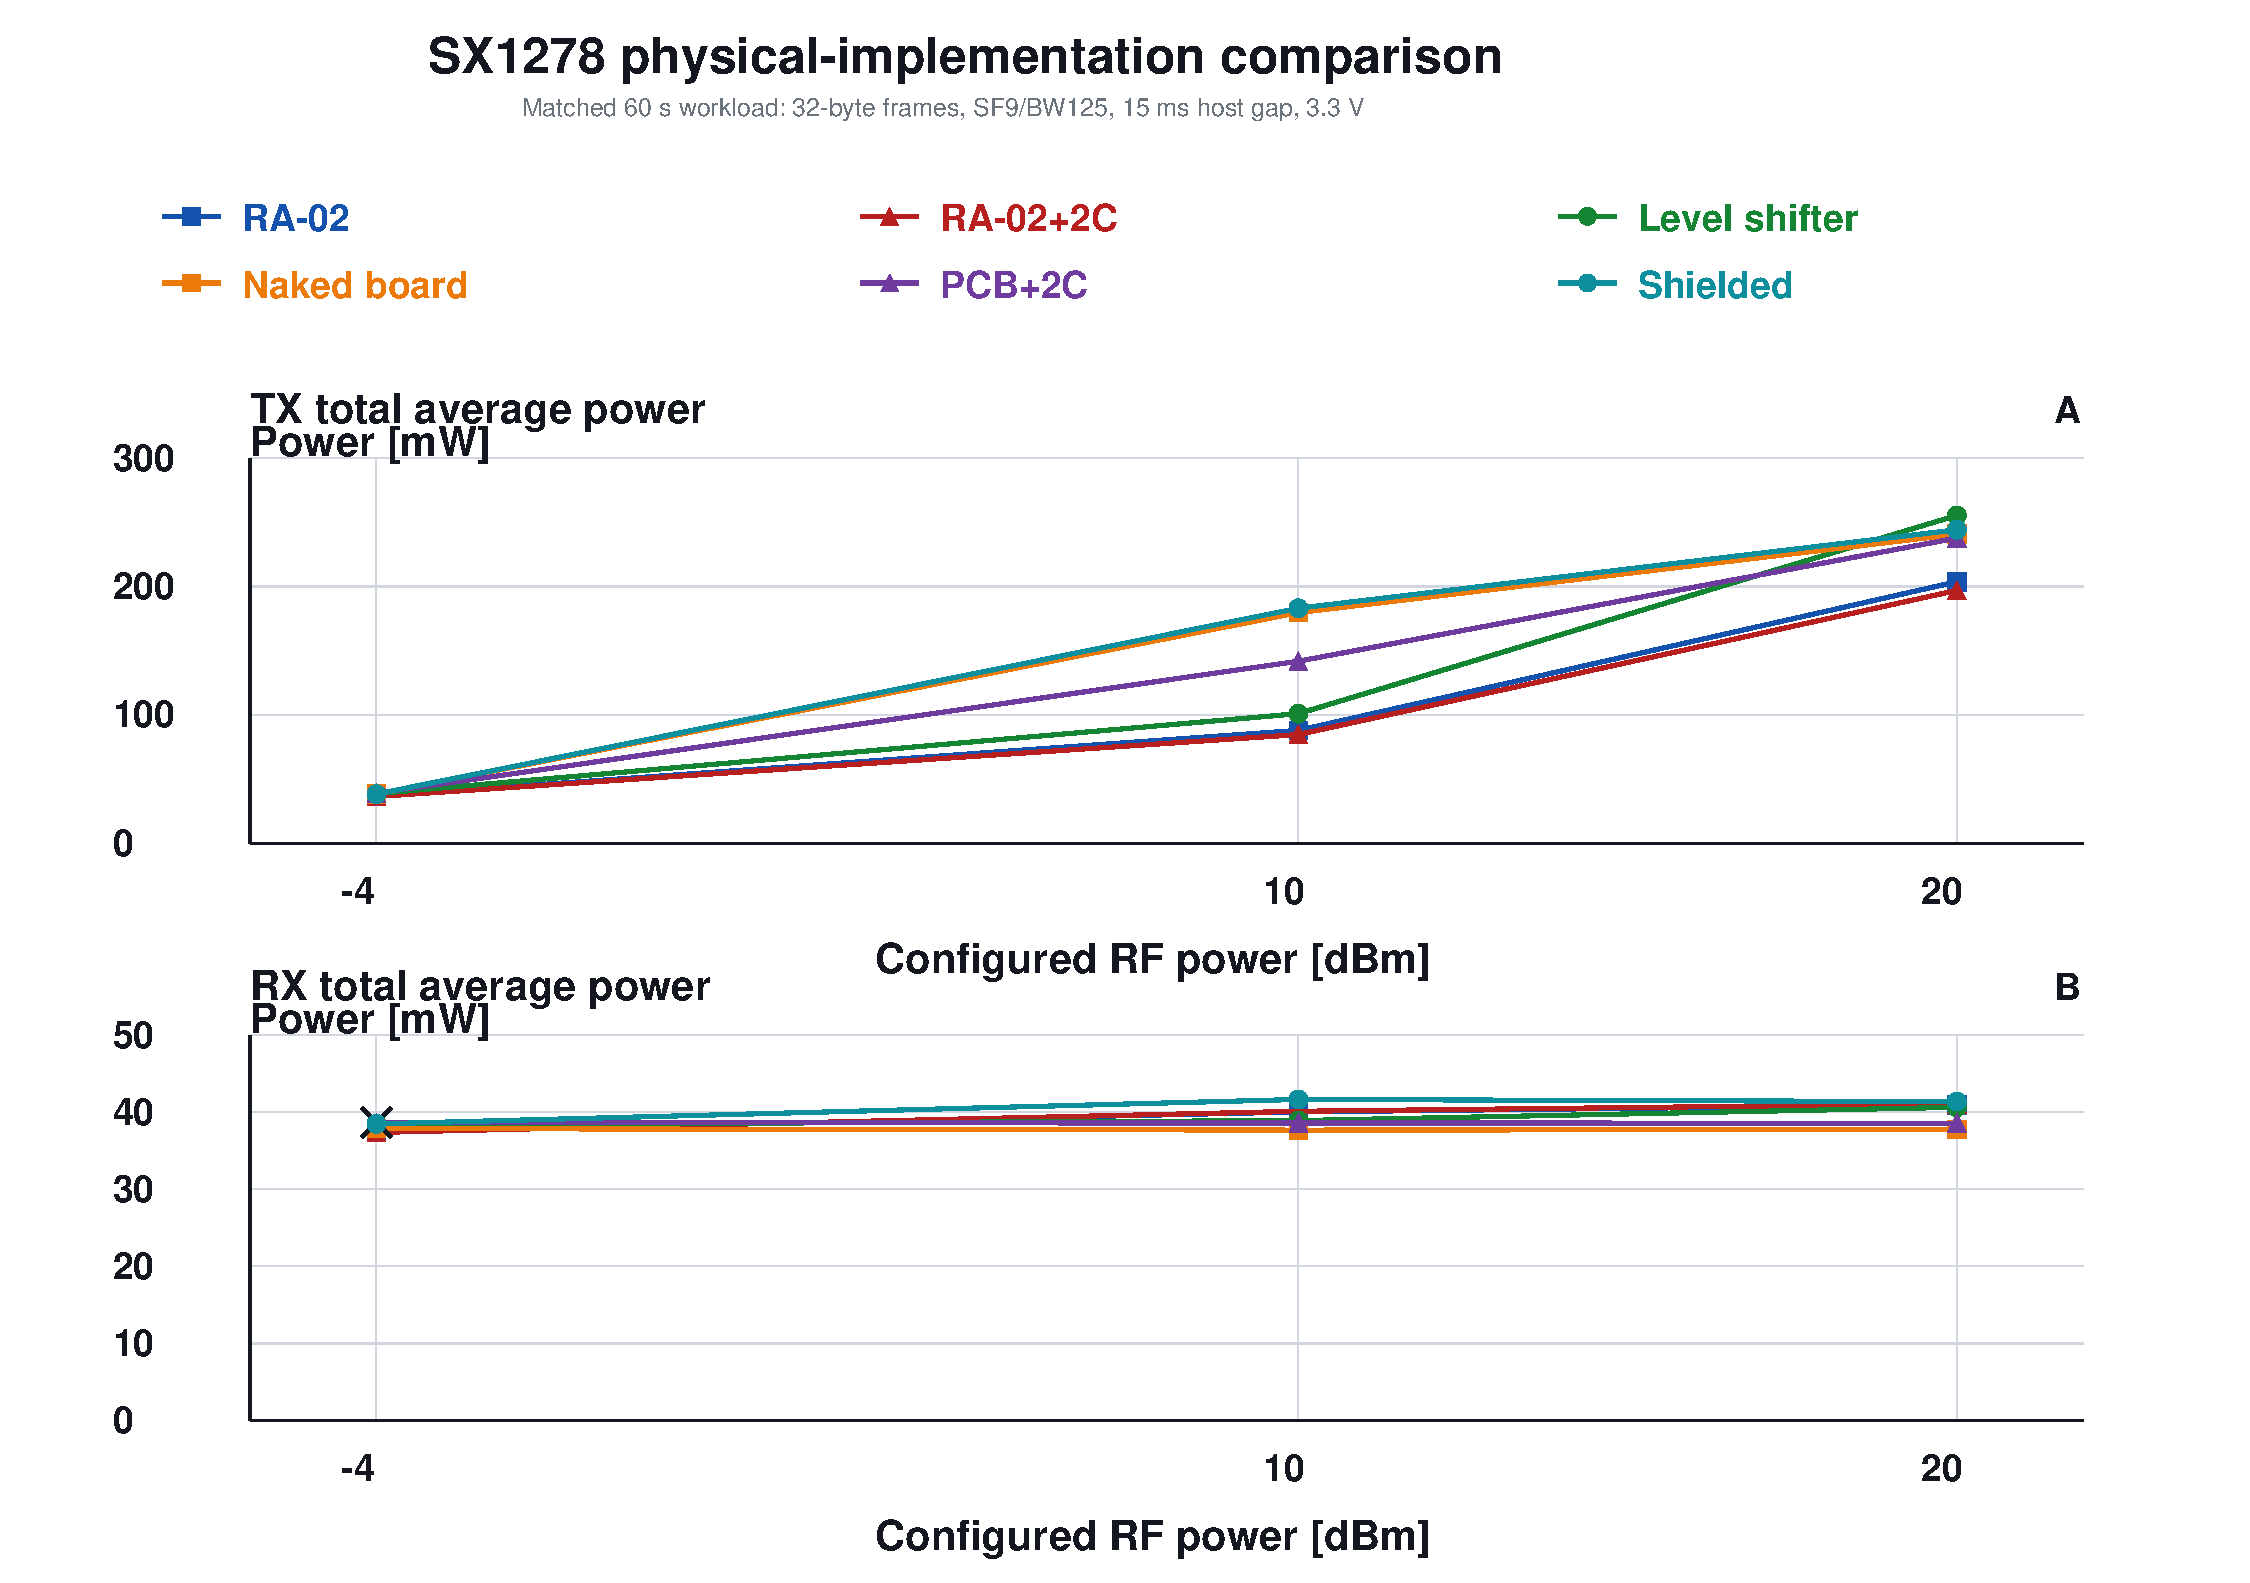
\includegraphics[width=\linewidth]{figures/sx1278_continuous_power_comparison.pdf}
  \caption{Matched continuous total-power comparison for all six SX1278 implementations from Figure~\ref{fig:sx1278}. The TX and RX panels use independent vertical scales so that board-level differences remain visible.}
  \label{fig:sx1278-continuous}
\end{figure}

\begin{figure}[p]
  \ContinuedFloat
  \centering
  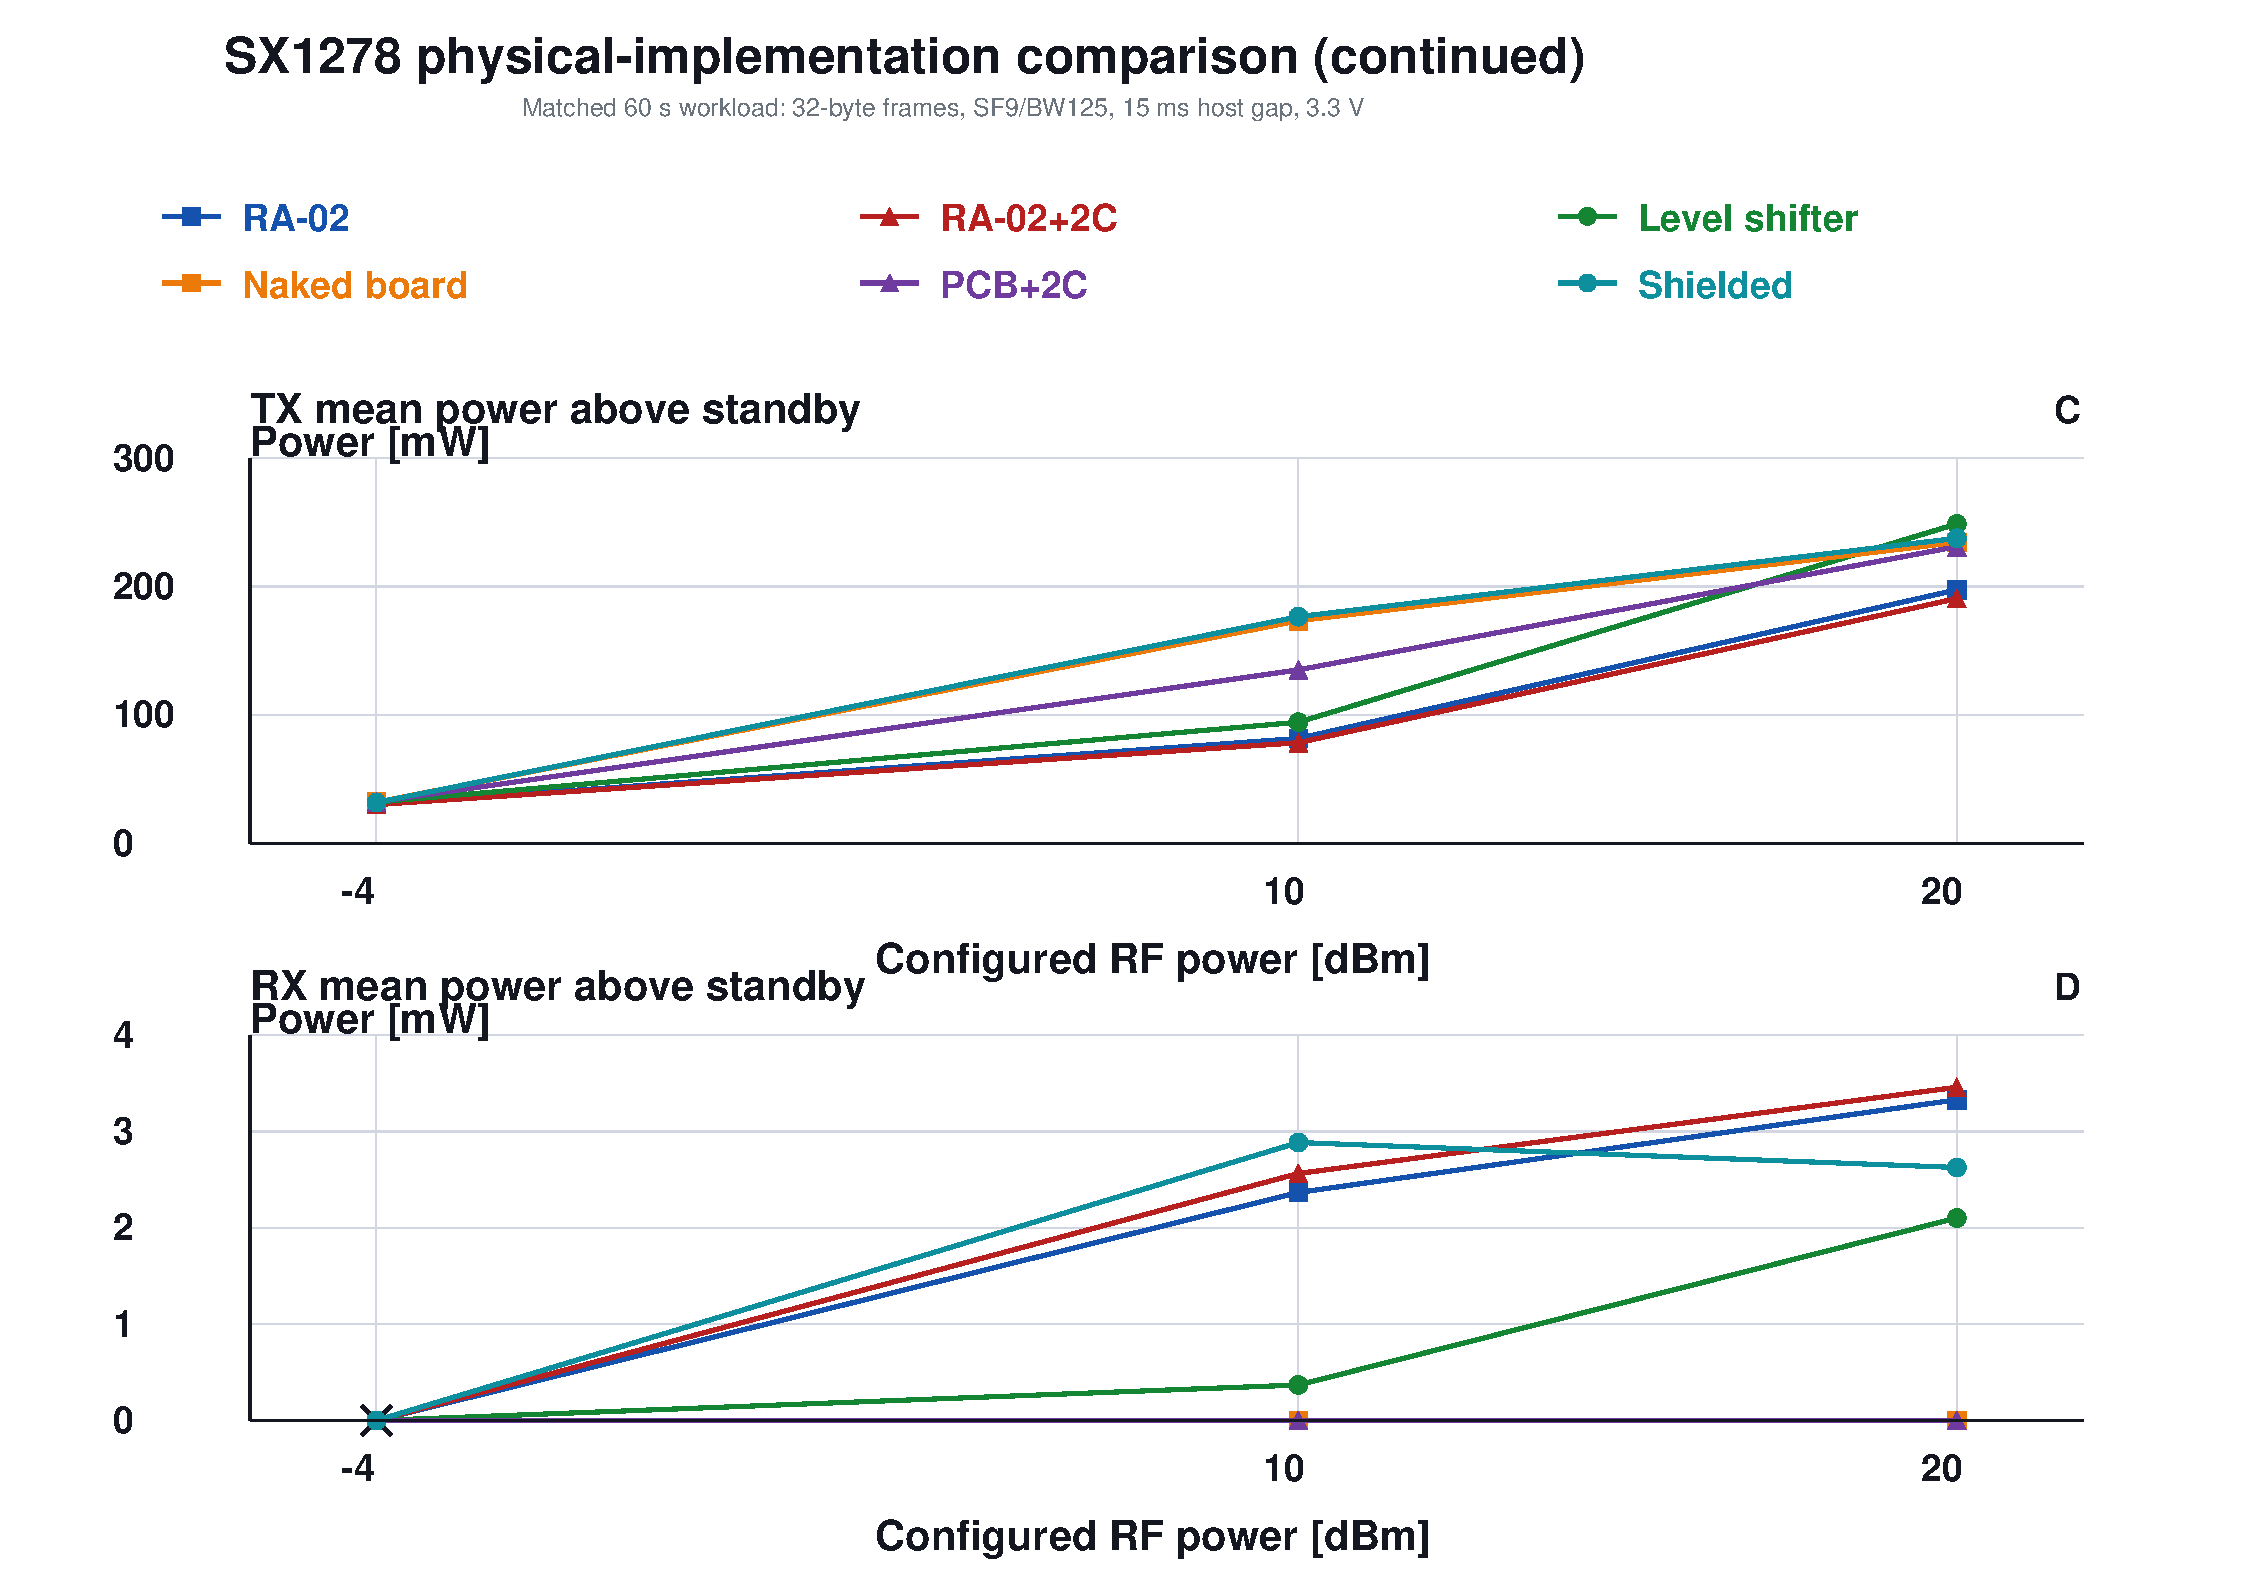
\includegraphics[width=\linewidth]{figures/sx1278_continuous_power_comparison_continued.pdf}
  \caption[]{Matched continuous-power comparison for all six SX1278 implementations (continued): standby-subtracted TX and RX power. A black cross marks the S1278-2C RX window at $-4$ dBm, whose power trace is valid but whose receiver-delivery telemetry is missing.}
\end{figure}

Figure~\ref{fig:sx1278-continuous} extends the packet-only comparison to every available 60-second SF9/BW125 window. At +20 dBm, total TX power ranges from \SI{196.94}{mW} for RA-02+2C to \SI{255.33}{mW} for the level-shifter board, while total RX power occupies a narrower \SI{37.75--41.37}{mW} interval. The S1278-2C RX point at $-4$ dBm is retained only as a power observation: zero received frames prevent it from supporting a useful-delivery conclusion.

Within this six-board view, the continuous TX reduction from adding two capacitors to RA-02 is \SI{0.36}{\percent} at $-4$ dBm, \SI{3.71}{\percent} at +10 dBm, and \SI{3.31}{\percent} at +20 dBm. At +20 dBm, this corresponds to \SI{196.94}{mW} versus \SI{203.69}{mW}. RX total power differs by at most \SI{0.3}{\percent}, so the added capacitors do not produce a meaningful receive-power advantage in this workload. The repeated few-percent TX effect at the two higher settings is measurable, but the experiment does not establish whether it comes from supply impedance, PA behavior, or RF matching.

\begin{figure}[htbp]
  \centering
  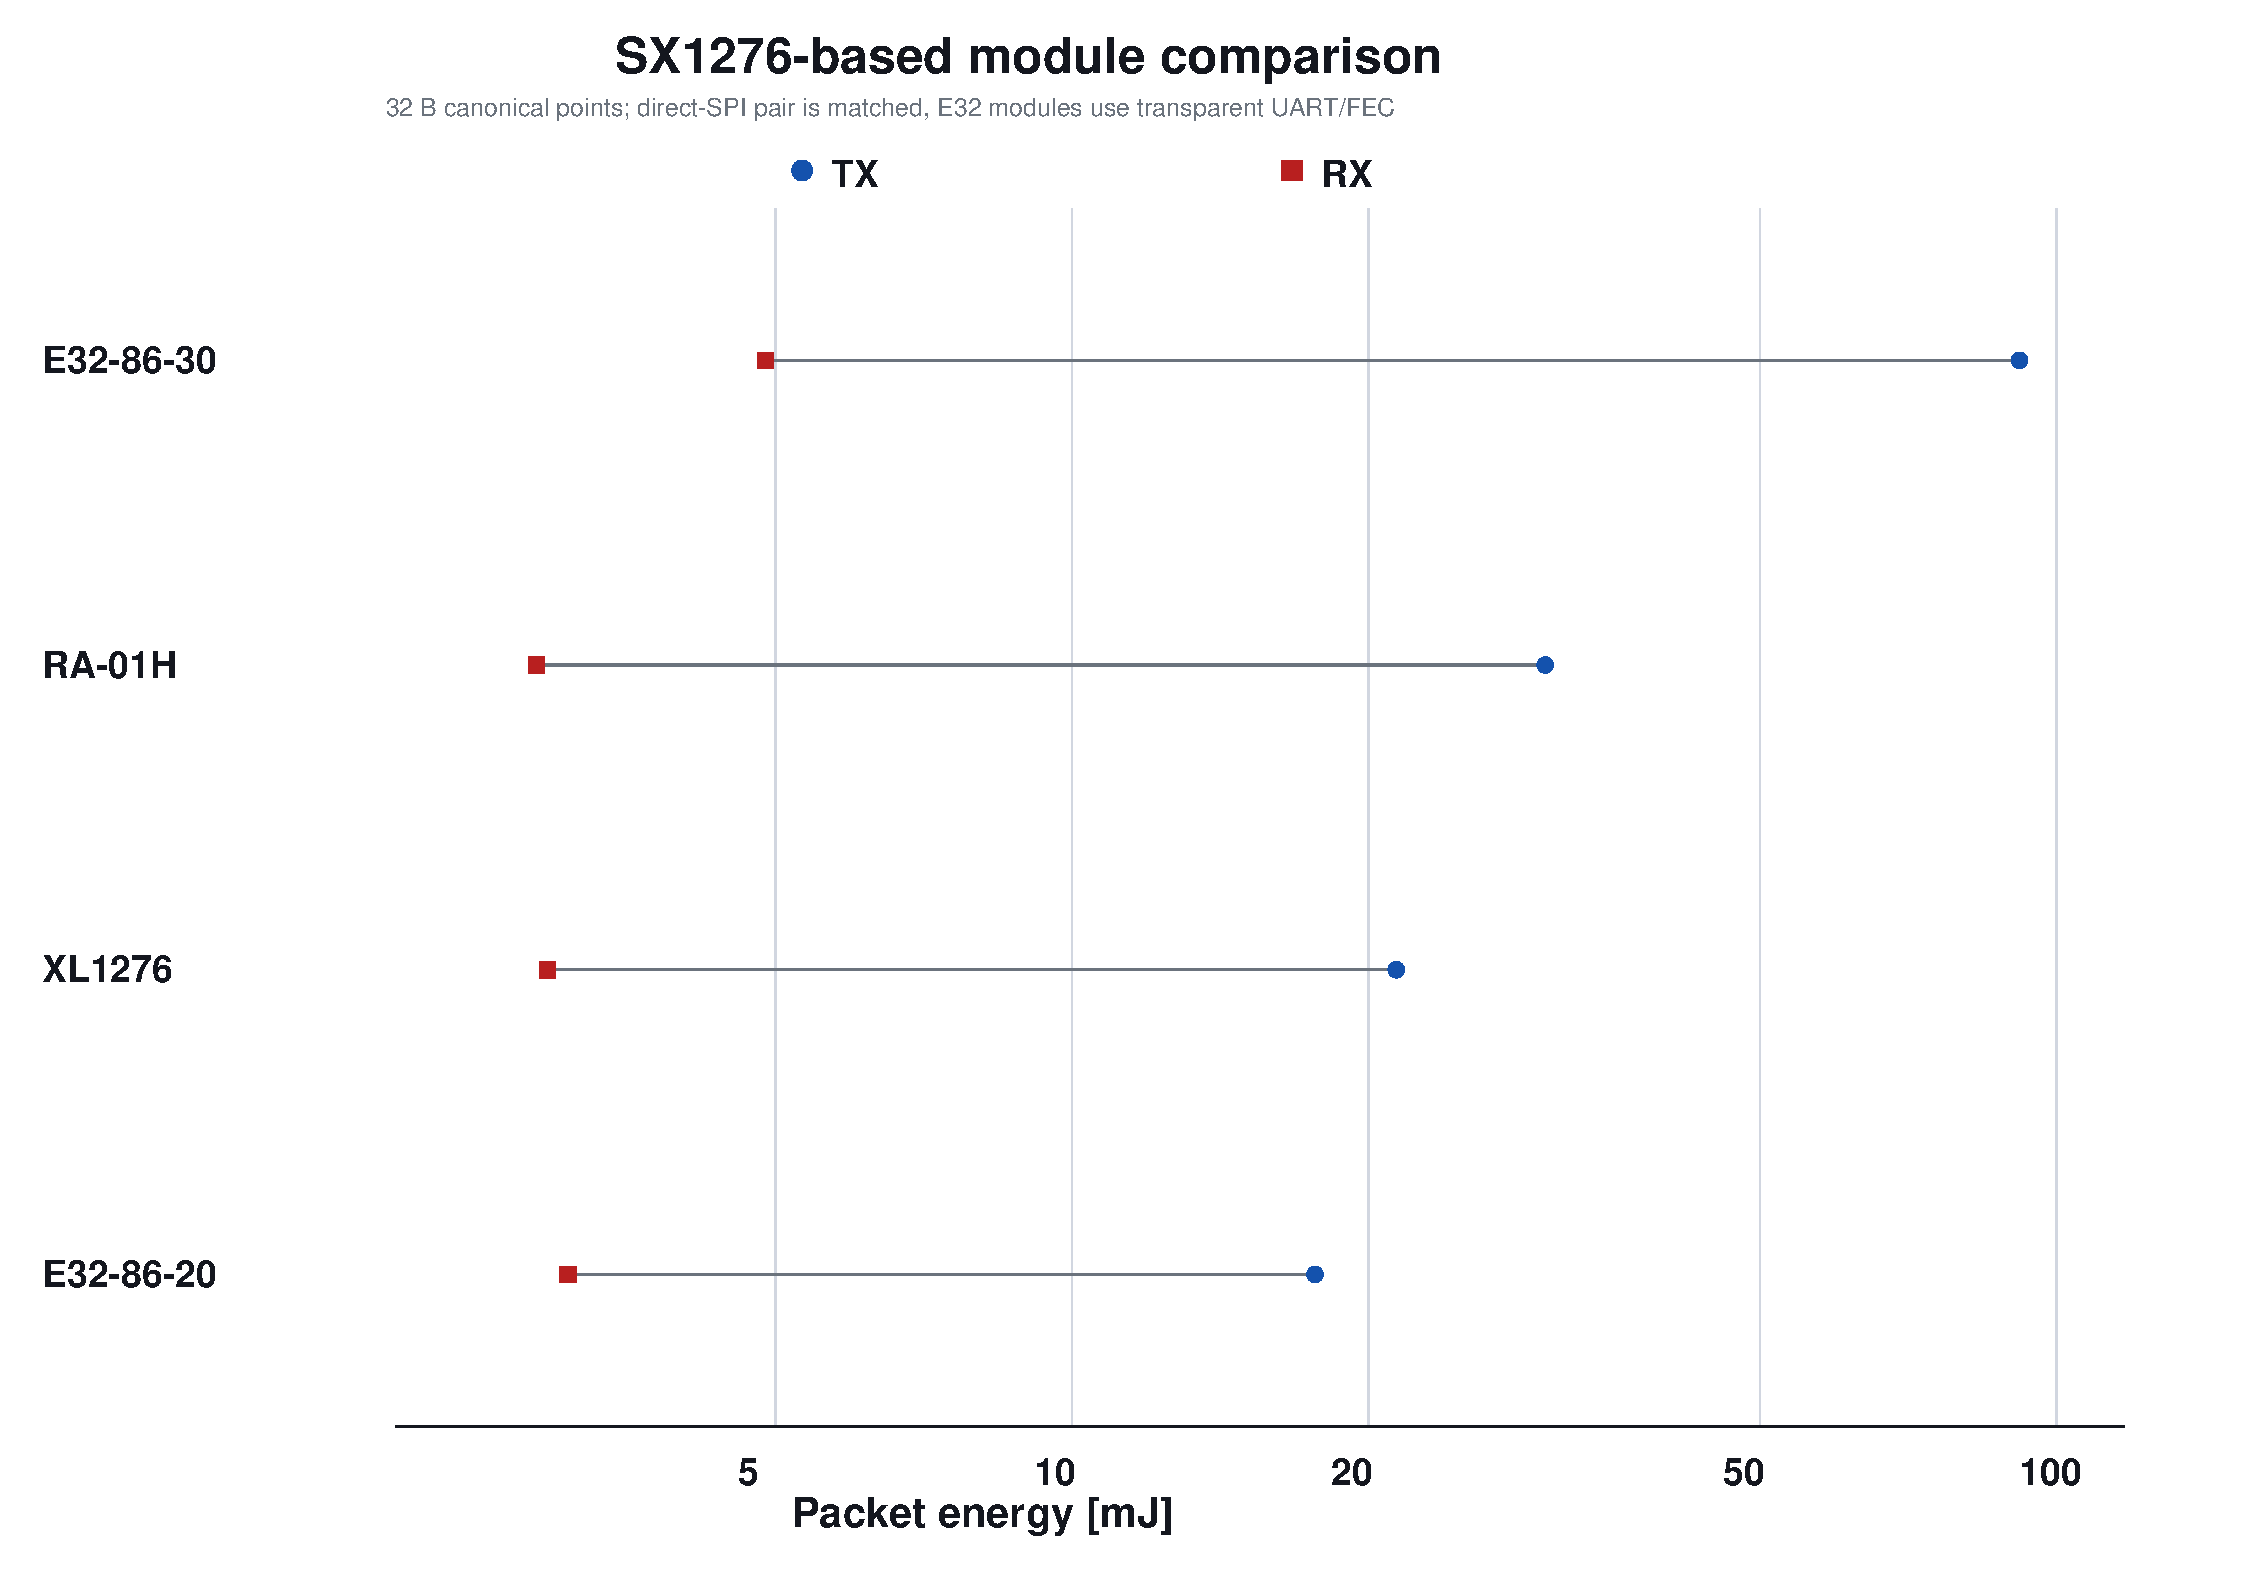
\includegraphics[width=\linewidth]{figures/sx1276_variant_comparison.pdf}
  \caption{All four measured SX1276-based modules at their canonical 32-byte points. RA-01H and XL1276-D01 use direct SPI, SF7/BW125/CR4/5, and +20 dBm. E32-868T20D and E32-868T30D use transparent UART/FEC at \SI{19.2}{kbps} and +20 dBm or +30 dBm, respectively. The latter includes an external PA, so the four points are a complete system-level inventory, not a single controlled operating condition.}
  \label{fig:sx1276}
\end{figure}

\begin{figure}[p]
  \centering
  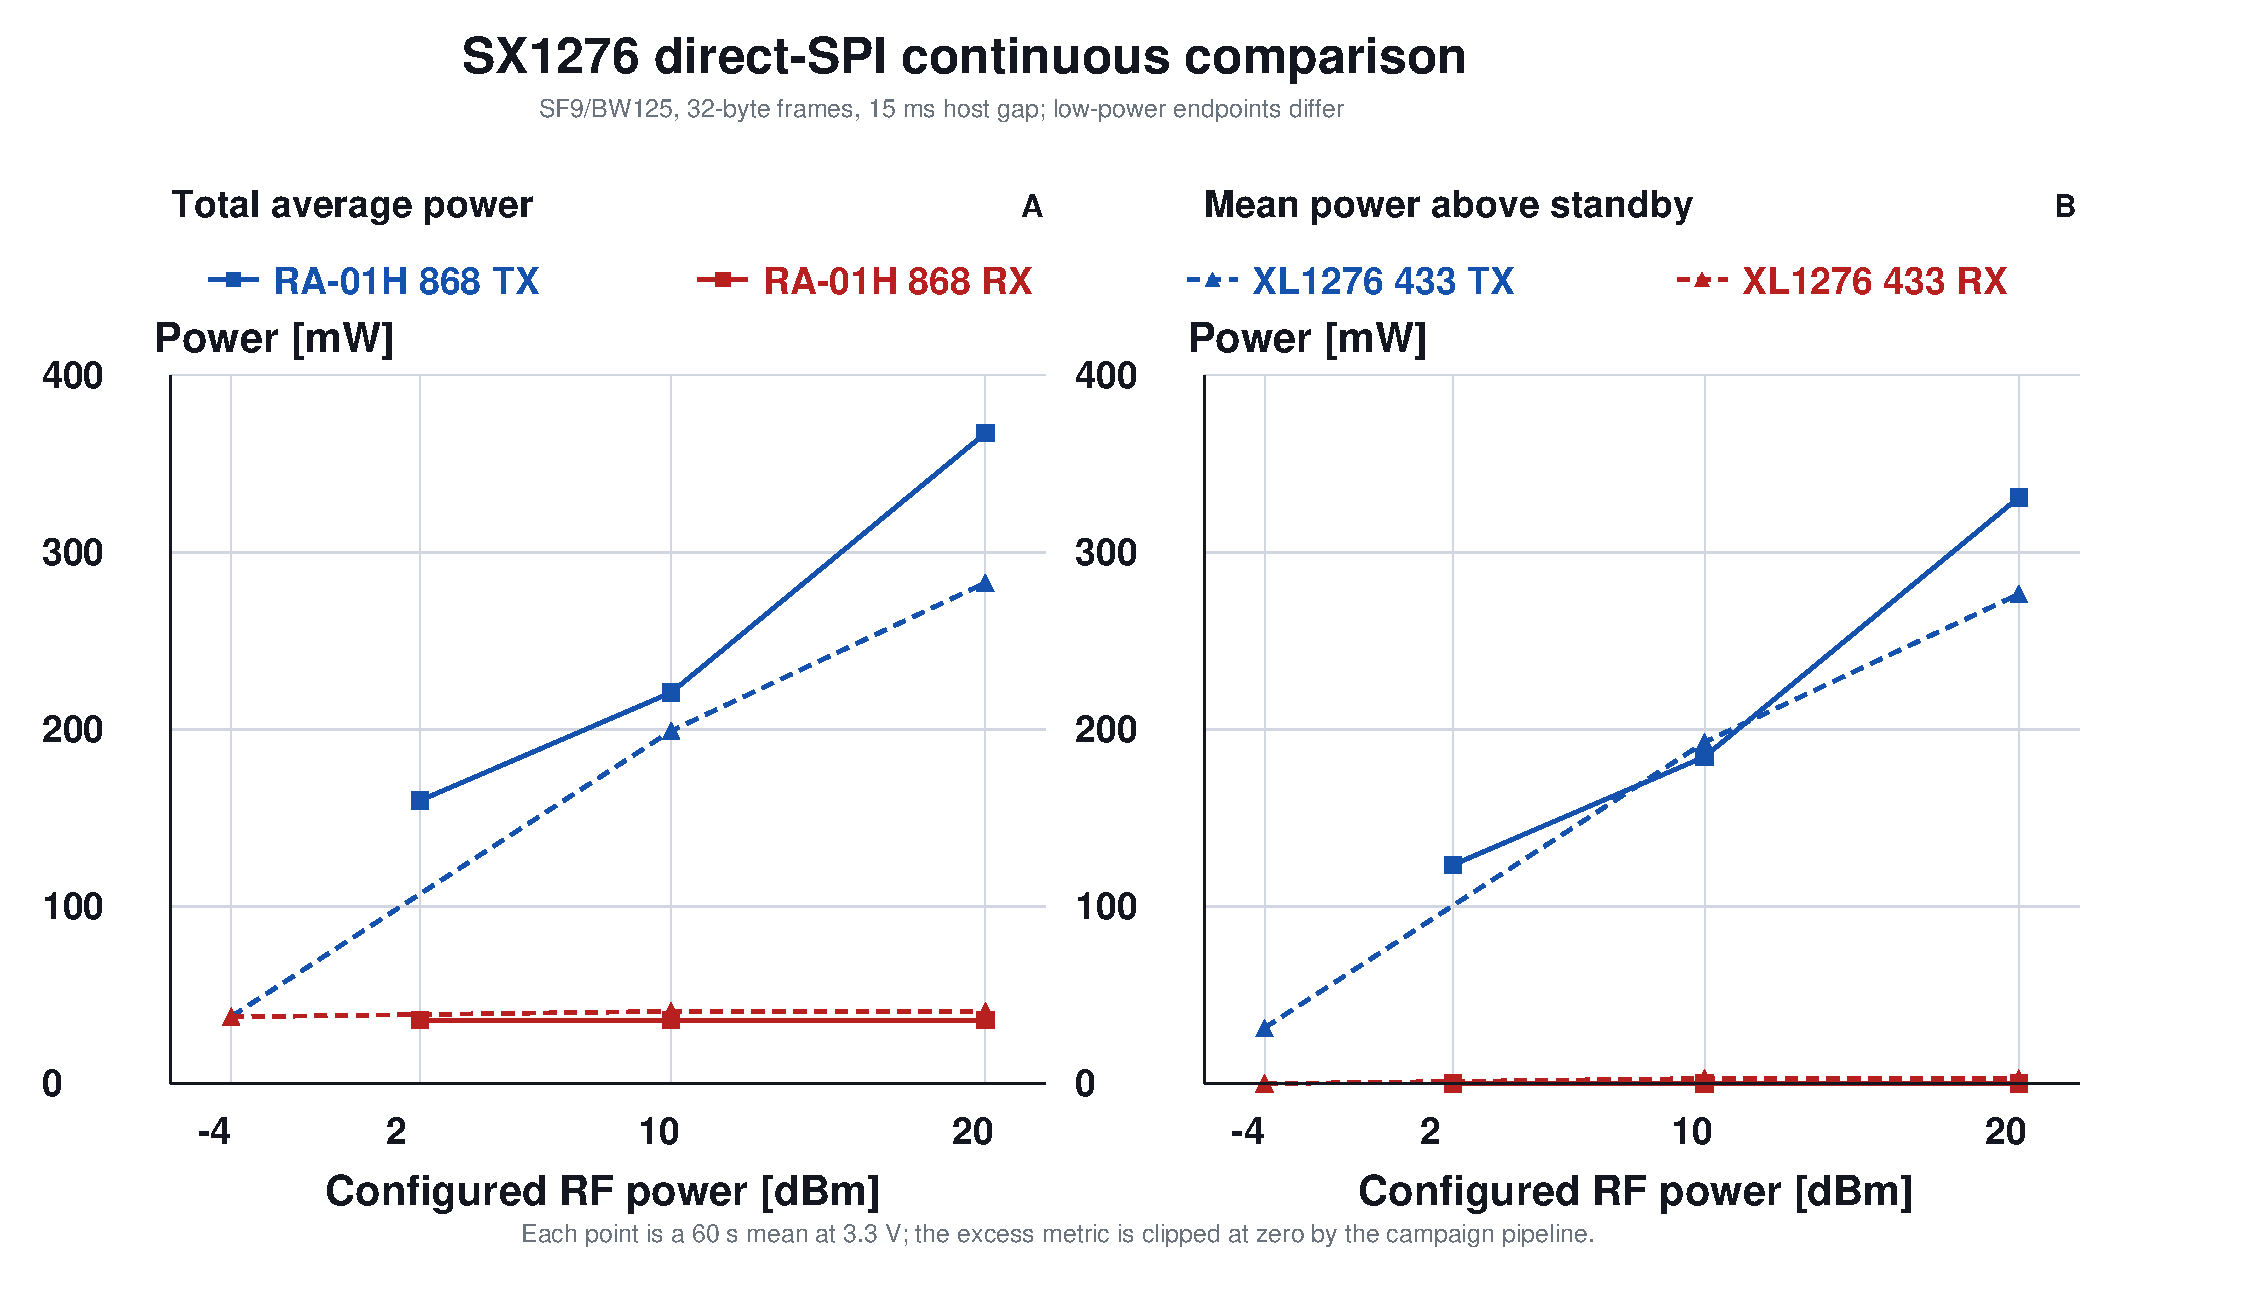
\includegraphics[width=0.96\linewidth]{figures/sx1276_continuous_power_comparison.pdf}
  \caption{Controlled continuous-power comparison of the direct-SPI SX1276 subset, RA-01H and XL1276-D01, at SF9/BW125. Both include +10 and +20 dBm; the low endpoint is +2 dBm for RA-01H and $-4$ dBm for XL1276-D01.}
  \label{fig:sx1276-continuous}
\end{figure}

The repository audit identifies four measured SX1276-based implementations: RA-01H, XL1276-D01, E32-868T20D, and E32-868T30D. Figure~\ref{fig:sx1276} retains all four. At their canonical points, packet TX energy is \SI{17.66}{mJ}, \SI{21.35}{mJ}, \SI{30.24}{mJ}, and \SI{91.65}{mJ} for E32-868T20D, XL1276-D01, RA-01H, and E32-868T30D, respectively. RX spans a much narrower \SI{2.860--4.884}{mJ}. These values are useful module-level operating points, but the E32 transparent-UART framing, higher nominal rate, and the T30D external PA prevent a controlled four-way PHY comparison.

Within the matched direct-SPI subset, XL1276-D01 uses \SI{21.35}{mJ} TX versus \SI{30.24}{mJ} for RA-01H, a \SI{29.4}{\percent} reduction, while RX is \SI{2.934}{mJ} versus \SI{2.860}{mJ}. In continuous operation at +20 dBm, XL1276-D01 averages \SI{282.87}{mW} TX versus \SI{367.36}{mW} for RA-01H; RX reverses the ordering at \SI{40.78}{mW} versus \SI{35.87}{mW}. These are same-chip, same-LoRa-setting observations, but not a pure PCB comparison because the RF bands, matching networks, and individual units differ.

The same audit found no additional measured SX1276 modules: RA-01 and the 433-MHz E32 units are SX1278 implementations, while RFM9x and inAir9 occur only as KiCad library footprints without campaigns. E28 and E280 both use SX1280 but expose direct-SPI LoRa and vendor transparent-UART PHYs, respectively. Their results remain valid system-level measurements, but their framing and control paths prevent attribution of a difference to the radio board alone.

The newer RA-01SH/SX1262 is notable: at its canonical +22 dBm point it uses \SI{18.03}{mJ} TX and \SI{1.185}{mJ} RX, versus \SI{30.24}{mJ} and \SI{2.860}{mJ} for the RA-01H/SX1276 at +20 dBm. Its matched continuous RX power is \SI{14.76}{mW} versus \SI{35.87}{mW}. The measured reduction is consistent with, but does not independently prove, the SX1262's newer low-power receiver and DC--DC architecture.

\begin{figure}[htbp]
  \centering
  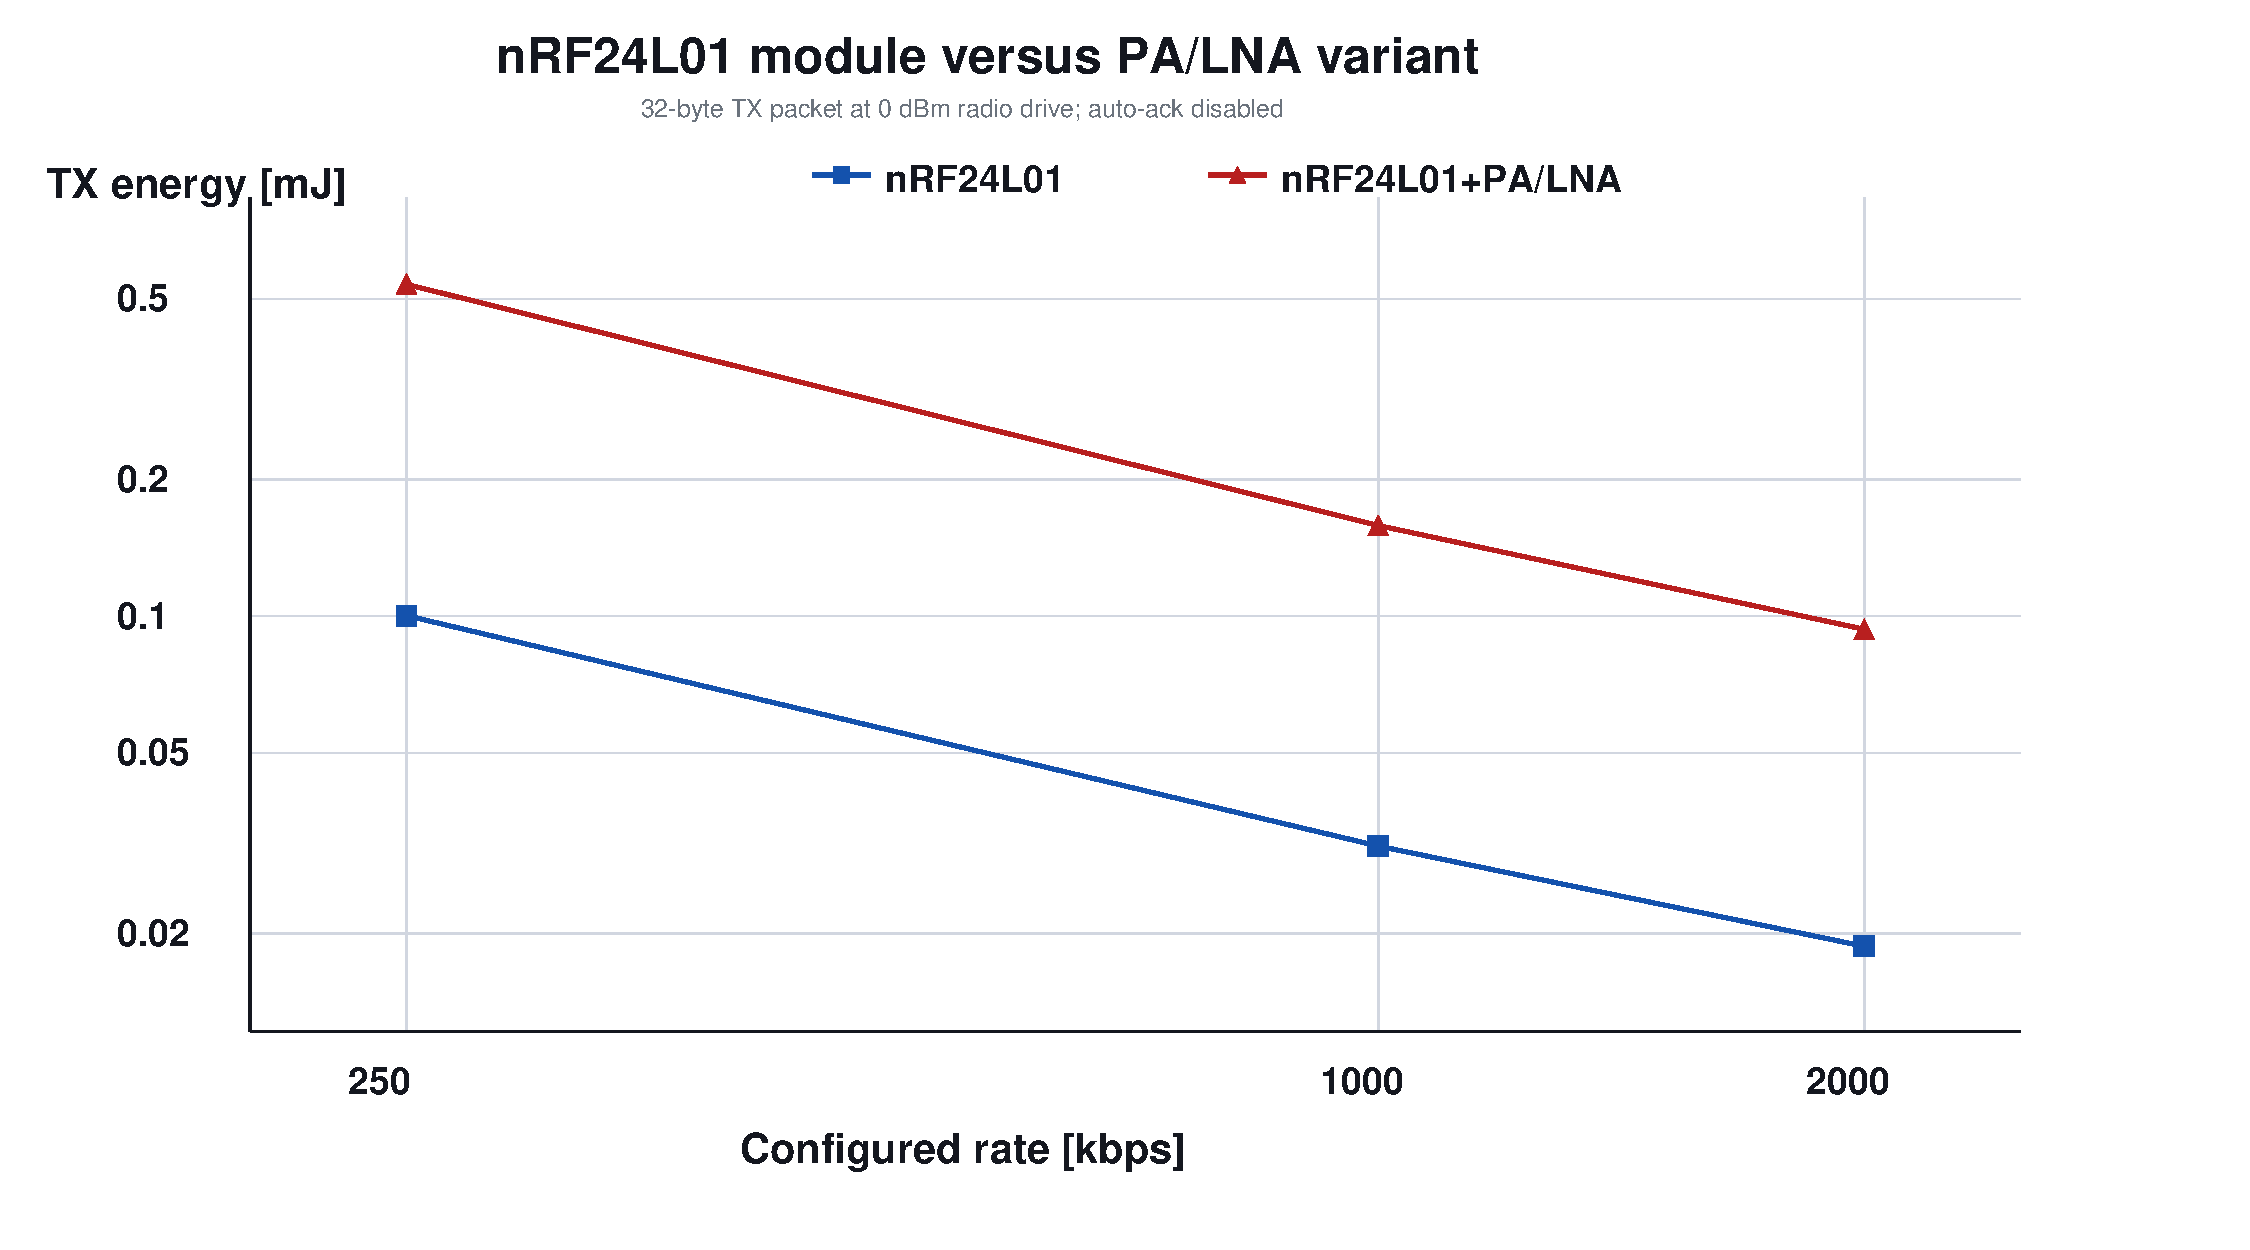
\includegraphics[width=0.93\linewidth]{figures/nrf24_pa_comparison.pdf}
  \caption{nRF24L01 packet TX energy versus rate with and without the module-level PA/LNA. Both use the same 0 dBm radio-drive command.}
  \label{fig:nrf-pa}
\end{figure}

\begin{figure}[htbp]
  \centering
  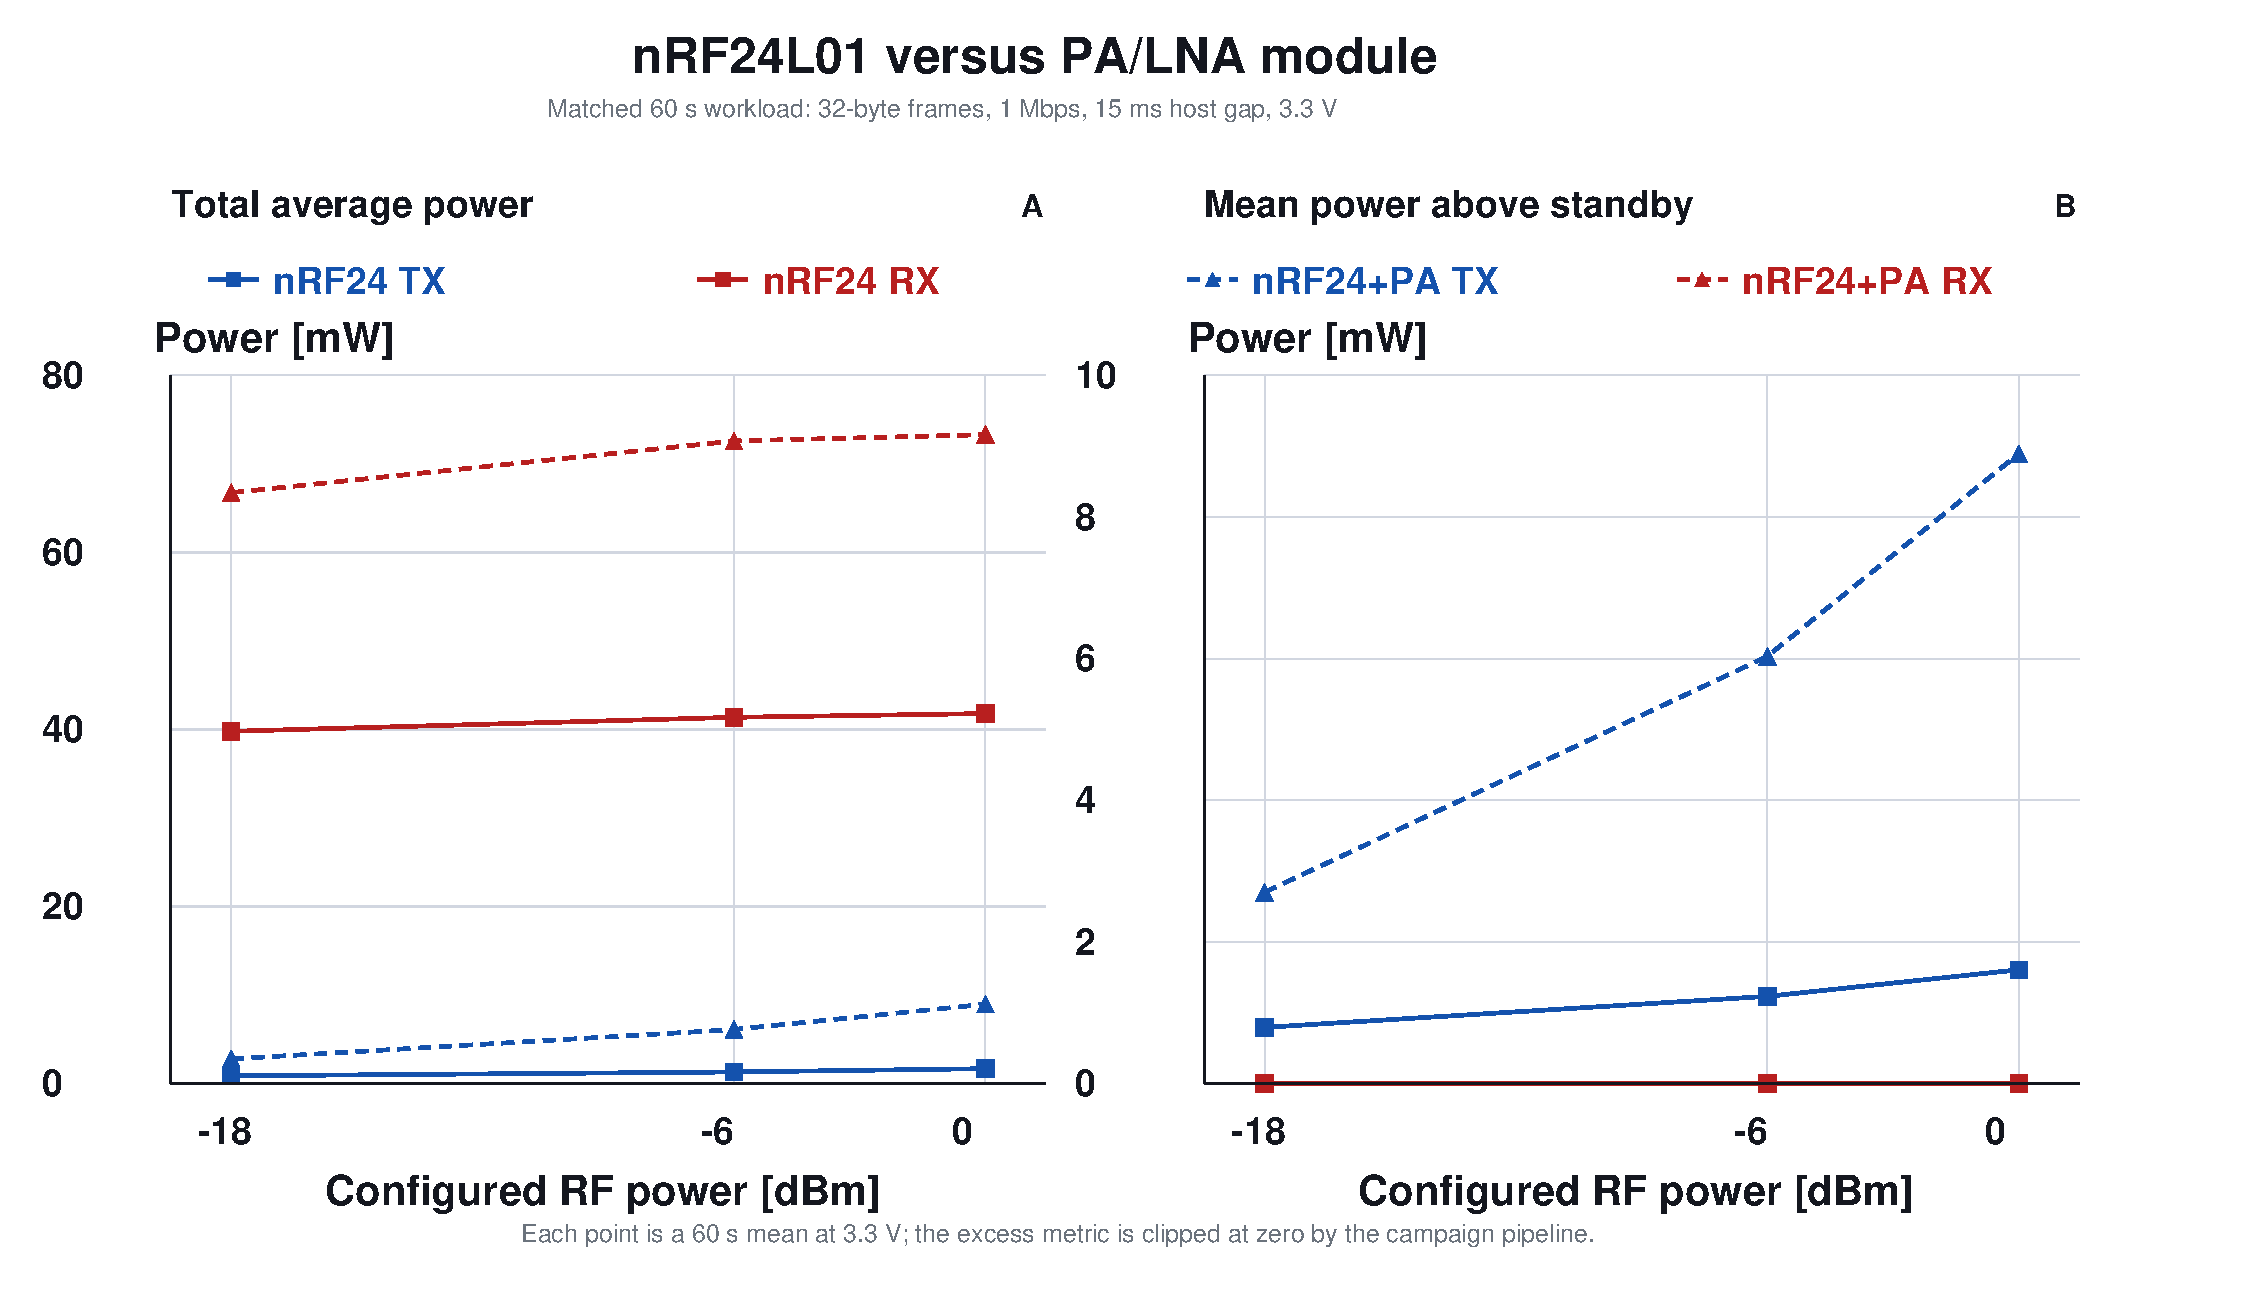
\includegraphics[width=0.96\linewidth]{figures/nrf24_pa_continuous_power_comparison.pdf}
  \caption{Matched nRF24L01 continuous-power comparison at \SI{1}{Mbps}. The PA/LNA module increases both TX and RX module-boundary power across all three configured radio-drive settings.}
  \label{fig:nrf-pa-continuous}
\end{figure}

At \SI{2}{Mbps}, the PA/LNA board uses \SI{0.0935}{mJ} per TX event versus \SI{0.0187}{mJ} for the plain module, almost exactly \num{5.0} times as much. In matched \SI{1}{Mbps} continuous windows, TX power rises from \SI{1.69}{mW} to \SI{8.98}{mW}, and RX power from \SI{41.8}{mW} to \SI{73.3}{mW}. Across the drive sweep, the PA/LNA TX-power multiplier grows from 3.17 at $-18$ dBm to 5.30 at 0 dBm, while total RX power remains 1.68--1.75 times that of the plain module. The zero RX excess values in Figure~\ref{fig:nrf-pa-continuous} are baseline-clamped, not zero total consumption. The PA/LNA variant also delivered fewer frames in this bench setup. This does not imply that an external PA is intrinsically undesirable: its purpose is link budget. It shows that its energy cost must be justified with range or reliability measurements at the intended distance and supply quality.

\begin{figure}[htbp]
  \centering
  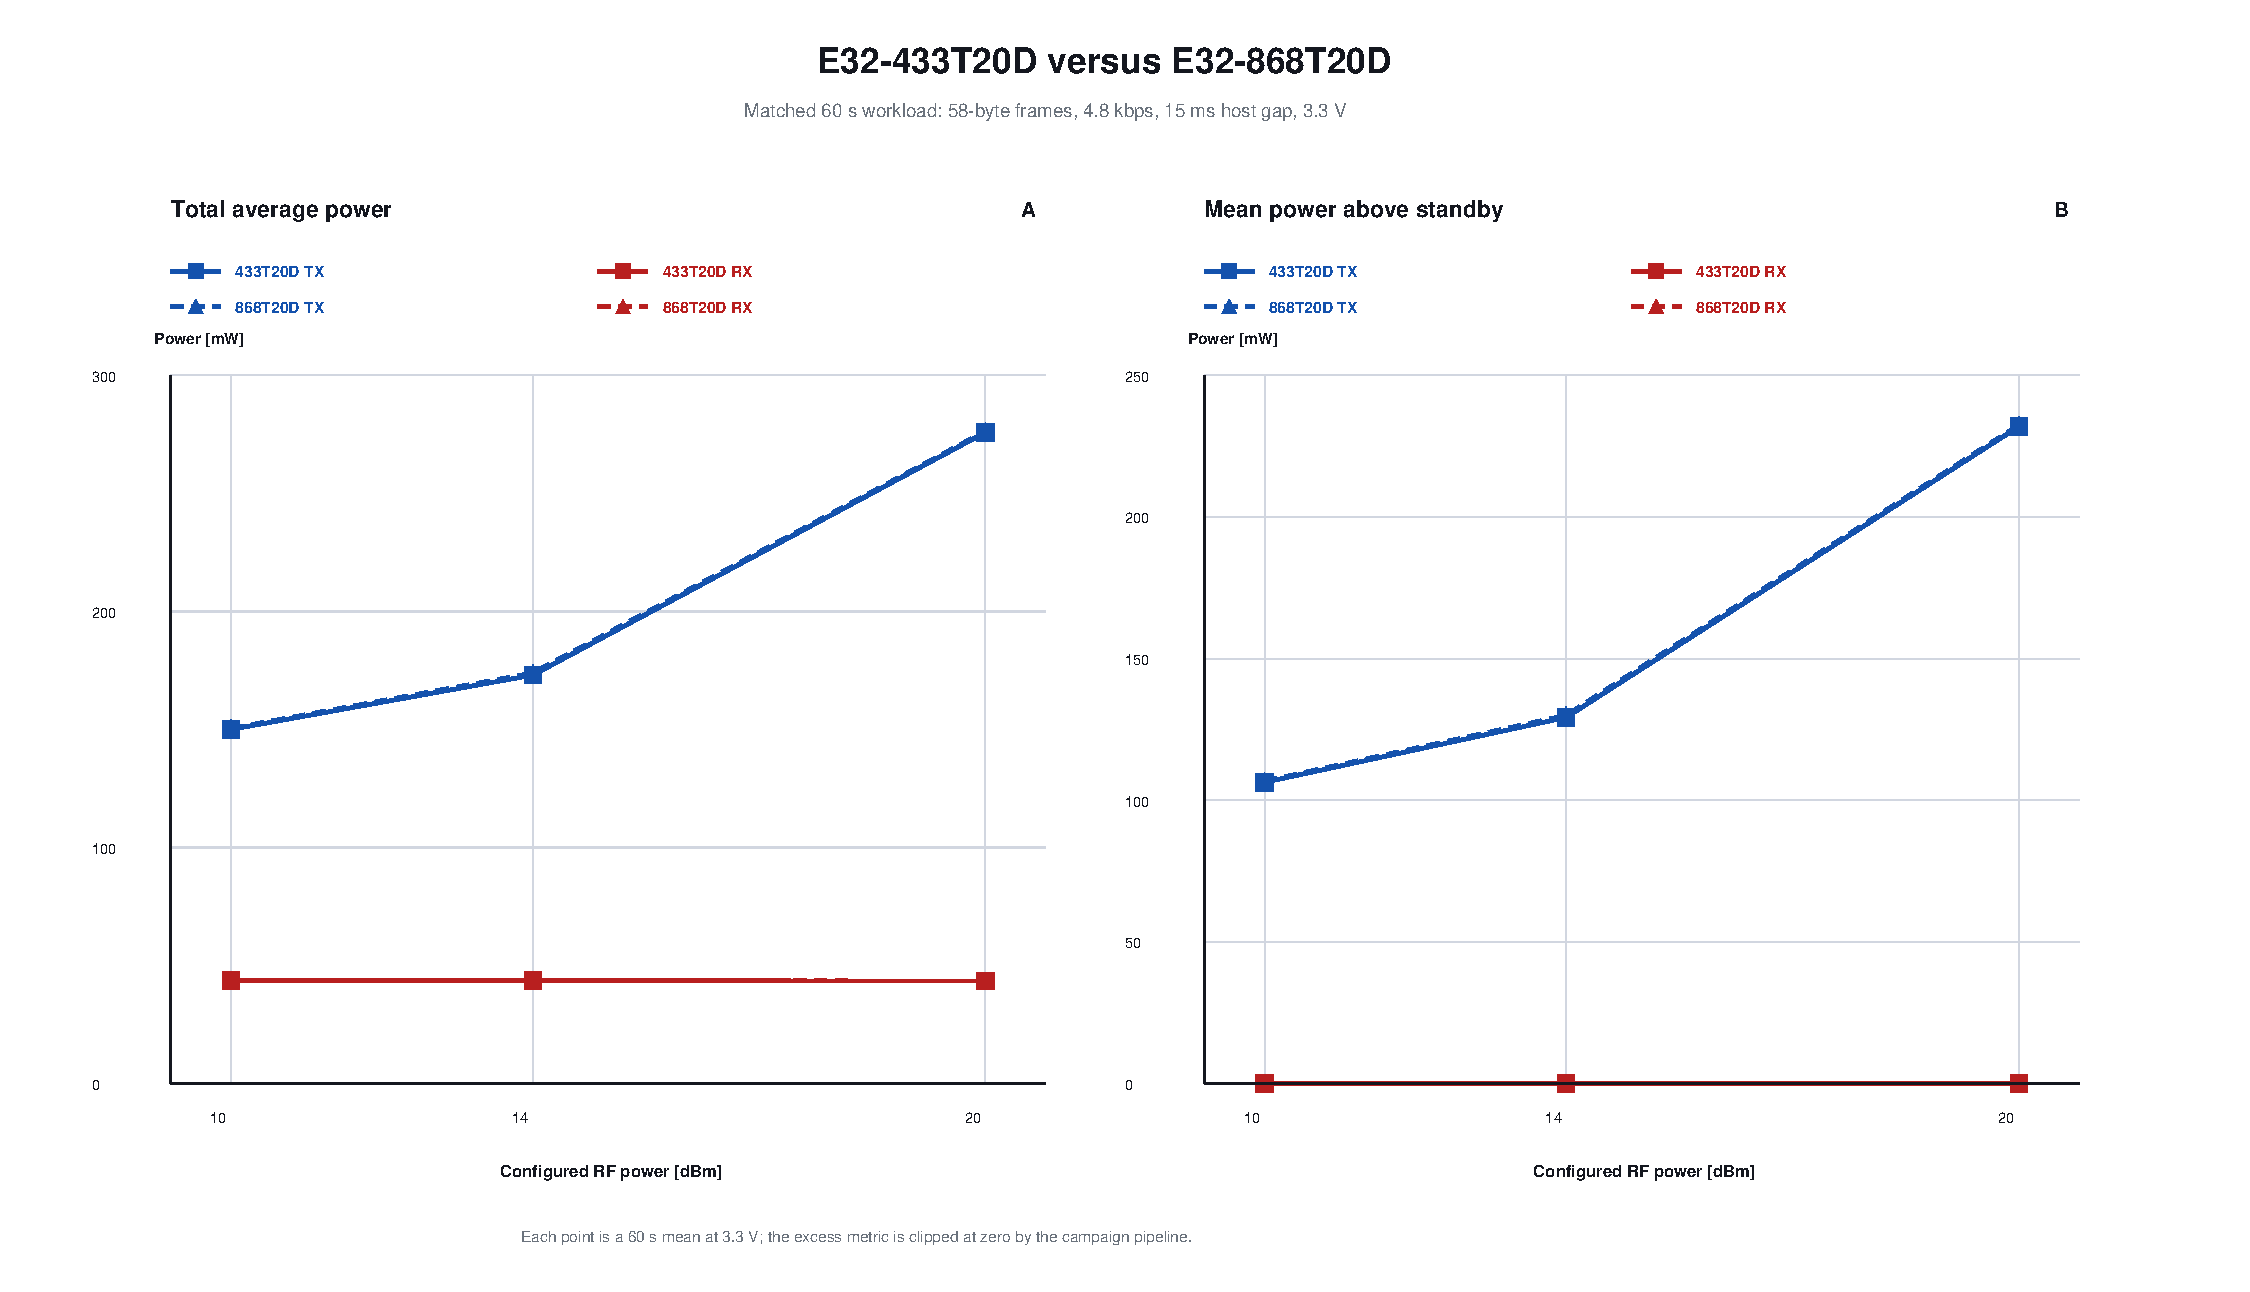
\includegraphics[width=0.96\linewidth]{figures/e32_band_continuous_power_comparison.pdf}
  \caption{Matched continuous-power comparison of the E32-433T20D and E32-868T20D. The nearly coincident curves show that these two measured modules behave alike under the common \SI{4.8}{kbps} workload.}
  \label{fig:e32-band-continuous}
\end{figure}

The E32 20-dBm pair is the closest hardware match in the continuous campaign. At +20 dBm, E32-433T20D and E32-868T20D average \SI{275.86}{mW} and \SI{276.37}{mW} TX, while RX is \SI{43.441}{mW} and \SI{43.438}{mW}. Across all three power settings, the maximum TX difference is \SI{0.52}{\percent} and the maximum RX difference is \SI{0.11}{\percent}. The RX standby-subtracted curve is clipped to zero by the campaign pipeline because the active-window mean falls below its separate standby estimate; it must not be interpreted as a zero-power receiver. Total RX power is the valid comparison in this case.

\clearpage
\section{Discussion}

\subsection{Design implications}

For short, frequent, nearby transfers, the measured high-rate nRF24L01 and E79 GFSK profiles minimize packet airtime and absolute event energy at the common 32-byte workload. Payload curves show why application batching matters: a larger message costs more total energy but generally less energy per application byte. E79 is especially flexible because one firmware image can trade GFSK speed for SLR robustness, OOK behavior, or IEEE 802.15.4g framing. For long-range low-duty-cycle sensing, the SX1262 implementation provides a strong measured RX-power advantage over SX1276/SX1278 boards while retaining a high output-power setting. High-power E32 UART modules simplify integration and provide substantial nominal output power, but their energy and buffering behavior make them a poor fit for frequent battery-powered traffic unless the link budget requires them.

The matched-pair curves sharpen two different lessons. E32-433T20D and E32-868T20D remain nearly indistinguishable under the tested workload, whereas the two CC1101 modules diverge strongly on TX despite sharing the same radio IC. A chipset name is therefore insufficient to predict module energy, but neither should every band or board revision be assumed to matter equally. Antenna size, propagation, legal channels, and interference remain consequential outside these energy traces.

\subsection{What this study does not measure}

No RF power meter, calibrated attenuator chain, conducted sensitivity setup, spectrum analyzer, or controlled-distance range course is part of this dataset. Configured dBm is a command or front-stage setting, not verified conducted output or EIRP. The study cannot compute joules per successfully delivered bit at equal range or equal fade margin. It also cannot rank coexistence, adjacent-channel rejection, antenna efficiency, spectral compliance, or immunity to real interference.

Temperature, unit-to-unit variation, battery internal resistance, and supply voltage were not swept. Five packet repetitions characterize repeatability at each point but are not a production tolerance study. Some continuous campaigns intentionally retain no-RX scenarios and receiver re-arm limitations. Instrument accuracy, automatic range switching, event segmentation, modeled capture windows, and serial telemetry are additional uncertainty sources.

Finally, total event energy is workload-dependent. It is the appropriate quantity for battery budgeting with the tested firmware, but a silicon-only comparison should instead use conducted RF instrumentation and carefully separated idle, synthesizer, ramp, TX, RX, and host-processing intervals.

\section{Reproducibility}

The complete derivation is generated with only the Python standard library and the repository's dependency-free PDF/PNG canvas:
\begin{verbatim}
python power_profiler/study/generate_study.py
pdflatex -interaction=nonstopmode radio_module_energy_study.tex
pdflatex -interaction=nonstopmode radio_module_energy_study.tex
\end{verbatim}
Run the LaTeX commands from \code{power\_profiler/study}. The generated \code{data/module\_summary.csv} records the common 32-byte row selection, delivery scope, packet counts, selected modes, and derived metrics. The companion \code{data/payload\_energy\_summary.csv} records every TX/RX payload point used by Tables~\ref{tab:packet-tx-matrix} and~\ref{tab:packet-rx-matrix}, including the secondary per-bit normalization. The controlled CC1101 points and the E32, nRF24L01, and RA-02 continuous sweeps are exported separately as \code{data/cc1101\_controlled\_summary.csv} and \code{data/matched\_continuous\_power\_summary.csv}. Individual campaign validation notes and audit JSON files remain authoritative for accepted recoveries and known anomalies.

\section{Conclusion}

The measurements show that payload size, radio choice, PHY rate, module implementation, and output stage each materially affect energy. Across the common 32-byte points, fast GFSK devices minimize measured event energy, while high-output transparent LoRa modules incur the greatest cost. The payload matrices show the absolute energy of realistic messages and expose campaign-specific frame and fragmentation boundaries. The E79 within-device study demonstrates a \ESeventyNineImprovement-fold 32-byte packet-energy swing from SLR2K5 to GFSK200 without changing hardware. The SX1278 and nRF24L01 sub-studies show that board-level components can shift energy even when the nominal radio settings are held constant.

The practical conclusion is not that one module wins every application. It is that module selection should be made with a workload-specific point containing payload, rate, output power, receive duty, required link margin, and delivered traffic behavior. This dataset supplies the energy half of that decision and identifies the next necessary experiment: conducted or distance-controlled link-budget and packet-error-rate testing under equal reliability targets.

\begin{thebibliography}{9}

\bibitem{nordic_ppk2}
Nordic Semiconductor, ``Power Profiler Kit II User Guide,'' 2026. [Online]. Available: \url{https://docs.nordicsemi.com/r/bundle/ug_ppk2/page/ug/ppk/ppk_user_guide_intro.html}

\bibitem{ti_cc1101}
Texas Instruments, ``CC1101 Low-Power Sub-1 GHz RF Transceiver Datasheet,'' Rev. I. [Online]. Available: \url{https://www.ti.com/lit/ds/symlink/cc1101.pdf}

\bibitem{ti_cc1352p}
Texas Instruments, ``CC1352P SimpleLink High-Performance Multi-Band Wireless MCU with Integrated Power Amplifier Datasheet,'' Rev. F, 2021. [Online]. Available: \url{https://www.ti.com/lit/ds/symlink/cc1352p.pdf}

\bibitem{nordic_nrf24}
Nordic Semiconductor, ``nRF24L01+ Product Specification,'' v1.0, 2008. [Online]. Available: \url{https://docs-be.nordicsemi.com/bundle/nRF24L01P_PS_v1.0/raw/resource/enus/nRF24L01P_PS_v1.0.pdf}

\bibitem{semtech_sx1276}
Semtech, ``SX1276/77/78/79 LoRa Transceiver Datasheet and Product Information,'' 2020. [Online]. Available: \url{https://www.semtech.com/products/wireless-rf/lora-connect/sx1276}

\bibitem{semtech_sx1262}
Semtech, ``SX1261/SX1262 LoRa Transceiver Datasheet and Product Information,'' 2025. [Online]. Available: \url{https://www.semtech.com/products/wireless-rf/lora-connect/sx1262}

\bibitem{semtech_sx1280}
Semtech, ``SX1280 2.4 GHz LoRa Transceiver Datasheet and Product Information,'' 2023. [Online]. Available: \url{https://www.semtech.com/products/wireless-rf/lora-connect/sx1280}

\bibitem{ebyte_e79}
Chengdu Ebyte, ``E79-400DM2005S Product Specification.'' [Online]. Available: \url{https://www.cdebyte.com/products/E79-400DM2005S/1}

\bibitem{aithinker_ra}
Ai-Thinker, ``Ra-01SH Specification,'' v1.1, 2020. [Online]. Available: \url{https://docs.ai-thinker.com/_media/ra-01sh_specification.pdf}

\end{thebibliography}

\end{document}
